\documentclass[twoside]{book}

% Packages required by doxygen
\usepackage{fixltx2e}
\usepackage{calc}
\usepackage{doxygen}
\usepackage[export]{adjustbox} % also loads graphicx
\usepackage{graphicx}
\usepackage[utf8]{inputenc}
\usepackage{makeidx}
\usepackage{multicol}
\usepackage{multirow}
\PassOptionsToPackage{warn}{textcomp}
\usepackage{textcomp}
\usepackage[nointegrals]{wasysym}
\usepackage[table]{xcolor}

% Font selection
\usepackage[T1]{fontenc}
\usepackage[scaled=.90]{helvet}
\usepackage{courier}
\usepackage{amssymb}
\usepackage{sectsty}
\renewcommand{\familydefault}{\sfdefault}
\allsectionsfont{%
  \fontseries{bc}\selectfont%
  \color{darkgray}%
}
\renewcommand{\DoxyLabelFont}{%
  \fontseries{bc}\selectfont%
  \color{darkgray}%
}
\newcommand{\+}{\discretionary{\mbox{\scriptsize$\hookleftarrow$}}{}{}}

% Page & text layout
\usepackage{geometry}
\geometry{%
  a4paper,%
  top=2.5cm,%
  bottom=2.5cm,%
  left=2.5cm,%
  right=2.5cm%
}
\tolerance=750
\hfuzz=15pt
\hbadness=750
\setlength{\emergencystretch}{15pt}
\setlength{\parindent}{0cm}
\setlength{\parskip}{3ex plus 2ex minus 2ex}
\makeatletter
\renewcommand{\paragraph}{%
  \@startsection{paragraph}{4}{0ex}{-1.0ex}{1.0ex}{%
    \normalfont\normalsize\bfseries\SS@parafont%
  }%
}
\renewcommand{\subparagraph}{%
  \@startsection{subparagraph}{5}{0ex}{-1.0ex}{1.0ex}{%
    \normalfont\normalsize\bfseries\SS@subparafont%
  }%
}
\makeatother

% Headers & footers
\usepackage{fancyhdr}
\pagestyle{fancyplain}
\fancyhead[LE]{\fancyplain{}{\bfseries\thepage}}
\fancyhead[CE]{\fancyplain{}{}}
\fancyhead[RE]{\fancyplain{}{\bfseries\leftmark}}
\fancyhead[LO]{\fancyplain{}{\bfseries\rightmark}}
\fancyhead[CO]{\fancyplain{}{}}
\fancyhead[RO]{\fancyplain{}{\bfseries\thepage}}
\fancyfoot[LE]{\fancyplain{}{}}
\fancyfoot[CE]{\fancyplain{}{}}
\fancyfoot[RE]{\fancyplain{}{\bfseries\scriptsize Generated by Doxygen }}
\fancyfoot[LO]{\fancyplain{}{\bfseries\scriptsize Generated by Doxygen }}
\fancyfoot[CO]{\fancyplain{}{}}
\fancyfoot[RO]{\fancyplain{}{}}
\renewcommand{\footrulewidth}{0.4pt}
\renewcommand{\chaptermark}[1]{%
  \markboth{#1}{}%
}
\renewcommand{\sectionmark}[1]{%
  \markright{\thesection\ #1}%
}

% Indices & bibliography
\usepackage{natbib}
\usepackage[titles]{tocloft}
\setcounter{tocdepth}{3}
\setcounter{secnumdepth}{5}
\makeindex

% Hyperlinks (required, but should be loaded last)
\usepackage{ifpdf}
\ifpdf
  \usepackage[pdftex,pagebackref=true]{hyperref}
\else
  \usepackage[ps2pdf,pagebackref=true]{hyperref}
\fi
\hypersetup{%
  colorlinks=true,%
  linkcolor=blue,%
  citecolor=blue,%
  unicode%
}

% Custom commands
\newcommand{\clearemptydoublepage}{%
  \newpage{\pagestyle{empty}\cleardoublepage}%
}

\usepackage{caption}
\captionsetup{labelsep=space,justification=centering,font={bf},singlelinecheck=off,skip=4pt,position=top}

%===== C O N T E N T S =====

\begin{document}

% Titlepage & ToC
\hypersetup{pageanchor=false,
             bookmarksnumbered=true,
             pdfencoding=unicode
            }
\pagenumbering{roman}
\begin{titlepage}
\vspace*{7cm}
\begin{center}%
{\Large R\+A\+P\+I\+DO }\\
\vspace*{1cm}
{\large Generated by Doxygen 1.8.11}\\
\end{center}
\end{titlepage}
\clearemptydoublepage
\tableofcontents
\clearemptydoublepage
\pagenumbering{arabic}
\hypersetup{pageanchor=true}

%--- Begin generated contents ---
\chapter{R\+A\+P\+I\+DO}
\label{index}\hypertarget{index}{}\label{index_md__Users_jguiang_Projects_rapido_README}%
\Hypertarget{index_md__Users_jguiang_Projects_rapido_README}%
{\itshape Repeatable Analysis Programming for Interpretability, Durability, and Organization}

\href{https://opensource.org/licenses/MIT}{\texttt{ }} \href{https://jkguiang.github.io/rapido/html/index.html}{\texttt{ }} \href{https://www.codefactor.io/repository/github/jkguiang/rapido/overview/master}{\texttt{ }}

RAPIDO is a C++ framework designed to make writing HEP analyses more ergonomic and readable. It wraps some basic functionality of \href{https://root.cern/}{\texttt{ ROOT}}. The idea is that an analysis, in general, consists of a few objects\+: a TTree (to hold some skimmed N-\/\+Tuple and/or a set of histograms), a cutflow (a collection of boolean logic for filtering events), and a looper (some way to run over multiple files). RAPIDO is designed to handle all three of these tasks such that every analysis that uses it is structured in the same way. In addition, the {\itshape way} in which it is structured lends itself to the common workflow of a HEPEx-\/er.\hypertarget{index_autotoc_md1}{}\doxysection{RAPIDO Tools}\label{index_autotoc_md1}

\begin{DoxyEnumerate}
\item \mbox{\hyperlink{classArbol}{Arbol}}\+: TTree wrapper that reduces the hassle of setting up and using TTrees
\item \mbox{\hyperlink{classCutflow}{Cutflow}}\+: Binary search tree with lambda nodes and other bells and whistles
\begin{DoxyItemize}
\item \mbox{\hyperlink{classHistflow}{Histflow}}\+: An extension of the \mbox{\hyperlink{classCutflow}{Cutflow}} object that handles histogramming at any given step of the cutflow
\end{DoxyItemize}
\item \mbox{\hyperlink{classLooper}{Looper}}\+: Basic looper for a TChain of TFiles that uses any selector
\end{DoxyEnumerate}\hypertarget{index_autotoc_md2}{}\doxysection{Set Up Instructions}\label{index_autotoc_md2}

\begin{DoxyEnumerate}
\item Clone this repository
\item {\ttfamily cd} into the cloned repository and run {\ttfamily make -\/j5}
\item Write your script (e.\+g. {\ttfamily main.\+cc}) and {\ttfamily \#include} whatever you need
\item Compile and run using your favorite {\ttfamily Makefile}\+: 
\begin{DoxyCode}{0}
\DoxyCodeLine{\$ make}
\DoxyCodeLine{\$ export LD\_LIBRARY\_PATH=\$LD\_LIBRARY\_PATH:\$PWD/rapido/src}
\DoxyCodeLine{\$ export ROOT\_INCLUDE\_PATH=\$ROOT\_INCLUDE\_PATH:\$PWD/rapido/src}
\DoxyCodeLine{\$ ./main}

\end{DoxyCode}

\end{DoxyEnumerate}\hypertarget{index_autotoc_md3}{}\doxysection{Examples}\label{index_autotoc_md3}

\begin{DoxyEnumerate}
\item Minimal \mbox{\hyperlink{classCutflow}{Cutflow}} example 
\begin{DoxyCode}{0}
\DoxyCodeLine{\textcolor{preprocessor}{\#include "{}cutflow.h"{}}}
\DoxyCodeLine{\textcolor{preprocessor}{\#include <stdlib.h>}}
\DoxyCodeLine{}
\DoxyCodeLine{\textcolor{keyword}{using} namepsace std;}
\DoxyCodeLine{}
\DoxyCodeLine{\textcolor{keywordtype}{int} main()}
\DoxyCodeLine{\{}
\DoxyCodeLine{    \mbox{\hyperlink{classCutflow}{Cutflow}} dummy\_cutflow = \mbox{\hyperlink{classCutflow}{Cutflow}}();}
\DoxyCodeLine{}
\DoxyCodeLine{    \mbox{\hyperlink{classCut}{Cut}}* dummy\_root = \textcolor{keyword}{new} \mbox{\hyperlink{classCut}{Cut}}(\textcolor{stringliteral}{"{}root"{}}, []() \{ \textcolor{keywordflow}{return} bool(rand() \% 2); \});}
\DoxyCodeLine{    dummy\_cutflow.\mbox{\hyperlink{classCutflow_ad27d37141c3748779a5d81fad919ecbb}{setRoot}}(dummy\_root);}
\DoxyCodeLine{}
\DoxyCodeLine{    \mbox{\hyperlink{classCut}{Cut}}* node0 = \textcolor{keyword}{new} \mbox{\hyperlink{classCut}{Cut}}(\textcolor{stringliteral}{"{}node0"{}}, []() \{ \textcolor{keywordflow}{return} bool(rand() \% 2); \});}
\DoxyCodeLine{    dummy\_cutflow.\mbox{\hyperlink{classCutflow_a8da46f1053a6b97991489ee0920c29a1}{insert}}(\textcolor{stringliteral}{"{}root"{}}, node0, Left);}
\DoxyCodeLine{}
\DoxyCodeLine{    \mbox{\hyperlink{classCut}{Cut}}* node1 = \textcolor{keyword}{new} \mbox{\hyperlink{classCut}{Cut}}(\textcolor{stringliteral}{"{}node1"{}}, []() \{ \textcolor{keywordflow}{return} bool(rand() \% 2); \});}
\DoxyCodeLine{    dummy\_cutflow.\mbox{\hyperlink{classCutflow_a8da46f1053a6b97991489ee0920c29a1}{insert}}(\textcolor{stringliteral}{"{}root"{}}, node1, Right);}
\DoxyCodeLine{}
\DoxyCodeLine{    \mbox{\hyperlink{classCut}{Cut}}* node2 = \textcolor{keyword}{new} \mbox{\hyperlink{classCut}{Cut}}(\textcolor{stringliteral}{"{}node2"{}}, []() \{ \textcolor{keywordflow}{return} bool(rand() \% 2); \});}
\DoxyCodeLine{    dummy\_cutflow.\mbox{\hyperlink{classCutflow_a8da46f1053a6b97991489ee0920c29a1}{insert}}(\textcolor{stringliteral}{"{}node1"{}}, node2, Right);}
\DoxyCodeLine{}
\DoxyCodeLine{    \mbox{\hyperlink{classCut}{Cut}}* node3 = \textcolor{keyword}{new} \mbox{\hyperlink{classCut}{Cut}}(\textcolor{stringliteral}{"{}node3"{}}, []() \{ \textcolor{keywordflow}{return} bool(rand() \% 2); \});}
\DoxyCodeLine{    dummy\_cutflow.\mbox{\hyperlink{classCutflow_a8da46f1053a6b97991489ee0920c29a1}{insert}}(\textcolor{stringliteral}{"{}node1"{}}, node3, Left);}
\DoxyCodeLine{}
\DoxyCodeLine{    \mbox{\hyperlink{classCut}{Cut}}* node4 = \textcolor{keyword}{new} \mbox{\hyperlink{classCut}{Cut}}(\textcolor{stringliteral}{"{}node4"{}}, []() \{ \textcolor{keywordflow}{return} bool(rand() \% 2); \});}
\DoxyCodeLine{    dummy\_cutflow.\mbox{\hyperlink{classCutflow_a8da46f1053a6b97991489ee0920c29a1}{insert}}(\textcolor{stringliteral}{"{}node2"{}}, node4, Right);}
\DoxyCodeLine{}
\DoxyCodeLine{    \textcolor{keywordflow}{for} (\textcolor{keywordtype}{int} i = 0; i < 5; i++)}
\DoxyCodeLine{    \{}
\DoxyCodeLine{        \mbox{\hyperlink{classCut}{Cut}}* terminal\_node = dummy\_cutflow.\mbox{\hyperlink{classCutflow_a563da4fc41aa5c611dd0ce37ce966f2c}{run}}();}
\DoxyCodeLine{        cout << \textcolor{stringliteral}{"{}terminated at "{}} << terminal\_node-\/>\mbox{\hyperlink{classCut_accf700d2d00746b97a265d4aea3f55c2}{name}} << endl;}
\DoxyCodeLine{    \}}
\DoxyCodeLine{    dummy\_cutflow.\mbox{\hyperlink{classCutflow_a0cb4c8bd6d15ace1f85fe0cfb8d9d828}{print}}();}
\DoxyCodeLine{}
\DoxyCodeLine{    \textcolor{keywordflow}{return} 0;}
\DoxyCodeLine{\}}

\end{DoxyCode}

\item A simple Arbol+\+Looper example (using {\ttfamily ROOT\+::\+Make\+Selector} to read an arbitrary ROOT file) 
\begin{DoxyCode}{0}
\DoxyCodeLine{\$ root \# only known to work for ROOT v6.22 and greater}
\DoxyCodeLine{root[0] TFile* f = new TFile("{}/path/to/myfile.root"{})}
\DoxyCodeLine{root[1] TreeName-\/>MakeSelector("{}MySelector"{})}
\DoxyCodeLine{(int) 0}
\DoxyCodeLine{root [2] .q}
\DoxyCodeLine{\$ mv MySelector.C MySelector.cc}
\DoxyCodeLine{\$ rootcint myselectordict.cc -\/c MySelector.h}
\DoxyCodeLine{\$ mv myselectordict* rapdio/}
\DoxyCodeLine{\$ mv MySelector* rapido/}
\DoxyCodeLine{\$ cd rapido/}
\DoxyCodeLine{\$ make clean}
\DoxyCodeLine{\$ make -\/j5}

\end{DoxyCode}
 
\begin{DoxyCode}{0}
\DoxyCodeLine{\textcolor{comment}{// Selector}}
\DoxyCodeLine{\textcolor{preprocessor}{\#include "{}MySelector.h"{}}}
\DoxyCodeLine{\textcolor{comment}{// RAPIDO}}
\DoxyCodeLine{\textcolor{preprocessor}{\#include "{}arbol.h"{}}}
\DoxyCodeLine{\textcolor{preprocessor}{\#include "{}looper.h"{}}}
\DoxyCodeLine{}
\DoxyCodeLine{\textcolor{keywordtype}{int} main()}
\DoxyCodeLine{\{}
\DoxyCodeLine{    \textcolor{comment}{// Initialize Arbol}}
\DoxyCodeLine{    TFile* output\_tfile = \textcolor{keyword}{new} Tfile(\textcolor{stringliteral}{"{}output.root"{}}, \textcolor{stringliteral}{"{}RECREATE"{}});}
\DoxyCodeLine{    \mbox{\hyperlink{classArbol}{Arbol}} arbol = \mbox{\hyperlink{classArbol}{Arbol}}(output\_tfile);}
\DoxyCodeLine{}
\DoxyCodeLine{    \textcolor{comment}{// Initialize branches}}
\DoxyCodeLine{    arbol.\mbox{\hyperlink{classArbol_a552622885ffce15f1b1369fe44e729bb}{newBranch}}<\textcolor{keywordtype}{int}>(\textcolor{stringliteral}{"{}event"{}});}
\DoxyCodeLine{    arbol.\mbox{\hyperlink{classArbol_a552622885ffce15f1b1369fe44e729bb}{newBranch}}<\textcolor{keywordtype}{float}>(\textcolor{stringliteral}{"{}met"{}});}
\DoxyCodeLine{    arbol.\mbox{\hyperlink{classArbol_a552622885ffce15f1b1369fe44e729bb}{newBranch}}<\textcolor{keywordtype}{float}>(\textcolor{stringliteral}{"{}ht"{}});}
\DoxyCodeLine{    arbol.\mbox{\hyperlink{classArbol_a552622885ffce15f1b1369fe44e729bb}{newBranch}}<\textcolor{keywordtype}{int}>(\textcolor{stringliteral}{"{}n\_jets"{}});}
\DoxyCodeLine{    arbol.\mbox{\hyperlink{classArbol_a57b6cf7cca6cbb3b75bb0e0333dbe3c8}{newVecBranch}}<\textcolor{keywordtype}{float}>(\textcolor{stringliteral}{"{}good\_jet\_pt"{}}); \textcolor{comment}{// newVecBranch<float> <-\/-\/> newBranch<std::vector<float>>}}
\DoxyCodeLine{}
\DoxyCodeLine{    \textcolor{comment}{// Get file}}
\DoxyCodeLine{    TChain* tchain = \textcolor{keyword}{new} TChain(\textcolor{stringliteral}{"{}TreeName"{}}); }
\DoxyCodeLine{    tchain-\/>Add(\textcolor{stringliteral}{"{}/path/to/myfile.root"{}});}
\DoxyCodeLine{}
\DoxyCodeLine{    \textcolor{comment}{// Initialize Looper}}
\DoxyCodeLine{    MySelector selector;}
\DoxyCodeLine{    \mbox{\hyperlink{classLooper}{Looper}} looper = \mbox{\hyperlink{classLooper}{Looper<Nano>}}(\&selector, tchain, \textcolor{stringliteral}{"{}TreeName"{}});}
\DoxyCodeLine{}
\DoxyCodeLine{    \textcolor{comment}{// Run}}
\DoxyCodeLine{    looper.\mbox{\hyperlink{classLooper_abfa564ca48778da1f58c8a6444ddd463}{run}}(}
\DoxyCodeLine{        [\&]()}
\DoxyCodeLine{        \{}
\DoxyCodeLine{            \textcolor{comment}{// -\/-\/> Event-\/level Logic <-\/-\/}}
\DoxyCodeLine{            \textcolor{comment}{// Reset tree}}
\DoxyCodeLine{            arbol.\mbox{\hyperlink{classArbol_a4c2184d378ab21a9627a57098291a7c4}{resetBranches}}(); \textcolor{comment}{// variables like arbol and selector are captured by reference}}
\DoxyCodeLine{            \textcolor{comment}{// Loop over jets}}
\DoxyCodeLine{            \textcolor{keywordtype}{float} ht = 0.;}
\DoxyCodeLine{            \textcolor{keywordflow}{for} (\textcolor{keywordtype}{unsigned} \textcolor{keywordtype}{int} i = 0; i < *selector.nJet; i++) }
\DoxyCodeLine{            \{}
\DoxyCodeLine{                \textcolor{keywordflow}{if} (selector.Jet\_pt[i] > 30)}
\DoxyCodeLine{                \{}
\DoxyCodeLine{                    arbol.appendToVecLeaf<float>(\textcolor{stringliteral}{"{}good\_jet\_pt"{}}, selector.Jet\_pt[i]);}
\DoxyCodeLine{                    ht += selector.Jet\_pt[i];}
\DoxyCodeLine{                \}}
\DoxyCodeLine{            \}}
\DoxyCodeLine{            arbol.\mbox{\hyperlink{classArbol_a7a8d3bec0bf5c00635a0b00fcd63cf01}{setLeaf}}<\textcolor{keywordtype}{int}>(\textcolor{stringliteral}{"{}event"{}}, *selector.event);}
\DoxyCodeLine{            arbol.\mbox{\hyperlink{classArbol_a7a8d3bec0bf5c00635a0b00fcd63cf01}{setLeaf}}<\textcolor{keywordtype}{float}>(\textcolor{stringliteral}{"{}ht"{}}, ht);}
\DoxyCodeLine{            arbol.\mbox{\hyperlink{classArbol_a7a8d3bec0bf5c00635a0b00fcd63cf01}{setLeaf}}<\textcolor{keywordtype}{float}>(\textcolor{stringliteral}{"{}met"{}}, *selector.MET\_pt);}
\DoxyCodeLine{            arbol.\mbox{\hyperlink{classArbol_a7a8d3bec0bf5c00635a0b00fcd63cf01}{setLeaf}}<\textcolor{keywordtype}{int}>(\textcolor{stringliteral}{"{}n\_jets"{}}, arbol.\mbox{\hyperlink{classArbol_aefdf6dfa74ceed51b2cb99f45bfebf56}{getVecLeaf}}<\textcolor{keywordtype}{float}>(\textcolor{stringliteral}{"{}goot\_jet\_pt"{}}).size());}
\DoxyCodeLine{            arbol.\mbox{\hyperlink{classArbol_a1d029dd97a0451281c774b578d93bcda}{fillTTree}}();}
\DoxyCodeLine{            \textcolor{keywordflow}{return};}
\DoxyCodeLine{        \}}
\DoxyCodeLine{    );}
\DoxyCodeLine{    \textcolor{comment}{// Write results to a ROOT file}}
\DoxyCodeLine{    arbol.\mbox{\hyperlink{classArbol_ade7d835bbe383a70006e86785ae5672c}{writeTFile}}();}
\DoxyCodeLine{    \textcolor{keywordflow}{return} 0;}
\DoxyCodeLine{\}}

\end{DoxyCode}

\item Arbol+\+Cutflow+\+Looper+\+HEPCLI example (now using \href{https://github.com/cmstas/NanoTools/tree/master/NanoCORE}{\texttt{ Nano\+CORE}} to read Nano\+AOD) 
\begin{DoxyCode}{0}
\DoxyCodeLine{\textcolor{comment}{// ROOT}}
\DoxyCodeLine{\textcolor{preprocessor}{\#include "{}TH1F.h"{}}}
\DoxyCodeLine{\textcolor{comment}{// NanoCORE}}
\DoxyCodeLine{\textcolor{preprocessor}{\#include "{}Nano.h"{}}}
\DoxyCodeLine{\textcolor{preprocessor}{\#include "{}tqdm.h"{}} \textcolor{comment}{// progress bar}}
\DoxyCodeLine{\textcolor{preprocessor}{\#include "{}SSSelections.h"{}}}
\DoxyCodeLine{\textcolor{preprocessor}{\#include "{}ElectronSelections.h"{}}}
\DoxyCodeLine{\textcolor{preprocessor}{\#include "{}MuonSelections.h"{}}}
\DoxyCodeLine{\textcolor{comment}{// RAPIDO}}
\DoxyCodeLine{\textcolor{preprocessor}{\#include "{}arbol.h"{}}}
\DoxyCodeLine{\textcolor{preprocessor}{\#include "{}cutflow.h"{}}}
\DoxyCodeLine{\textcolor{preprocessor}{\#include "{}looper.h"{}}}
\DoxyCodeLine{}
\DoxyCodeLine{\textcolor{keyword}{using namespace }std;}
\DoxyCodeLine{\textcolor{keyword}{using namespace }tas;}
\DoxyCodeLine{}
\DoxyCodeLine{\textcolor{keywordtype}{int} main(\textcolor{keywordtype}{int} argc, \textcolor{keywordtype}{char}** argv) }
\DoxyCodeLine{\{}
\DoxyCodeLine{    \textcolor{comment}{// CLI}}
\DoxyCodeLine{    \mbox{\hyperlink{classHEPCLI}{HEPCLI}} cli = \mbox{\hyperlink{classHEPCLI}{HEPCLI}}(argc, argv);}
\DoxyCodeLine{}
\DoxyCodeLine{    \textcolor{comment}{// Initialize Looper}}
\DoxyCodeLine{    \mbox{\hyperlink{classLooper}{Looper}} looper = \mbox{\hyperlink{classLooper}{Looper<Nano>}}(\&nt, cli.\mbox{\hyperlink{classHEPCLI_a3d4bb4a7c1f1b6d4e008ff76e43bef15}{input\_tchain}});}
\DoxyCodeLine{}
\DoxyCodeLine{    \textcolor{comment}{// Initialize Arbol}}
\DoxyCodeLine{    \mbox{\hyperlink{classArbol}{Arbol}} arbol = \mbox{\hyperlink{classArbol}{Arbol}}(cli.\mbox{\hyperlink{classHEPCLI_ab900d2e3822e20d636564874440d33f0}{output\_tfile}});}
\DoxyCodeLine{    \textcolor{comment}{// Event branches}}
\DoxyCodeLine{    arbol.\mbox{\hyperlink{classArbol_a552622885ffce15f1b1369fe44e729bb}{newBranch}}<\textcolor{keywordtype}{int}>(\textcolor{stringliteral}{"{}event"{}}, -\/999);}
\DoxyCodeLine{    arbol.\mbox{\hyperlink{classArbol_a552622885ffce15f1b1369fe44e729bb}{newBranch}}<\textcolor{keywordtype}{float}>(\textcolor{stringliteral}{"{}met"{}}, -\/999);}
\DoxyCodeLine{    \textcolor{comment}{// Leptons}}
\DoxyCodeLine{    arbol.\mbox{\hyperlink{classArbol_a552622885ffce15f1b1369fe44e729bb}{newBranch}}<\textcolor{keywordtype}{int}>(\textcolor{stringliteral}{"{}leading\_lep\_id"{}}, -\/999);}
\DoxyCodeLine{    arbol.\mbox{\hyperlink{classArbol_a552622885ffce15f1b1369fe44e729bb}{newBranch}}<\textcolor{keywordtype}{float}>(\textcolor{stringliteral}{"{}leading\_lep\_pt"{}}, -\/999);}
\DoxyCodeLine{    arbol.\mbox{\hyperlink{classArbol_a552622885ffce15f1b1369fe44e729bb}{newBranch}}<\textcolor{keywordtype}{float}>(\textcolor{stringliteral}{"{}leading\_lep\_eta"{}}, -\/999);}
\DoxyCodeLine{    arbol.\mbox{\hyperlink{classArbol_a552622885ffce15f1b1369fe44e729bb}{newBranch}}<\textcolor{keywordtype}{float}>(\textcolor{stringliteral}{"{}leading\_lep\_phi"{}}, -\/999);}
\DoxyCodeLine{    arbol.\mbox{\hyperlink{classArbol_a552622885ffce15f1b1369fe44e729bb}{newBranch}}<\textcolor{keywordtype}{int}>(\textcolor{stringliteral}{"{}trailing\_lep\_id"{}}, -\/999);}
\DoxyCodeLine{    arbol.\mbox{\hyperlink{classArbol_a552622885ffce15f1b1369fe44e729bb}{newBranch}}<\textcolor{keywordtype}{float}>(\textcolor{stringliteral}{"{}trailing\_lep\_pt"{}}, -\/999);}
\DoxyCodeLine{    arbol.\mbox{\hyperlink{classArbol_a552622885ffce15f1b1369fe44e729bb}{newBranch}}<\textcolor{keywordtype}{float}>(\textcolor{stringliteral}{"{}trailing\_lep\_eta"{}}, -\/999);}
\DoxyCodeLine{    arbol.\mbox{\hyperlink{classArbol_a552622885ffce15f1b1369fe44e729bb}{newBranch}}<\textcolor{keywordtype}{float}>(\textcolor{stringliteral}{"{}trailing\_lep\_phi"{}}, -\/999);}
\DoxyCodeLine{}
\DoxyCodeLine{    \textcolor{comment}{// Initialize Cutflow}}
\DoxyCodeLine{    \mbox{\hyperlink{classCutflow}{Cutflow}} cutflow = \mbox{\hyperlink{classCutflow}{Cutflow}}();}
\DoxyCodeLine{}
\DoxyCodeLine{    \textcolor{comment}{// Initialize some hists}}
\DoxyCodeLine{    TH1F* ld\_lep\_pt\_hist = \textcolor{keyword}{new} TH1F(\textcolor{stringliteral}{"{}ld\_lep\_pt\_hist"{}}, \textcolor{stringliteral}{"{}ld\_lep\_pt\_hist"{}}, 20, 0, 200);}
\DoxyCodeLine{    TH1F* tr\_lep\_pt\_hist = \textcolor{keyword}{new} TH1F(\textcolor{stringliteral}{"{}tr\_lep\_pt\_hist"{}}, \textcolor{stringliteral}{"{}tr\_lep\_pt\_hist"{}}, 20, 0, 200);}
\DoxyCodeLine{    cutflow.globals.newVar<TH1F>(\textcolor{stringliteral}{"{}ld\_lep\_pt\_hist"{}}, *ld\_lep\_pt\_hist);}
\DoxyCodeLine{    cutflow.globals.newVar<TH1F>(\textcolor{stringliteral}{"{}tr\_lep\_pt\_hist"{}}, *tr\_lep\_pt\_hist);}
\DoxyCodeLine{}
\DoxyCodeLine{    \mbox{\hyperlink{classCut}{Cut}}* root = \textcolor{keyword}{new} \mbox{\hyperlink{classCut}{Cut}}(}
\DoxyCodeLine{        \textcolor{stringliteral}{"{}Bookkeeping"{}},}
\DoxyCodeLine{        [\&]()}
\DoxyCodeLine{        \{}
\DoxyCodeLine{            arbol.\mbox{\hyperlink{classArbol_a7a8d3bec0bf5c00635a0b00fcd63cf01}{setLeaf}}(\textcolor{stringliteral}{"{}event"{}}, nt.event());}
\DoxyCodeLine{            arbol.\mbox{\hyperlink{classArbol_a7a8d3bec0bf5c00635a0b00fcd63cf01}{setLeaf}}(\textcolor{stringliteral}{"{}met"{}}, nt.MET\_pt());}
\DoxyCodeLine{            \textcolor{keywordflow}{return} \textcolor{keyword}{true};}
\DoxyCodeLine{        \},}
\DoxyCodeLine{        [\&]()}
\DoxyCodeLine{        \{}
\DoxyCodeLine{            \textcolor{comment}{// Dummy weight}}
\DoxyCodeLine{            \textcolor{keywordflow}{return} 0.001;}
\DoxyCodeLine{        \}}
\DoxyCodeLine{    );}
\DoxyCodeLine{    cutflow.setRoot(root);}
\DoxyCodeLine{}
\DoxyCodeLine{    \mbox{\hyperlink{classCut}{Cut}}* dilep\_presel = \textcolor{keyword}{new} \mbox{\hyperlink{classCut}{Cut}}(}
\DoxyCodeLine{        \textcolor{stringliteral}{"{}DileptonPreselection"{}},}
\DoxyCodeLine{        [\&]()}
\DoxyCodeLine{        \{}
\DoxyCodeLine{            \textcolor{keywordtype}{int} n\_tight\_leps = 0;}
\DoxyCodeLine{            \textcolor{keywordtype}{int} n\_loose\_not\_tight\_leps = 0;}
\DoxyCodeLine{            Leptons leptons = getLeptons();}
\DoxyCodeLine{            Lepton leading\_lep;}
\DoxyCodeLine{            Lepton trailing\_lep;}
\DoxyCodeLine{            \textcolor{keywordflow}{for} (\textcolor{keyword}{auto}\& lep : leptons)}
\DoxyCodeLine{            \{}
\DoxyCodeLine{                \textcolor{keywordflow}{if} (lep.pt() < 20) \{ \textcolor{keywordflow}{continue}; \}}
\DoxyCodeLine{                \textcolor{keywordflow}{if} (lep.idlevel() == SS::IDtight) }
\DoxyCodeLine{                \{ }
\DoxyCodeLine{                    \textcolor{keywordflow}{if} (lep.pt() > leading\_lep.pt()) }
\DoxyCodeLine{                    \{ }
\DoxyCodeLine{                        trailing\_lep = leading\_lep;}
\DoxyCodeLine{                        leading\_lep = lep; }
\DoxyCodeLine{                    \}}
\DoxyCodeLine{                    \textcolor{keywordflow}{else} \textcolor{keywordflow}{if} (lep.pt() > trailing\_lep.pt()) \{ trailing\_lep = lep; \}}
\DoxyCodeLine{                    n\_tight\_leps++; }
\DoxyCodeLine{                \}}
\DoxyCodeLine{                \textcolor{keywordflow}{if} (lep.idlevel() == SS::IDfakable) \{ n\_loose\_not\_tight\_leps++; \}}
\DoxyCodeLine{            \}}
\DoxyCodeLine{            \textcolor{keywordflow}{if} (n\_tight\_leps == 2 \&\& n\_loose\_not\_tight\_leps == 0) }
\DoxyCodeLine{            \{}
\DoxyCodeLine{                arbol.\mbox{\hyperlink{classArbol_a7a8d3bec0bf5c00635a0b00fcd63cf01}{setLeaf}}<\textcolor{keywordtype}{int}>(\textcolor{stringliteral}{"{}leading\_lep\_id"{}}, leading\_lep.id());}
\DoxyCodeLine{                arbol.\mbox{\hyperlink{classArbol_a7a8d3bec0bf5c00635a0b00fcd63cf01}{setLeaf}}<\textcolor{keywordtype}{float}>(\textcolor{stringliteral}{"{}leading\_lep\_pt"{}}, leading\_lep.pt());}
\DoxyCodeLine{                arbol.\mbox{\hyperlink{classArbol_a7a8d3bec0bf5c00635a0b00fcd63cf01}{setLeaf}}<\textcolor{keywordtype}{float}>(\textcolor{stringliteral}{"{}leading\_lep\_eta"{}}, leading\_lep.eta());}
\DoxyCodeLine{                arbol.\mbox{\hyperlink{classArbol_a7a8d3bec0bf5c00635a0b00fcd63cf01}{setLeaf}}<\textcolor{keywordtype}{float}>(\textcolor{stringliteral}{"{}leading\_lep\_phi"{}}, leading\_lep.phi());}
\DoxyCodeLine{                arbol.\mbox{\hyperlink{classArbol_a7a8d3bec0bf5c00635a0b00fcd63cf01}{setLeaf}}<\textcolor{keywordtype}{int}>(\textcolor{stringliteral}{"{}trailing\_lep\_id"{}}, trailing\_lep.id());}
\DoxyCodeLine{                arbol.\mbox{\hyperlink{classArbol_a7a8d3bec0bf5c00635a0b00fcd63cf01}{setLeaf}}<\textcolor{keywordtype}{float}>(\textcolor{stringliteral}{"{}trailing\_lep\_pt"{}}, trailing\_lep.pt());}
\DoxyCodeLine{                arbol.\mbox{\hyperlink{classArbol_a7a8d3bec0bf5c00635a0b00fcd63cf01}{setLeaf}}<\textcolor{keywordtype}{float}>(\textcolor{stringliteral}{"{}trailing\_lep\_eta"{}}, trailing\_lep.eta());}
\DoxyCodeLine{                arbol.\mbox{\hyperlink{classArbol_a7a8d3bec0bf5c00635a0b00fcd63cf01}{setLeaf}}<\textcolor{keywordtype}{float}>(\textcolor{stringliteral}{"{}trailing\_lep\_phi"{}}, trailing\_lep.phi());}
\DoxyCodeLine{                \textcolor{keywordflow}{return} \textcolor{keyword}{true};}
\DoxyCodeLine{            \}}
\DoxyCodeLine{            \textcolor{keywordflow}{else} \{ \textcolor{keywordflow}{return} \textcolor{keyword}{false}; \}}
\DoxyCodeLine{        \}}
\DoxyCodeLine{    );}
\DoxyCodeLine{    cutflow.insert(\textcolor{stringliteral}{"{}Bookkeeping"{}}, dilep\_presel, Right);}
\DoxyCodeLine{}
\DoxyCodeLine{    \mbox{\hyperlink{classCut}{Cut}}* monolep\_or\_fakes = \textcolor{keyword}{new} \mbox{\hyperlink{classCut}{Cut}}(\textcolor{stringliteral}{"{}SingleLepOrFakes"{}}, [\&]() \{ \textcolor{keywordflow}{return} \textcolor{keyword}{true}; \});}
\DoxyCodeLine{    cutflow.insert(\textcolor{stringliteral}{"{}DileptonPreselection"{}}, monolep\_or\_fakes, Left);}
\DoxyCodeLine{}
\DoxyCodeLine{    \mbox{\hyperlink{classCut}{Cut}}* dilep\_sign = \textcolor{keyword}{new} \mbox{\hyperlink{classCut}{Cut}}(}
\DoxyCodeLine{        \textcolor{stringliteral}{"{}CheckDilepSign"{}},}
\DoxyCodeLine{        [\&]()}
\DoxyCodeLine{        \{}
\DoxyCodeLine{            \textcolor{keywordtype}{int} leading\_lep\_id = arbol.\mbox{\hyperlink{classArbol_a92be3f8c4258247d65e7f66a8da70453}{getLeaf}}<\textcolor{keywordtype}{int}>(\textcolor{stringliteral}{"{}leading\_lep\_id"{}});}
\DoxyCodeLine{            \textcolor{keywordtype}{int} trailing\_lep\_id = arbol.\mbox{\hyperlink{classArbol_a92be3f8c4258247d65e7f66a8da70453}{getLeaf}}<\textcolor{keywordtype}{int}>(\textcolor{stringliteral}{"{}trailing\_lep\_id"{}});}
\DoxyCodeLine{            \textcolor{keywordflow}{return} leading\_lep\_id*trailing\_lep\_id > 0;}
\DoxyCodeLine{        \}}
\DoxyCodeLine{    );}
\DoxyCodeLine{    cutflow.insert(\textcolor{stringliteral}{"{}DileptonPreselection"{}}, dilep\_sign, Right);}
\DoxyCodeLine{}
\DoxyCodeLine{    \mbox{\hyperlink{classCut}{Cut}}* SS\_presel = \textcolor{keyword}{new} \mbox{\hyperlink{classCut}{Cut}}(\textcolor{stringliteral}{"{}SSPreselection"{}}, [\&]() \{ \textcolor{keywordflow}{return} \textcolor{keyword}{true}; \});}
\DoxyCodeLine{    cutflow.insert(\textcolor{stringliteral}{"{}CheckDilepSign"{}}, SS\_presel, Right);}
\DoxyCodeLine{}
\DoxyCodeLine{    \mbox{\hyperlink{classCut}{Cut}}* OS\_presel = \textcolor{keyword}{new} \mbox{\hyperlink{classCut}{Cut}}(}
\DoxyCodeLine{        \textcolor{stringliteral}{"{}OSPreselection"{}}, }
\DoxyCodeLine{        [\&]() }
\DoxyCodeLine{        \{ }
\DoxyCodeLine{            TH1F\& ld\_lep\_pt\_hist = cutflow.globals.getRef<TH1F>(\textcolor{stringliteral}{"{}ld\_lep\_pt\_hist"{}});}
\DoxyCodeLine{            TH1F\& tr\_lep\_pt\_hist = cutflow.globals.getRef<TH1F>(\textcolor{stringliteral}{"{}tr\_lep\_pt\_hist"{}});}
\DoxyCodeLine{            ld\_lep\_pt\_hist.Fill(arbol.\mbox{\hyperlink{classArbol_a92be3f8c4258247d65e7f66a8da70453}{getLeaf}}<\textcolor{keywordtype}{float}>(\textcolor{stringliteral}{"{}leading\_lep\_pt"{}}));}
\DoxyCodeLine{            tr\_lep\_pt\_hist.Fill(arbol.\mbox{\hyperlink{classArbol_a92be3f8c4258247d65e7f66a8da70453}{getLeaf}}<\textcolor{keywordtype}{float}>(\textcolor{stringliteral}{"{}trailing\_lep\_pt"{}}));}
\DoxyCodeLine{            \textcolor{keywordflow}{return} \textcolor{keyword}{true}; }
\DoxyCodeLine{        \},}
\DoxyCodeLine{        [\&]()}
\DoxyCodeLine{        \{}
\DoxyCodeLine{            \textcolor{comment}{// Dummy weight}}
\DoxyCodeLine{            \textcolor{keywordflow}{return} 0.25;}
\DoxyCodeLine{        \}}
\DoxyCodeLine{    );}
\DoxyCodeLine{    cutflow.insert(\textcolor{stringliteral}{"{}CheckDilepSign"{}}, OS\_presel, Left);}
\DoxyCodeLine{}
\DoxyCodeLine{    \textcolor{comment}{// Run looper}}
\DoxyCodeLine{    tqdm bar; \textcolor{comment}{// progress bar}}
\DoxyCodeLine{    looper.\mbox{\hyperlink{classLooper_abfa564ca48778da1f58c8a6444ddd463}{run}}(}
\DoxyCodeLine{        [\&]() }
\DoxyCodeLine{        \{}
\DoxyCodeLine{            bar.progress(looper.\mbox{\hyperlink{classLooper_a97e473848469359cd33cd23771e0eb28}{n\_events\_processed}}, looper.\mbox{\hyperlink{classLooper_a666747cb782bd6082452a6d5ac18f94f}{n\_events\_to\_process}});}
\DoxyCodeLine{            \textcolor{comment}{// Reset tree}}
\DoxyCodeLine{            arbol.\mbox{\hyperlink{classArbol_a4c2184d378ab21a9627a57098291a7c4}{resetBranches}}();}
\DoxyCodeLine{            \textcolor{comment}{// Run cutflow}}
\DoxyCodeLine{            \textcolor{keywordtype}{bool} passed = cutflow.runUntil(\textcolor{stringliteral}{"{}OSPreselection"{}});}
\DoxyCodeLine{            \textcolor{keywordflow}{if} (passed) \{ arbol.\mbox{\hyperlink{classArbol_a1d029dd97a0451281c774b578d93bcda}{fillTTree}}(); \}}
\DoxyCodeLine{            \textcolor{keywordflow}{return};}
\DoxyCodeLine{        \}}
\DoxyCodeLine{    );}
\DoxyCodeLine{}
\DoxyCodeLine{    \textcolor{comment}{// Wrap up}}
\DoxyCodeLine{    bar.finish();}
\DoxyCodeLine{    cutflow.print();}
\DoxyCodeLine{    cutflow.writeCSV();}
\DoxyCodeLine{    arbol.\mbox{\hyperlink{classArbol_ade7d835bbe383a70006e86785ae5672c}{writeTFile}}();}
\DoxyCodeLine{    \textcolor{keywordflow}{return} 0;}
\DoxyCodeLine{\}}

\end{DoxyCode}

\end{DoxyEnumerate}

where {\ttfamily cutflow.\+print()} yields a visual representation of the cutflow object\+: 
\begin{DoxyCode}{0}
\DoxyCodeLine{Cutflow}
\DoxyCodeLine{└☑─Bookkeeping}
\DoxyCodeLine{    13564 (raw)}
\DoxyCodeLine{    13.564 (weighted)}
\DoxyCodeLine{    └☑─DileptonPreselection}
\DoxyCodeLine{        13564 (raw)}
\DoxyCodeLine{        13.564 (weighted)}
\DoxyCodeLine{        ├☒─SingleLepOrFakes}
\DoxyCodeLine{        │   4829 (raw)}
\DoxyCodeLine{        │   4.829 (weighted)}
\DoxyCodeLine{        └☑─CheckDilepSign}
\DoxyCodeLine{            8735 (raw)}
\DoxyCodeLine{            8.735 (weighted)}
\DoxyCodeLine{            ├☒─OSPreselection}
\DoxyCodeLine{            │   8628 (raw)}
\DoxyCodeLine{            │   2.157 (weighted)}
\DoxyCodeLine{            └☑─SSPreselection}
\DoxyCodeLine{                107 (raw)}
\DoxyCodeLine{                0.107 (weighted)}

\end{DoxyCode}
 
\chapter{Hierarchical Index}
\section{Class Hierarchy}
This inheritance list is sorted roughly, but not completely, alphabetically\+:\begin{DoxyCompactList}
\item \contentsline{section}{Arbol}{\pageref{classArbol}}{}
\item \contentsline{section}{Cut}{\pageref{classCut}}{}
\item \contentsline{section}{Cutflow}{\pageref{classCutflow}}{}
\item \contentsline{section}{Utilities\+:\+:Dynamic}{\pageref{classUtilities_1_1Dynamic}}{}
\begin{DoxyCompactList}
\item \contentsline{section}{Branch$<$ Type $>$}{\pageref{classBranch}}{}
\item \contentsline{section}{Utilities\+:\+:Variable$<$ Type $>$}{\pageref{classUtilities_1_1Variable}}{}
\end{DoxyCompactList}
\item \contentsline{section}{Looper$<$ Type $>$}{\pageref{classLooper}}{}
\item \contentsline{section}{Utilities\+:\+:Variables}{\pageref{classUtilities_1_1Variables}}{}
\end{DoxyCompactList}

\chapter{Class Index}
\section{Class List}
Here are the classes, structs, unions and interfaces with brief descriptions\+:\begin{DoxyCompactList}
\item\contentsline{section}{\hyperlink{classArbol}{Arbol} }{\pageref{classArbol}}{}
\item\contentsline{section}{\hyperlink{classBranch}{Branch$<$ Type $>$} }{\pageref{classBranch}}{}
\item\contentsline{section}{\hyperlink{classUtilities_1_1CSVFile}{Utilities\+::\+C\+S\+V\+File} }{\pageref{classUtilities_1_1CSVFile}}{}
\item\contentsline{section}{\hyperlink{classCut}{Cut} }{\pageref{classCut}}{}
\item\contentsline{section}{\hyperlink{classCutflow}{Cutflow} }{\pageref{classCutflow}}{}
\item\contentsline{section}{\hyperlink{classUtilities_1_1Dynamic}{Utilities\+::\+Dynamic} }{\pageref{classUtilities_1_1Dynamic}}{}
\item\contentsline{section}{\hyperlink{classHEPCLI}{H\+E\+P\+C\+LI} }{\pageref{classHEPCLI}}{}
\item\contentsline{section}{\hyperlink{classHist1D}{Hist1\+D$<$ Type1\+D $>$} }{\pageref{classHist1D}}{}
\item\contentsline{section}{\hyperlink{classHist2D}{Hist2\+D$<$ Type2\+D $>$} }{\pageref{classHist2D}}{}
\item\contentsline{section}{\hyperlink{classHistflow}{Histflow} }{\pageref{classHistflow}}{}
\item\contentsline{section}{\hyperlink{classLooper}{Looper$<$ Type $>$} }{\pageref{classLooper}}{}
\item\contentsline{section}{\hyperlink{classUtilities_1_1Variable}{Utilities\+::\+Variable$<$ Type $>$} }{\pageref{classUtilities_1_1Variable}}{}
\item\contentsline{section}{\hyperlink{classUtilities_1_1Variables}{Utilities\+::\+Variables} }{\pageref{classUtilities_1_1Variables}}{}
\end{DoxyCompactList}

\chapter{Class Documentation}
\hypertarget{classArbol}{}\section{Arbol Class Reference}
\label{classArbol}\index{Arbol@{Arbol}}
\subsection*{Public Member Functions}
\begin{DoxyCompactItemize}
\item 
\hyperlink{classArbol_a70f09d1535c225d3d8bc565d468ffe56}{Arbol} (T\+File $\ast$new\+\_\+tfile)
\item 
virtual \hyperlink{classArbol_ab9929184ef12844034b5ad4375a09799}{$\sim$\+Arbol} ()
\item 
{\footnotesize template$<$typename Type $>$ }\\void \hyperlink{classArbol_a552622885ffce15f1b1369fe44e729bb}{new\+Branch} (T\+String new\+\_\+branch\+\_\+name)
\item 
{\footnotesize template$<$typename Type $>$ }\\void \hyperlink{classArbol_a5f38b399beb87ec5bf8cb53ff126d501}{new\+Branch} (T\+String new\+\_\+branch\+\_\+name, Type new\+\_\+reset\+\_\+value)
\item 
{\footnotesize template$<$typename Type $>$ }\\void \hyperlink{classArbol_a38f72c5553a435a5b0e37ca55752126c}{set\+Branch\+Reset\+Value} (T\+String branch\+\_\+name, Type new\+\_\+reset\+\_\+value)
\item 
{\footnotesize template$<$typename Type $>$ }\\Type \hyperlink{classArbol_a92be3f8c4258247d65e7f66a8da70453}{get\+Leaf} (T\+String branch\+\_\+name)
\item 
{\footnotesize template$<$typename Type $>$ }\\void \hyperlink{classArbol_a7a8d3bec0bf5c00635a0b00fcd63cf01}{set\+Leaf} (T\+String branch\+\_\+name, Type new\+\_\+value)
\item 
{\footnotesize template$<$typename Type $>$ }\\void \hyperlink{classArbol_a57b6cf7cca6cbb3b75bb0e0333dbe3c8}{new\+Vec\+Branch} (T\+String new\+\_\+branch\+\_\+name)
\item 
{\footnotesize template$<$typename Type $>$ }\\void \hyperlink{classArbol_aee48fcb853b21527bb67d733a7c5b1b3}{new\+Vec\+Branch} (T\+String new\+\_\+branch\+\_\+name, std\+::vector$<$ Type $>$ new\+\_\+reset\+\_\+vector)
\item 
{\footnotesize template$<$typename Type $>$ }\\void \hyperlink{classArbol_a448653919588717f4dfbe910565a3563}{set\+Vec\+Branch\+Reset\+Value} (T\+String branch\+\_\+name, std\+::vector$<$ Type $>$ new\+\_\+reset\+\_\+vector)
\item 
{\footnotesize template$<$typename Type $>$ }\\std\+::vector$<$ Type $>$ \hyperlink{classArbol_a634be85d92f5f26403407952b10a29fd}{get\+Vec\+Leaf} (T\+String branch\+\_\+name)
\item 
{\footnotesize template$<$typename Type $>$ }\\void \hyperlink{classArbol_aa8547878e687941e4e84fc0e56f814d8}{set\+Vec\+Leaf} (T\+String branch\+\_\+name, std\+::vector$<$ Type $>$ new\+\_\+vector)
\item 
{\footnotesize template$<$typename Type $>$ }\\void \hyperlink{classArbol_a811156c9134ca7e0015bbe2ab95434b0}{append\+To\+Vec\+Leaf} (T\+String branch\+\_\+name, Type new\+\_\+value)
\item 
{\footnotesize template$<$typename Type $>$ }\\void \hyperlink{classArbol_a4ac9a92f2ac2e82500e342262bee0418}{prepend\+To\+Vec\+Leaf} (T\+String branch\+\_\+name, Type new\+\_\+value)
\item 
{\footnotesize template$<$typename Type $>$ }\\void \hyperlink{classArbol_a7ac9c4d6404c79519d277975a8566e60}{insert\+Into\+Vec\+Leaf} (T\+String branch\+\_\+name, Type new\+\_\+value, int index)
\item 
{\footnotesize template$<$typename Type $>$ }\\void \hyperlink{classArbol_aa4066700ccb5ecc42477538734ae6abb}{sort\+Vec\+Leaf} (T\+String branch\+\_\+name, std\+::function$<$ bool(Type, Type)$>$ \&lambda)
\item 
void \hyperlink{classArbol_a4c2184d378ab21a9627a57098291a7c4}{reset\+Branches} ()
\item 
void \hyperlink{classArbol_a1d029dd97a0451281c774b578d93bcda}{fill\+T\+Tree} ()
\item 
void \hyperlink{classArbol_ade7d835bbe383a70006e86785ae5672c}{write\+T\+File} ()
\end{DoxyCompactItemize}
\subsection*{Public Attributes}
\begin{DoxyCompactItemize}
\item 
T\+Tree $\ast$ \hyperlink{classArbol_abe1c658a04d96bb5bbf6eda7e90acf38}{ttree}
\item 
T\+File $\ast$ \hyperlink{classArbol_ae2b0964ee5e90cb2d7beb10810c14b9c}{tfile}
\end{DoxyCompactItemize}
\subsection*{Protected Member Functions}
\begin{DoxyCompactItemize}
\item 
{\footnotesize template$<$typename Type $>$ }\\\hyperlink{classBranch}{Branch}$<$ Type $>$ $\ast$ \hyperlink{classArbol_af741f05e40b0972472057ddcf56aac1c}{get\+Branch} (T\+String branch\+\_\+name)
\end{DoxyCompactItemize}
\subsection*{Protected Attributes}
\begin{DoxyCompactItemize}
\item 
std\+::map$<$ T\+String, \hyperlink{classUtilities_1_1Dynamic}{Utilities\+::\+Dynamic} $\ast$ $>$ \hyperlink{classArbol_aa5e8b636ab0e2df59aada12961beb738}{branches}
\item 
std\+::map$<$ T\+String, std\+::function$<$ void()$>$ $>$ \hyperlink{classArbol_af8a0eb30b9dbb154a1a68233ef105db1}{branch\+\_\+resetters}
\end{DoxyCompactItemize}


\subsection{Constructor \& Destructor Documentation}
\index{Arbol@{Arbol}!Arbol@{Arbol}}
\index{Arbol@{Arbol}!Arbol@{Arbol}}
\subsubsection[{\texorpdfstring{Arbol(\+T\+File $\ast$new\+\_\+tfile)}{Arbol(TFile *new_tfile)}}]{\setlength{\rightskip}{0pt plus 5cm}Arbol\+::\+Arbol (
\begin{DoxyParamCaption}
\item[{T\+File $\ast$}]{new\+\_\+tfile}
\end{DoxyParamCaption}
)}\hypertarget{classArbol_a70f09d1535c225d3d8bc565d468ffe56}{}\label{classArbol_a70f09d1535c225d3d8bc565d468ffe56}
\hyperlink{classArbol}{Arbol} object overload constructor 
\begin{DoxyParams}{Parameters}
{\em new\+\_\+tfile} & pointer to an output T\+File \\
\hline
\end{DoxyParams}
\begin{DoxyReturn}{Returns}
none 
\end{DoxyReturn}
\index{Arbol@{Arbol}!````~Arbol@{$\sim$\+Arbol}}
\index{````~Arbol@{$\sim$\+Arbol}!Arbol@{Arbol}}
\subsubsection[{\texorpdfstring{$\sim$\+Arbol()}{~Arbol()}}]{\setlength{\rightskip}{0pt plus 5cm}virtual Arbol\+::$\sim$\+Arbol (
\begin{DoxyParamCaption}
{}
\end{DoxyParamCaption}
)\hspace{0.3cm}{\ttfamily [virtual]}}\hypertarget{classArbol_ab9929184ef12844034b5ad4375a09799}{}\label{classArbol_ab9929184ef12844034b5ad4375a09799}
\hyperlink{classArbol}{Arbol} object destructor \begin{DoxyReturn}{Returns}
none 
\end{DoxyReturn}


\subsection{Member Function Documentation}
\index{Arbol@{Arbol}!append\+To\+Vec\+Leaf@{append\+To\+Vec\+Leaf}}
\index{append\+To\+Vec\+Leaf@{append\+To\+Vec\+Leaf}!Arbol@{Arbol}}
\subsubsection[{\texorpdfstring{append\+To\+Vec\+Leaf(\+T\+String branch\+\_\+name, Type new\+\_\+value)}{appendToVecLeaf(TString branch_name, Type new_value)}}]{\setlength{\rightskip}{0pt plus 5cm}template$<$typename Type $>$ void Arbol\+::append\+To\+Vec\+Leaf (
\begin{DoxyParamCaption}
\item[{T\+String}]{branch\+\_\+name, }
\item[{Type}]{new\+\_\+value}
\end{DoxyParamCaption}
)}\hypertarget{classArbol_a811156c9134ca7e0015bbe2ab95434b0}{}\label{classArbol_a811156c9134ca7e0015bbe2ab95434b0}
Append given value to leaf (vector) 
\begin{DoxyTemplParams}{Template Parameters}
{\em Type} & type of branch value \\
\hline
\end{DoxyTemplParams}

\begin{DoxyParams}{Parameters}
{\em branch\+\_\+name} & branch name \\
\hline
{\em new\+\_\+value} & new value to append \\
\hline
\end{DoxyParams}
\begin{DoxyReturn}{Returns}
none 
\end{DoxyReturn}
\index{Arbol@{Arbol}!fill\+T\+Tree@{fill\+T\+Tree}}
\index{fill\+T\+Tree@{fill\+T\+Tree}!Arbol@{Arbol}}
\subsubsection[{\texorpdfstring{fill\+T\+Tree()}{fillTTree()}}]{\setlength{\rightskip}{0pt plus 5cm}void Arbol\+::fill\+T\+Tree (
\begin{DoxyParamCaption}
{}
\end{DoxyParamCaption}
)}\hypertarget{classArbol_a1d029dd97a0451281c774b578d93bcda}{}\label{classArbol_a1d029dd97a0451281c774b578d93bcda}
Fill T\+Tree with all current leaves \begin{DoxyReturn}{Returns}
none 
\end{DoxyReturn}
\index{Arbol@{Arbol}!get\+Branch@{get\+Branch}}
\index{get\+Branch@{get\+Branch}!Arbol@{Arbol}}
\subsubsection[{\texorpdfstring{get\+Branch(\+T\+String branch\+\_\+name)}{getBranch(TString branch_name)}}]{\setlength{\rightskip}{0pt plus 5cm}template$<$typename Type $>$ {\bf Branch}$<$Type$>$$\ast$ Arbol\+::get\+Branch (
\begin{DoxyParamCaption}
\item[{T\+String}]{branch\+\_\+name}
\end{DoxyParamCaption}
)\hspace{0.3cm}{\ttfamily [protected]}}\hypertarget{classArbol_af741f05e40b0972472057ddcf56aac1c}{}\label{classArbol_af741f05e40b0972472057ddcf56aac1c}
(P\+R\+O\+T\+E\+C\+T\+ED) Get pointer to branch object if it exists 
\begin{DoxyTemplParams}{Template Parameters}
{\em Type} & type of branch value \\
\hline
\end{DoxyTemplParams}

\begin{DoxyParams}{Parameters}
{\em branch\+\_\+name} & branch name \\
\hline
\end{DoxyParams}
\begin{DoxyReturn}{Returns}
pointer to branch object 
\end{DoxyReturn}
\index{Arbol@{Arbol}!get\+Leaf@{get\+Leaf}}
\index{get\+Leaf@{get\+Leaf}!Arbol@{Arbol}}
\subsubsection[{\texorpdfstring{get\+Leaf(\+T\+String branch\+\_\+name)}{getLeaf(TString branch_name)}}]{\setlength{\rightskip}{0pt plus 5cm}template$<$typename Type $>$ Type Arbol\+::get\+Leaf (
\begin{DoxyParamCaption}
\item[{T\+String}]{branch\+\_\+name}
\end{DoxyParamCaption}
)}\hypertarget{classArbol_a92be3f8c4258247d65e7f66a8da70453}{}\label{classArbol_a92be3f8c4258247d65e7f66a8da70453}
Get current leaf value 
\begin{DoxyTemplParams}{Template Parameters}
{\em Type} & type of branch value \\
\hline
\end{DoxyTemplParams}

\begin{DoxyParams}{Parameters}
{\em branch\+\_\+name} & branch name \\
\hline
\end{DoxyParams}
\begin{DoxyReturn}{Returns}
leaf value 
\end{DoxyReturn}
\index{Arbol@{Arbol}!get\+Vec\+Leaf@{get\+Vec\+Leaf}}
\index{get\+Vec\+Leaf@{get\+Vec\+Leaf}!Arbol@{Arbol}}
\subsubsection[{\texorpdfstring{get\+Vec\+Leaf(\+T\+String branch\+\_\+name)}{getVecLeaf(TString branch_name)}}]{\setlength{\rightskip}{0pt plus 5cm}template$<$typename Type $>$ std\+::vector$<$Type$>$ Arbol\+::get\+Vec\+Leaf (
\begin{DoxyParamCaption}
\item[{T\+String}]{branch\+\_\+name}
\end{DoxyParamCaption}
)}\hypertarget{classArbol_a634be85d92f5f26403407952b10a29fd}{}\label{classArbol_a634be85d92f5f26403407952b10a29fd}
Calls \hyperlink{classArbol_a92be3f8c4258247d65e7f66a8da70453}{Arbol\+::get\+Leaf}, but supplies std\+::vector$<$\+Type$>$ for tparam \begin{DoxySeeAlso}{See also}
\hyperlink{classArbol_a92be3f8c4258247d65e7f66a8da70453}{Arbol\+::get\+Leaf} 
\end{DoxySeeAlso}

\begin{DoxyTemplParams}{Template Parameters}
{\em Type} & type of branch value \\
\hline
\end{DoxyTemplParams}

\begin{DoxyParams}{Parameters}
{\em branch\+\_\+name} & branch name \\
\hline
\end{DoxyParams}
\begin{DoxyReturn}{Returns}
leaf vector 
\end{DoxyReturn}
\index{Arbol@{Arbol}!insert\+Into\+Vec\+Leaf@{insert\+Into\+Vec\+Leaf}}
\index{insert\+Into\+Vec\+Leaf@{insert\+Into\+Vec\+Leaf}!Arbol@{Arbol}}
\subsubsection[{\texorpdfstring{insert\+Into\+Vec\+Leaf(\+T\+String branch\+\_\+name, Type new\+\_\+value, int index)}{insertIntoVecLeaf(TString branch_name, Type new_value, int index)}}]{\setlength{\rightskip}{0pt plus 5cm}template$<$typename Type $>$ void Arbol\+::insert\+Into\+Vec\+Leaf (
\begin{DoxyParamCaption}
\item[{T\+String}]{branch\+\_\+name, }
\item[{Type}]{new\+\_\+value, }
\item[{int}]{index}
\end{DoxyParamCaption}
)}\hypertarget{classArbol_a7ac9c4d6404c79519d277975a8566e60}{}\label{classArbol_a7ac9c4d6404c79519d277975a8566e60}
Insert value into leaf (vector) at a particular index 
\begin{DoxyTemplParams}{Template Parameters}
{\em Type} & type of branch value \\
\hline
\end{DoxyTemplParams}

\begin{DoxyParams}{Parameters}
{\em branch\+\_\+name} & branch name \\
\hline
{\em new\+\_\+value} & new value to insert \\
\hline
{\em index} & target index \\
\hline
\end{DoxyParams}
\begin{DoxyReturn}{Returns}
none 
\end{DoxyReturn}
\index{Arbol@{Arbol}!new\+Branch@{new\+Branch}}
\index{new\+Branch@{new\+Branch}!Arbol@{Arbol}}
\subsubsection[{\texorpdfstring{new\+Branch(\+T\+String new\+\_\+branch\+\_\+name)}{newBranch(TString new_branch_name)}}]{\setlength{\rightskip}{0pt plus 5cm}template$<$typename Type $>$ void Arbol\+::new\+Branch (
\begin{DoxyParamCaption}
\item[{T\+String}]{new\+\_\+branch\+\_\+name}
\end{DoxyParamCaption}
)}\hypertarget{classArbol_a552622885ffce15f1b1369fe44e729bb}{}\label{classArbol_a552622885ffce15f1b1369fe44e729bb}
Add a new branch to T\+Tree 
\begin{DoxyTemplParams}{Template Parameters}
{\em Type} & type of branch value \\
\hline
\end{DoxyTemplParams}

\begin{DoxyParams}{Parameters}
{\em new\+\_\+branch\+\_\+name} & new branch name \\
\hline
\end{DoxyParams}
\begin{DoxyReturn}{Returns}
none 
\end{DoxyReturn}
\index{Arbol@{Arbol}!new\+Branch@{new\+Branch}}
\index{new\+Branch@{new\+Branch}!Arbol@{Arbol}}
\subsubsection[{\texorpdfstring{new\+Branch(\+T\+String new\+\_\+branch\+\_\+name, Type new\+\_\+reset\+\_\+value)}{newBranch(TString new_branch_name, Type new_reset_value)}}]{\setlength{\rightskip}{0pt plus 5cm}template$<$typename Type $>$ void Arbol\+::new\+Branch (
\begin{DoxyParamCaption}
\item[{T\+String}]{new\+\_\+branch\+\_\+name, }
\item[{Type}]{new\+\_\+reset\+\_\+value}
\end{DoxyParamCaption}
)}\hypertarget{classArbol_a5f38b399beb87ec5bf8cb53ff126d501}{}\label{classArbol_a5f38b399beb87ec5bf8cb53ff126d501}
Add a new branch to T\+Tree and set reset value 
\begin{DoxyTemplParams}{Template Parameters}
{\em Type} & type of branch value \\
\hline
\end{DoxyTemplParams}

\begin{DoxyParams}{Parameters}
{\em new\+\_\+branch\+\_\+name} & new branch name \\
\hline
{\em new\+\_\+reset\+\_\+value} & new branch reset value \\
\hline
\end{DoxyParams}
\begin{DoxyReturn}{Returns}
none 
\end{DoxyReturn}
\index{Arbol@{Arbol}!new\+Vec\+Branch@{new\+Vec\+Branch}}
\index{new\+Vec\+Branch@{new\+Vec\+Branch}!Arbol@{Arbol}}
\subsubsection[{\texorpdfstring{new\+Vec\+Branch(\+T\+String new\+\_\+branch\+\_\+name)}{newVecBranch(TString new_branch_name)}}]{\setlength{\rightskip}{0pt plus 5cm}template$<$typename Type $>$ void Arbol\+::new\+Vec\+Branch (
\begin{DoxyParamCaption}
\item[{T\+String}]{new\+\_\+branch\+\_\+name}
\end{DoxyParamCaption}
)}\hypertarget{classArbol_a57b6cf7cca6cbb3b75bb0e0333dbe3c8}{}\label{classArbol_a57b6cf7cca6cbb3b75bb0e0333dbe3c8}
Calls \hyperlink{classArbol_a552622885ffce15f1b1369fe44e729bb}{Arbol\+::new\+Branch}, but supplies std\+::vector$<$\+Type$>$ for tparam \begin{DoxySeeAlso}{See also}
\hyperlink{classArbol_a552622885ffce15f1b1369fe44e729bb}{Arbol\+::new\+Branch} 
\end{DoxySeeAlso}

\begin{DoxyTemplParams}{Template Parameters}
{\em Type} & type of vector branch value \\
\hline
\end{DoxyTemplParams}

\begin{DoxyParams}{Parameters}
{\em new\+\_\+branch\+\_\+name} & branch name \\
\hline
\end{DoxyParams}
\begin{DoxyReturn}{Returns}
none 
\end{DoxyReturn}
\index{Arbol@{Arbol}!new\+Vec\+Branch@{new\+Vec\+Branch}}
\index{new\+Vec\+Branch@{new\+Vec\+Branch}!Arbol@{Arbol}}
\subsubsection[{\texorpdfstring{new\+Vec\+Branch(\+T\+String new\+\_\+branch\+\_\+name, std\+::vector$<$ Type $>$ new\+\_\+reset\+\_\+vector)}{newVecBranch(TString new_branch_name, std::vector< Type > new_reset_vector)}}]{\setlength{\rightskip}{0pt plus 5cm}template$<$typename Type $>$ void Arbol\+::new\+Vec\+Branch (
\begin{DoxyParamCaption}
\item[{T\+String}]{new\+\_\+branch\+\_\+name, }
\item[{std\+::vector$<$ Type $>$}]{new\+\_\+reset\+\_\+vector}
\end{DoxyParamCaption}
)}\hypertarget{classArbol_aee48fcb853b21527bb67d733a7c5b1b3}{}\label{classArbol_aee48fcb853b21527bb67d733a7c5b1b3}
Calls \hyperlink{classArbol_a552622885ffce15f1b1369fe44e729bb}{Arbol\+::new\+Branch}, but supplies std\+::vector$<$\+Type$>$ for tparam \begin{DoxySeeAlso}{See also}
\hyperlink{classArbol_a552622885ffce15f1b1369fe44e729bb}{Arbol\+::new\+Branch} 
\end{DoxySeeAlso}

\begin{DoxyTemplParams}{Template Parameters}
{\em Type} & type of vector branch value \\
\hline
\end{DoxyTemplParams}

\begin{DoxyParams}{Parameters}
{\em new\+\_\+branch\+\_\+name} & new branch name \\
\hline
{\em new\+\_\+reset\+\_\+vector} & new branch reset value (vector) \\
\hline
\end{DoxyParams}
\begin{DoxyReturn}{Returns}
none 
\end{DoxyReturn}
\index{Arbol@{Arbol}!prepend\+To\+Vec\+Leaf@{prepend\+To\+Vec\+Leaf}}
\index{prepend\+To\+Vec\+Leaf@{prepend\+To\+Vec\+Leaf}!Arbol@{Arbol}}
\subsubsection[{\texorpdfstring{prepend\+To\+Vec\+Leaf(\+T\+String branch\+\_\+name, Type new\+\_\+value)}{prependToVecLeaf(TString branch_name, Type new_value)}}]{\setlength{\rightskip}{0pt plus 5cm}template$<$typename Type $>$ void Arbol\+::prepend\+To\+Vec\+Leaf (
\begin{DoxyParamCaption}
\item[{T\+String}]{branch\+\_\+name, }
\item[{Type}]{new\+\_\+value}
\end{DoxyParamCaption}
)}\hypertarget{classArbol_a4ac9a92f2ac2e82500e342262bee0418}{}\label{classArbol_a4ac9a92f2ac2e82500e342262bee0418}
Prepend given value to leaf (vector) 
\begin{DoxyTemplParams}{Template Parameters}
{\em Type} & type of branch value \\
\hline
\end{DoxyTemplParams}

\begin{DoxyParams}{Parameters}
{\em branch\+\_\+name} & branch name \\
\hline
{\em new\+\_\+value} & new value to prepend \\
\hline
\end{DoxyParams}
\begin{DoxyReturn}{Returns}
none 
\end{DoxyReturn}
\index{Arbol@{Arbol}!reset\+Branches@{reset\+Branches}}
\index{reset\+Branches@{reset\+Branches}!Arbol@{Arbol}}
\subsubsection[{\texorpdfstring{reset\+Branches()}{resetBranches()}}]{\setlength{\rightskip}{0pt plus 5cm}void Arbol\+::reset\+Branches (
\begin{DoxyParamCaption}
{}
\end{DoxyParamCaption}
)}\hypertarget{classArbol_a4c2184d378ab21a9627a57098291a7c4}{}\label{classArbol_a4c2184d378ab21a9627a57098291a7c4}
Reset all branches to their reset values \begin{DoxyReturn}{Returns}
none 
\end{DoxyReturn}
\index{Arbol@{Arbol}!set\+Branch\+Reset\+Value@{set\+Branch\+Reset\+Value}}
\index{set\+Branch\+Reset\+Value@{set\+Branch\+Reset\+Value}!Arbol@{Arbol}}
\subsubsection[{\texorpdfstring{set\+Branch\+Reset\+Value(\+T\+String branch\+\_\+name, Type new\+\_\+reset\+\_\+value)}{setBranchResetValue(TString branch_name, Type new_reset_value)}}]{\setlength{\rightskip}{0pt plus 5cm}template$<$typename Type $>$ void Arbol\+::set\+Branch\+Reset\+Value (
\begin{DoxyParamCaption}
\item[{T\+String}]{branch\+\_\+name, }
\item[{Type}]{new\+\_\+reset\+\_\+value}
\end{DoxyParamCaption}
)}\hypertarget{classArbol_a38f72c5553a435a5b0e37ca55752126c}{}\label{classArbol_a38f72c5553a435a5b0e37ca55752126c}
Set reset value for the branch 
\begin{DoxyTemplParams}{Template Parameters}
{\em Type} & type of branch value \\
\hline
\end{DoxyTemplParams}

\begin{DoxyParams}{Parameters}
{\em branch\+\_\+name} & branch name \\
\hline
{\em new\+\_\+reset\+\_\+value} & new reset value \\
\hline
\end{DoxyParams}
\begin{DoxyReturn}{Returns}
none 
\end{DoxyReturn}
\index{Arbol@{Arbol}!set\+Leaf@{set\+Leaf}}
\index{set\+Leaf@{set\+Leaf}!Arbol@{Arbol}}
\subsubsection[{\texorpdfstring{set\+Leaf(\+T\+String branch\+\_\+name, Type new\+\_\+value)}{setLeaf(TString branch_name, Type new_value)}}]{\setlength{\rightskip}{0pt plus 5cm}template$<$typename Type $>$ void Arbol\+::set\+Leaf (
\begin{DoxyParamCaption}
\item[{T\+String}]{branch\+\_\+name, }
\item[{Type}]{new\+\_\+value}
\end{DoxyParamCaption}
)}\hypertarget{classArbol_a7a8d3bec0bf5c00635a0b00fcd63cf01}{}\label{classArbol_a7a8d3bec0bf5c00635a0b00fcd63cf01}
Set current leaf value 
\begin{DoxyTemplParams}{Template Parameters}
{\em Type} & type of branch value \\
\hline
\end{DoxyTemplParams}

\begin{DoxyParams}{Parameters}
{\em branch\+\_\+name} & branch name \\
\hline
{\em new\+\_\+value} & new value \\
\hline
\end{DoxyParams}
\begin{DoxyReturn}{Returns}
none 
\end{DoxyReturn}
\index{Arbol@{Arbol}!set\+Vec\+Branch\+Reset\+Value@{set\+Vec\+Branch\+Reset\+Value}}
\index{set\+Vec\+Branch\+Reset\+Value@{set\+Vec\+Branch\+Reset\+Value}!Arbol@{Arbol}}
\subsubsection[{\texorpdfstring{set\+Vec\+Branch\+Reset\+Value(\+T\+String branch\+\_\+name, std\+::vector$<$ Type $>$ new\+\_\+reset\+\_\+vector)}{setVecBranchResetValue(TString branch_name, std::vector< Type > new_reset_vector)}}]{\setlength{\rightskip}{0pt plus 5cm}template$<$typename Type $>$ void Arbol\+::set\+Vec\+Branch\+Reset\+Value (
\begin{DoxyParamCaption}
\item[{T\+String}]{branch\+\_\+name, }
\item[{std\+::vector$<$ Type $>$}]{new\+\_\+reset\+\_\+vector}
\end{DoxyParamCaption}
)}\hypertarget{classArbol_a448653919588717f4dfbe910565a3563}{}\label{classArbol_a448653919588717f4dfbe910565a3563}
Calls \hyperlink{classArbol_a38f72c5553a435a5b0e37ca55752126c}{Arbol\+::set\+Branch\+Reset\+Value}, but supplies std\+::vector$<$\+Type$>$ for tparam \begin{DoxySeeAlso}{See also}
\hyperlink{classArbol_a38f72c5553a435a5b0e37ca55752126c}{Arbol\+::set\+Branch\+Reset\+Value} 
\end{DoxySeeAlso}

\begin{DoxyTemplParams}{Template Parameters}
{\em Type} & type of vector branch value \\
\hline
\end{DoxyTemplParams}

\begin{DoxyParams}{Parameters}
{\em branch\+\_\+name} & branch name \\
\hline
{\em new\+\_\+reset\+\_\+vector} & new branch reset value (vector) \\
\hline
\end{DoxyParams}
\begin{DoxyReturn}{Returns}
none 
\end{DoxyReturn}
\index{Arbol@{Arbol}!set\+Vec\+Leaf@{set\+Vec\+Leaf}}
\index{set\+Vec\+Leaf@{set\+Vec\+Leaf}!Arbol@{Arbol}}
\subsubsection[{\texorpdfstring{set\+Vec\+Leaf(\+T\+String branch\+\_\+name, std\+::vector$<$ Type $>$ new\+\_\+vector)}{setVecLeaf(TString branch_name, std::vector< Type > new_vector)}}]{\setlength{\rightskip}{0pt plus 5cm}template$<$typename Type $>$ void Arbol\+::set\+Vec\+Leaf (
\begin{DoxyParamCaption}
\item[{T\+String}]{branch\+\_\+name, }
\item[{std\+::vector$<$ Type $>$}]{new\+\_\+vector}
\end{DoxyParamCaption}
)}\hypertarget{classArbol_aa8547878e687941e4e84fc0e56f814d8}{}\label{classArbol_aa8547878e687941e4e84fc0e56f814d8}
Calls \hyperlink{classArbol_a7a8d3bec0bf5c00635a0b00fcd63cf01}{Arbol\+::set\+Leaf}, but supplies std\+::vector$<$\+Type$>$ for tparam \begin{DoxySeeAlso}{See also}
\hyperlink{classArbol_a92be3f8c4258247d65e7f66a8da70453}{Arbol\+::get\+Leaf} 
\end{DoxySeeAlso}

\begin{DoxyTemplParams}{Template Parameters}
{\em Type} & type of branch value \\
\hline
\end{DoxyTemplParams}

\begin{DoxyParams}{Parameters}
{\em branch\+\_\+name} & branch name \\
\hline
{\em new\+\_\+vector} & new branch value (vector) \\
\hline
\end{DoxyParams}
\begin{DoxyReturn}{Returns}
none 
\end{DoxyReturn}
\index{Arbol@{Arbol}!sort\+Vec\+Leaf@{sort\+Vec\+Leaf}}
\index{sort\+Vec\+Leaf@{sort\+Vec\+Leaf}!Arbol@{Arbol}}
\subsubsection[{\texorpdfstring{sort\+Vec\+Leaf(\+T\+String branch\+\_\+name, std\+::function$<$ bool(\+Type, Type)$>$ \&lambda)}{sortVecLeaf(TString branch_name, std::function< bool(Type, Type)> &lambda)}}]{\setlength{\rightskip}{0pt plus 5cm}template$<$typename Type $>$ void Arbol\+::sort\+Vec\+Leaf (
\begin{DoxyParamCaption}
\item[{T\+String}]{branch\+\_\+name, }
\item[{std\+::function$<$ bool(Type, Type)$>$ \&}]{lambda}
\end{DoxyParamCaption}
)}\hypertarget{classArbol_aa4066700ccb5ecc42477538734ae6abb}{}\label{classArbol_aa4066700ccb5ecc42477538734ae6abb}
Sort leaf (vector) using a given lambda function 
\begin{DoxyTemplParams}{Template Parameters}
{\em Type} & type of branch value \\
\hline
\end{DoxyTemplParams}

\begin{DoxyParams}{Parameters}
{\em branch\+\_\+name} & branch name \\
\hline
{\em lambda} & lambda function to use for sorting \\
\hline
\end{DoxyParams}
\begin{DoxyReturn}{Returns}
none 
\end{DoxyReturn}
\index{Arbol@{Arbol}!write\+T\+File@{write\+T\+File}}
\index{write\+T\+File@{write\+T\+File}!Arbol@{Arbol}}
\subsubsection[{\texorpdfstring{write\+T\+File()}{writeTFile()}}]{\setlength{\rightskip}{0pt plus 5cm}void Arbol\+::write\+T\+File (
\begin{DoxyParamCaption}
{}
\end{DoxyParamCaption}
)}\hypertarget{classArbol_ade7d835bbe383a70006e86785ae5672c}{}\label{classArbol_ade7d835bbe383a70006e86785ae5672c}
Write T\+Tree to T\+File \begin{DoxyReturn}{Returns}
none 
\end{DoxyReturn}


\subsection{Member Data Documentation}
\index{Arbol@{Arbol}!branch\+\_\+resetters@{branch\+\_\+resetters}}
\index{branch\+\_\+resetters@{branch\+\_\+resetters}!Arbol@{Arbol}}
\subsubsection[{\texorpdfstring{branch\+\_\+resetters}{branch_resetters}}]{\setlength{\rightskip}{0pt plus 5cm}std\+::map$<$T\+String, std\+::function$<$void()$>$ $>$ Arbol\+::branch\+\_\+resetters\hspace{0.3cm}{\ttfamily [protected]}}\hypertarget{classArbol_af8a0eb30b9dbb154a1a68233ef105db1}{}\label{classArbol_af8a0eb30b9dbb154a1a68233ef105db1}
Map of reset function for each dynamically typed T\+Branch \index{Arbol@{Arbol}!branches@{branches}}
\index{branches@{branches}!Arbol@{Arbol}}
\subsubsection[{\texorpdfstring{branches}{branches}}]{\setlength{\rightskip}{0pt plus 5cm}std\+::map$<$T\+String, {\bf Utilities\+::\+Dynamic}$\ast$$>$ Arbol\+::branches\hspace{0.3cm}{\ttfamily [protected]}}\hypertarget{classArbol_aa5e8b636ab0e2df59aada12961beb738}{}\label{classArbol_aa5e8b636ab0e2df59aada12961beb738}
Wraps T\+Tree object with funcitonality for making branches dynamically\+Map of dynamically typed T\+Branches \index{Arbol@{Arbol}!tfile@{tfile}}
\index{tfile@{tfile}!Arbol@{Arbol}}
\subsubsection[{\texorpdfstring{tfile}{tfile}}]{\setlength{\rightskip}{0pt plus 5cm}T\+File$\ast$ Arbol\+::tfile}\hypertarget{classArbol_ae2b0964ee5e90cb2d7beb10810c14b9c}{}\label{classArbol_ae2b0964ee5e90cb2d7beb10810c14b9c}
Pointer to R\+O\+OT T\+File object \index{Arbol@{Arbol}!ttree@{ttree}}
\index{ttree@{ttree}!Arbol@{Arbol}}
\subsubsection[{\texorpdfstring{ttree}{ttree}}]{\setlength{\rightskip}{0pt plus 5cm}T\+Tree$\ast$ Arbol\+::ttree}\hypertarget{classArbol_abe1c658a04d96bb5bbf6eda7e90acf38}{}\label{classArbol_abe1c658a04d96bb5bbf6eda7e90acf38}
Pointer to R\+O\+OT T\+Tree object 

The documentation for this class was generated from the following file\+:\begin{DoxyCompactItemize}
\item 
arbol.\+h\end{DoxyCompactItemize}

\hypertarget{classBranch}{}\section{Branch$<$ Type $>$ Class Template Reference}
\label{classBranch}\index{Branch$<$ Type $>$@{Branch$<$ Type $>$}}
Inheritance diagram for Branch$<$ Type $>$\+:\begin{figure}[H]
\begin{center}
\leavevmode
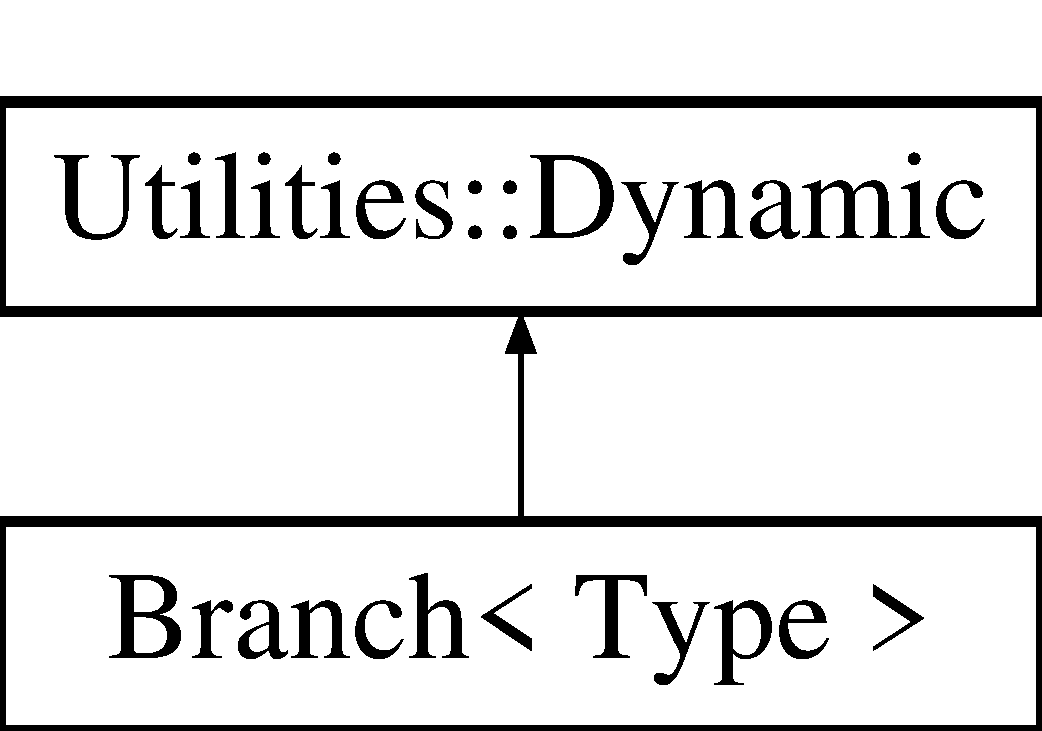
\includegraphics[height=2.000000cm]{classBranch}
\end{center}
\end{figure}
\subsection*{Public Member Functions}
\begin{DoxyCompactItemize}
\item 
\hyperlink{classBranch_aeb963f83cf85bbcdef023ddbc020a46a}{Branch} (T\+Tree $\ast$ttree, T\+String new\+\_\+branch\+\_\+name)
\item 
virtual \hyperlink{classBranch_a75022b7e676e5f675b98c1bf7922dd4e}{$\sim$\+Branch} ()
\item 
Type \hyperlink{classBranch_abe830de2e0e7c0df57fdb51436631e1e}{get\+Value} ()
\item 
void \hyperlink{classBranch_abe26b3df8dc53eeb1770d853a39865b1}{set\+Value} (Type new\+\_\+value)
\item 
void \hyperlink{classBranch_a390e9610f26ce93743237dbe3695b4c1}{set\+Reset\+Value} (Type new\+\_\+reset\+\_\+value)
\item 
void \hyperlink{classBranch_aff52fd008db1471e60107522bc62dfb7}{reset\+Value} ()
\end{DoxyCompactItemize}


\subsection{Constructor \& Destructor Documentation}
\index{Branch@{Branch}!Branch@{Branch}}
\index{Branch@{Branch}!Branch@{Branch}}
\subsubsection[{\texorpdfstring{Branch(\+T\+Tree $\ast$ttree, T\+String new\+\_\+branch\+\_\+name)}{Branch(TTree *ttree, TString new_branch_name)}}]{\setlength{\rightskip}{0pt plus 5cm}template$<$typename Type$>$ {\bf Branch}$<$ Type $>$\+::{\bf Branch} (
\begin{DoxyParamCaption}
\item[{T\+Tree $\ast$}]{ttree, }
\item[{T\+String}]{new\+\_\+branch\+\_\+name}
\end{DoxyParamCaption}
)}\hypertarget{classBranch_aeb963f83cf85bbcdef023ddbc020a46a}{}\label{classBranch_aeb963f83cf85bbcdef023ddbc020a46a}
\hyperlink{classBranch}{Branch} object constructor 
\begin{DoxyTemplParams}{Template Parameters}
{\em Type} & type of branch value \\
\hline
\end{DoxyTemplParams}

\begin{DoxyParams}{Parameters}
{\em ttree} & pointer to T\+Tree \\
\hline
{\em new\+\_\+branch\+\_\+name} & new branch name \\
\hline
\end{DoxyParams}
\begin{DoxyReturn}{Returns}
none 
\end{DoxyReturn}
\index{Branch@{Branch}!````~Branch@{$\sim$\+Branch}}
\index{````~Branch@{$\sim$\+Branch}!Branch@{Branch}}
\subsubsection[{\texorpdfstring{$\sim$\+Branch()}{~Branch()}}]{\setlength{\rightskip}{0pt plus 5cm}template$<$typename Type$>$ virtual {\bf Branch}$<$ Type $>$\+::$\sim${\bf Branch} (
\begin{DoxyParamCaption}
{}
\end{DoxyParamCaption}
)\hspace{0.3cm}{\ttfamily [virtual]}}\hypertarget{classBranch_a75022b7e676e5f675b98c1bf7922dd4e}{}\label{classBranch_a75022b7e676e5f675b98c1bf7922dd4e}
\hyperlink{classBranch}{Branch} object destructor 
\begin{DoxyTemplParams}{Template Parameters}
{\em Type} & type of branch value \\
\hline
\end{DoxyTemplParams}
\begin{DoxyReturn}{Returns}
none 
\end{DoxyReturn}


\subsection{Member Function Documentation}
\index{Branch@{Branch}!get\+Value@{get\+Value}}
\index{get\+Value@{get\+Value}!Branch@{Branch}}
\subsubsection[{\texorpdfstring{get\+Value()}{getValue()}}]{\setlength{\rightskip}{0pt plus 5cm}template$<$typename Type$>$ Type {\bf Branch}$<$ Type $>$\+::get\+Value (
\begin{DoxyParamCaption}
{}
\end{DoxyParamCaption}
)}\hypertarget{classBranch_abe830de2e0e7c0df57fdb51436631e1e}{}\label{classBranch_abe830de2e0e7c0df57fdb51436631e1e}
Get current leaf value 
\begin{DoxyTemplParams}{Template Parameters}
{\em Type} & type of branch value \\
\hline
\end{DoxyTemplParams}
\begin{DoxyReturn}{Returns}
value of current leaf 
\end{DoxyReturn}
\index{Branch@{Branch}!reset\+Value@{reset\+Value}}
\index{reset\+Value@{reset\+Value}!Branch@{Branch}}
\subsubsection[{\texorpdfstring{reset\+Value()}{resetValue()}}]{\setlength{\rightskip}{0pt plus 5cm}template$<$typename Type$>$ void {\bf Branch}$<$ Type $>$\+::reset\+Value (
\begin{DoxyParamCaption}
{}
\end{DoxyParamCaption}
)}\hypertarget{classBranch_aff52fd008db1471e60107522bc62dfb7}{}\label{classBranch_aff52fd008db1471e60107522bc62dfb7}
Reset the current leaf to the reset value 
\begin{DoxyTemplParams}{Template Parameters}
{\em Type} & type of branch value \\
\hline
\end{DoxyTemplParams}
\begin{DoxyReturn}{Returns}
none 
\end{DoxyReturn}
\index{Branch@{Branch}!set\+Reset\+Value@{set\+Reset\+Value}}
\index{set\+Reset\+Value@{set\+Reset\+Value}!Branch@{Branch}}
\subsubsection[{\texorpdfstring{set\+Reset\+Value(\+Type new\+\_\+reset\+\_\+value)}{setResetValue(Type new_reset_value)}}]{\setlength{\rightskip}{0pt plus 5cm}template$<$typename Type$>$ void {\bf Branch}$<$ Type $>$\+::set\+Reset\+Value (
\begin{DoxyParamCaption}
\item[{Type}]{new\+\_\+reset\+\_\+value}
\end{DoxyParamCaption}
)}\hypertarget{classBranch_a390e9610f26ce93743237dbe3695b4c1}{}\label{classBranch_a390e9610f26ce93743237dbe3695b4c1}
Set the reset value of branch 
\begin{DoxyTemplParams}{Template Parameters}
{\em Type} & type of branch value \\
\hline
\end{DoxyTemplParams}

\begin{DoxyParams}{Parameters}
{\em new\+\_\+reset\+\_\+value} & new reset value (e.\+g. -\/999; default is the default type constructor) \\
\hline
\end{DoxyParams}
\begin{DoxyReturn}{Returns}
none 
\end{DoxyReturn}
\index{Branch@{Branch}!set\+Value@{set\+Value}}
\index{set\+Value@{set\+Value}!Branch@{Branch}}
\subsubsection[{\texorpdfstring{set\+Value(\+Type new\+\_\+value)}{setValue(Type new_value)}}]{\setlength{\rightskip}{0pt plus 5cm}template$<$typename Type$>$ void {\bf Branch}$<$ Type $>$\+::set\+Value (
\begin{DoxyParamCaption}
\item[{Type}]{new\+\_\+value}
\end{DoxyParamCaption}
)}\hypertarget{classBranch_abe26b3df8dc53eeb1770d853a39865b1}{}\label{classBranch_abe26b3df8dc53eeb1770d853a39865b1}
Set value of current leaf 
\begin{DoxyTemplParams}{Template Parameters}
{\em Type} & type of branch value \\
\hline
\end{DoxyTemplParams}

\begin{DoxyParams}{Parameters}
{\em new\+\_\+value} & new value \\
\hline
\end{DoxyParams}
\begin{DoxyReturn}{Returns}
none 
\end{DoxyReturn}


The documentation for this class was generated from the following file\+:\begin{DoxyCompactItemize}
\item 
arbol.\+h\end{DoxyCompactItemize}

\hypertarget{classUtilities_1_1CSVFile}{}\doxysection{Utilities\+::CSVFile Class Reference}
\label{classUtilities_1_1CSVFile}\index{Utilities::CSVFile@{Utilities::CSVFile}}


{\ttfamily \#include $<$utilities.\+h$>$}

\doxysubsection*{Public Member Functions}
\begin{DoxyCompactItemize}
\item 
\mbox{\hyperlink{classUtilities_1_1CSVFile_a35c6dd1a71618229cdd5f5e1ca6de4e9}{CSVFile}} (std\+::ofstream \&new\+\_\+ofstream, std\+::string new\+\_\+name, std\+::vector$<$ std\+::string $>$ new\+\_\+headers)
\item 
virtual \mbox{\hyperlink{classUtilities_1_1CSVFile_a4e90ae7fd8a4de6908aab2554eac76d0}{$\sim$\+CSVFile}} ()
\item 
\mbox{\hyperlink{classUtilities_1_1CSVFile}{CSVFile}} \mbox{\hyperlink{classUtilities_1_1CSVFile_a7394abaf33c2cf1bc557bba58cf0e453}{clone}} (std\+::string new\+\_\+name)
\item 
{\footnotesize template$<$typename Type $>$ }\\void \mbox{\hyperlink{classUtilities_1_1CSVFile_ad0fc6d028ca1010f6597fa9a18f3db7a}{push\+Col}} (Type value)
\item 
void \mbox{\hyperlink{classUtilities_1_1CSVFile_a592fc96c51382efb35c6708acbfa69c2}{write\+Row}} (bool append=true)
\end{DoxyCompactItemize}
\doxysubsection*{Public Attributes}
\begin{DoxyCompactItemize}
\item 
std\+::ofstream \& \mbox{\hyperlink{classUtilities_1_1CSVFile_a3ceb6ad218bb1e729b03a51e326fc12b}{ofstream}}
\item 
std\+::string \mbox{\hyperlink{classUtilities_1_1CSVFile_a26f01db1cc36f242adf00b17b4f63e37}{name}}
\item 
std\+::vector$<$ std\+::string $>$ \mbox{\hyperlink{classUtilities_1_1CSVFile_a17822ae335f168e68498b8b1b69b8dbe}{headers}}
\item 
std\+::vector$<$ std\+::string $>$ \mbox{\hyperlink{classUtilities_1_1CSVFile_aa1ab5bfb37837aaba9b6cabd38c96bb3}{buffer}}
\end{DoxyCompactItemize}


\doxysubsection{Detailed Description}
Object for handling CSV I/O 

\doxysubsection{Constructor \& Destructor Documentation}
\mbox{\Hypertarget{classUtilities_1_1CSVFile_a35c6dd1a71618229cdd5f5e1ca6de4e9}\label{classUtilities_1_1CSVFile_a35c6dd1a71618229cdd5f5e1ca6de4e9}} 
\index{Utilities::CSVFile@{Utilities::CSVFile}!CSVFile@{CSVFile}}
\index{CSVFile@{CSVFile}!Utilities::CSVFile@{Utilities::CSVFile}}
\doxysubsubsection{\texorpdfstring{CSVFile()}{CSVFile()}}
{\footnotesize\ttfamily Utilities\+::\+CSVFile\+::\+CSVFile (\begin{DoxyParamCaption}\item[{std\+::ofstream \&}]{new\+\_\+ofstream,  }\item[{std\+::string}]{new\+\_\+name,  }\item[{std\+::vector$<$ std\+::string $>$}]{new\+\_\+headers }\end{DoxyParamCaption})}

\mbox{\hyperlink{classUtilities_1_1CSVFile}{CSVFile}} object constructor 
\begin{DoxyParams}{Parameters}
{\em new\+\_\+ofstream} & reference of an existing ofstream object \\
\hline
{\em new\+\_\+name} & name of new CSV file (e.\+g. output.\+csv) \\
\hline
{\em new\+\_\+headers} & headers for new CSV file columns \\
\hline
\end{DoxyParams}
\begin{DoxyReturn}{Returns}
none 
\end{DoxyReturn}
\mbox{\Hypertarget{classUtilities_1_1CSVFile_a4e90ae7fd8a4de6908aab2554eac76d0}\label{classUtilities_1_1CSVFile_a4e90ae7fd8a4de6908aab2554eac76d0}} 
\index{Utilities::CSVFile@{Utilities::CSVFile}!````~CSVFile@{$\sim$CSVFile}}
\index{````~CSVFile@{$\sim$CSVFile}!Utilities::CSVFile@{Utilities::CSVFile}}
\doxysubsubsection{\texorpdfstring{$\sim$CSVFile()}{~CSVFile()}}
{\footnotesize\ttfamily virtual Utilities\+::\+CSVFile\+::$\sim$\+CSVFile (\begin{DoxyParamCaption}{ }\end{DoxyParamCaption})\hspace{0.3cm}{\ttfamily [virtual]}}

\mbox{\hyperlink{classUtilities_1_1CSVFile}{CSVFile}} object destructor \begin{DoxyReturn}{Returns}
none 
\end{DoxyReturn}


\doxysubsection{Member Function Documentation}
\mbox{\Hypertarget{classUtilities_1_1CSVFile_a7394abaf33c2cf1bc557bba58cf0e453}\label{classUtilities_1_1CSVFile_a7394abaf33c2cf1bc557bba58cf0e453}} 
\index{Utilities::CSVFile@{Utilities::CSVFile}!clone@{clone}}
\index{clone@{clone}!Utilities::CSVFile@{Utilities::CSVFile}}
\doxysubsubsection{\texorpdfstring{clone()}{clone()}}
{\footnotesize\ttfamily \mbox{\hyperlink{classUtilities_1_1CSVFile}{CSVFile}} Utilities\+::\+CSVFile\+::clone (\begin{DoxyParamCaption}\item[{std\+::string}]{new\+\_\+name }\end{DoxyParamCaption})}

Clone \mbox{\hyperlink{classUtilities_1_1CSVFile}{CSVFile}} object and copy the existing CSV file to a new file 
\begin{DoxyParams}{Parameters}
{\em new\+\_\+name} & name of new CSV file (e.\+g. output.\+csv) \\
\hline
\end{DoxyParams}
\begin{DoxyReturn}{Returns}
new \mbox{\hyperlink{classUtilities_1_1CSVFile}{CSVFile}} object 
\end{DoxyReturn}
\mbox{\Hypertarget{classUtilities_1_1CSVFile_ad0fc6d028ca1010f6597fa9a18f3db7a}\label{classUtilities_1_1CSVFile_ad0fc6d028ca1010f6597fa9a18f3db7a}} 
\index{Utilities::CSVFile@{Utilities::CSVFile}!pushCol@{pushCol}}
\index{pushCol@{pushCol}!Utilities::CSVFile@{Utilities::CSVFile}}
\doxysubsubsection{\texorpdfstring{pushCol()}{pushCol()}}
{\footnotesize\ttfamily template$<$typename Type $>$ \\
void Utilities\+::\+CSVFile\+::push\+Col (\begin{DoxyParamCaption}\item[{Type}]{value }\end{DoxyParamCaption})}

Push a new column entry to buffer 
\begin{DoxyTemplParams}{Template Parameters}
{\em Type} & type of column entry \\
\hline
\end{DoxyTemplParams}

\begin{DoxyParams}{Parameters}
{\em value} & new column entry \\
\hline
\end{DoxyParams}
\begin{DoxyReturn}{Returns}
none 
\end{DoxyReturn}
\mbox{\Hypertarget{classUtilities_1_1CSVFile_a592fc96c51382efb35c6708acbfa69c2}\label{classUtilities_1_1CSVFile_a592fc96c51382efb35c6708acbfa69c2}} 
\index{Utilities::CSVFile@{Utilities::CSVFile}!writeRow@{writeRow}}
\index{writeRow@{writeRow}!Utilities::CSVFile@{Utilities::CSVFile}}
\doxysubsubsection{\texorpdfstring{writeRow()}{writeRow()}}
{\footnotesize\ttfamily void Utilities\+::\+CSVFile\+::write\+Row (\begin{DoxyParamCaption}\item[{bool}]{append = {\ttfamily true} }\end{DoxyParamCaption})}

Write buffer to CSV file 
\begin{DoxyParams}{Parameters}
{\em append} & Toggle \char`\"{}append\char`\"{} mode (optional) \\
\hline
\end{DoxyParams}
\begin{DoxyReturn}{Returns}
none 
\end{DoxyReturn}


\doxysubsection{Member Data Documentation}
\mbox{\Hypertarget{classUtilities_1_1CSVFile_aa1ab5bfb37837aaba9b6cabd38c96bb3}\label{classUtilities_1_1CSVFile_aa1ab5bfb37837aaba9b6cabd38c96bb3}} 
\index{Utilities::CSVFile@{Utilities::CSVFile}!buffer@{buffer}}
\index{buffer@{buffer}!Utilities::CSVFile@{Utilities::CSVFile}}
\doxysubsubsection{\texorpdfstring{buffer}{buffer}}
{\footnotesize\ttfamily std\+::vector$<$std\+::string$>$ Utilities\+::\+CSVFile\+::buffer}

Buffer for staging column values \mbox{\Hypertarget{classUtilities_1_1CSVFile_a17822ae335f168e68498b8b1b69b8dbe}\label{classUtilities_1_1CSVFile_a17822ae335f168e68498b8b1b69b8dbe}} 
\index{Utilities::CSVFile@{Utilities::CSVFile}!headers@{headers}}
\index{headers@{headers}!Utilities::CSVFile@{Utilities::CSVFile}}
\doxysubsubsection{\texorpdfstring{headers}{headers}}
{\footnotesize\ttfamily std\+::vector$<$std\+::string$>$ Utilities\+::\+CSVFile\+::headers}

Headers for CSV columns \mbox{\Hypertarget{classUtilities_1_1CSVFile_a26f01db1cc36f242adf00b17b4f63e37}\label{classUtilities_1_1CSVFile_a26f01db1cc36f242adf00b17b4f63e37}} 
\index{Utilities::CSVFile@{Utilities::CSVFile}!name@{name}}
\index{name@{name}!Utilities::CSVFile@{Utilities::CSVFile}}
\doxysubsubsection{\texorpdfstring{name}{name}}
{\footnotesize\ttfamily std\+::string Utilities\+::\+CSVFile\+::name}

Name (e.\+g. output.\+csv) of CSV file \mbox{\Hypertarget{classUtilities_1_1CSVFile_a3ceb6ad218bb1e729b03a51e326fc12b}\label{classUtilities_1_1CSVFile_a3ceb6ad218bb1e729b03a51e326fc12b}} 
\index{Utilities::CSVFile@{Utilities::CSVFile}!ofstream@{ofstream}}
\index{ofstream@{ofstream}!Utilities::CSVFile@{Utilities::CSVFile}}
\doxysubsubsection{\texorpdfstring{ofstream}{ofstream}}
{\footnotesize\ttfamily std\+::ofstream\& Utilities\+::\+CSVFile\+::ofstream}

fstream object for writing files 

The documentation for this class was generated from the following file\+:\begin{DoxyCompactItemize}
\item 
utilities.\+h\end{DoxyCompactItemize}

\hypertarget{classCut}{}\doxysection{Cut Class Reference}
\label{classCut}\index{Cut@{Cut}}


{\ttfamily \#include $<$cutflow.\+h$>$}

\doxysubsection*{Public Member Functions}
\begin{DoxyCompactItemize}
\item 
\mbox{\hyperlink{classCut_aaa89435c5326080296041bc38937ab2d}{Cut}} (std\+::string new\+\_\+name, std\+::function$<$ bool()$>$ new\+\_\+evaluate)
\item 
\mbox{\hyperlink{classCut_adcfec6d2df97f8e84058078f2f736b03}{Cut}} (std\+::string new\+\_\+name, std\+::function$<$ bool()$>$ new\+\_\+evaluate, std\+::function$<$ float()$>$ new\+\_\+compute\+\_\+weight)
\item 
\mbox{\hyperlink{classCut}{Cut}} $\ast$ \mbox{\hyperlink{classCut_a51d128a9d77f6e9e2965ae0a2ea077e1}{clone}} (std\+::string new\+\_\+name)
\item 
void \mbox{\hyperlink{classCut_a9b1298219ed1f85bba920e4049d712e3}{print}} ()
\item 
float \mbox{\hyperlink{classCut_a3201e86949718110994a9301987f0f98}{get\+Weight}} ()
\end{DoxyCompactItemize}
\doxysubsection*{Public Attributes}
\begin{DoxyCompactItemize}
\item 
std\+::string \mbox{\hyperlink{classCut_accf700d2d00746b97a265d4aea3f55c2}{name}}
\item 
std\+::function$<$ bool()$>$ \mbox{\hyperlink{classCut_a4205ad5e62b859536797141f3ace2253}{evaluate}}
\item 
std\+::function$<$ float()$>$ \mbox{\hyperlink{classCut_a908dfdeed9d882ca026427c0942fb999}{compute\+\_\+weight}}
\item 
\mbox{\hyperlink{classCut}{Cut}} $\ast$ \mbox{\hyperlink{classCut_acb046f96bc50db055cccdb1f9a601780}{parent}}
\item 
\mbox{\hyperlink{classCut}{Cut}} $\ast$ \mbox{\hyperlink{classCut_a2142ffe68028bb0c211408c0f5bb8bfb}{right}}
\item 
\mbox{\hyperlink{classCut}{Cut}} $\ast$ \mbox{\hyperlink{classCut_a2c65e372172dfa0f705d117d3ad0f668}{left}}
\item 
int \mbox{\hyperlink{classCut_a01ab47c909e962b3820e2e866c0230a8}{n\+\_\+pass}}
\item 
int \mbox{\hyperlink{classCut_aff7fd0749654bdae7ede4bfbea700c2d}{n\+\_\+fail}}
\item 
float \mbox{\hyperlink{classCut_ac5f58e08d36bad07f9c62ab9c04eb1b7}{n\+\_\+pass\+\_\+weighted}}
\item 
float \mbox{\hyperlink{classCut_ad780ce231646c09c612b14180b2772e0}{n\+\_\+fail\+\_\+weighted}}
\end{DoxyCompactItemize}


\doxysubsection{Detailed Description}
Object that represents a single cut in an analysis 

\doxysubsection{Constructor \& Destructor Documentation}
\mbox{\Hypertarget{classCut_aaa89435c5326080296041bc38937ab2d}\label{classCut_aaa89435c5326080296041bc38937ab2d}} 
\index{Cut@{Cut}!Cut@{Cut}}
\index{Cut@{Cut}!Cut@{Cut}}
\doxysubsubsection{\texorpdfstring{Cut()}{Cut()}\hspace{0.1cm}{\footnotesize\ttfamily [1/2]}}
{\footnotesize\ttfamily Cut\+::\+Cut (\begin{DoxyParamCaption}\item[{std\+::string}]{new\+\_\+name,  }\item[{std\+::function$<$ bool()$>$}]{new\+\_\+evaluate }\end{DoxyParamCaption})}

\mbox{\hyperlink{classCut}{Cut}} object constructor (assumes weight == 1.\+0) 
\begin{DoxyParams}{Parameters}
{\em new\+\_\+name} & new cut name \\
\hline
{\em new\+\_\+evaluate} & lambda function that evaluates new cut conditional logic \\
\hline
\end{DoxyParams}
\begin{DoxyReturn}{Returns}
none 
\end{DoxyReturn}
\mbox{\Hypertarget{classCut_adcfec6d2df97f8e84058078f2f736b03}\label{classCut_adcfec6d2df97f8e84058078f2f736b03}} 
\index{Cut@{Cut}!Cut@{Cut}}
\index{Cut@{Cut}!Cut@{Cut}}
\doxysubsubsection{\texorpdfstring{Cut()}{Cut()}\hspace{0.1cm}{\footnotesize\ttfamily [2/2]}}
{\footnotesize\ttfamily Cut\+::\+Cut (\begin{DoxyParamCaption}\item[{std\+::string}]{new\+\_\+name,  }\item[{std\+::function$<$ bool()$>$}]{new\+\_\+evaluate,  }\item[{std\+::function$<$ float()$>$}]{new\+\_\+compute\+\_\+weight }\end{DoxyParamCaption})}

\mbox{\hyperlink{classCut}{Cut}} object constructor 
\begin{DoxyParams}{Parameters}
{\em new\+\_\+name} & new cut name \\
\hline
{\em new\+\_\+evaluate} & lambda function that evaluates new cut conditional logic \\
\hline
{\em new\+\_\+compute\+\_\+weight} & lambda function that computes event weight \\
\hline
\end{DoxyParams}
\begin{DoxyReturn}{Returns}
none 
\end{DoxyReturn}


\doxysubsection{Member Function Documentation}
\mbox{\Hypertarget{classCut_a51d128a9d77f6e9e2965ae0a2ea077e1}\label{classCut_a51d128a9d77f6e9e2965ae0a2ea077e1}} 
\index{Cut@{Cut}!clone@{clone}}
\index{clone@{clone}!Cut@{Cut}}
\doxysubsubsection{\texorpdfstring{clone()}{clone()}}
{\footnotesize\ttfamily \mbox{\hyperlink{classCut}{Cut}} $\ast$ Cut\+::clone (\begin{DoxyParamCaption}\item[{std\+::string}]{new\+\_\+name }\end{DoxyParamCaption})}

Create a copy of this cut object 
\begin{DoxyParams}{Parameters}
{\em new\+\_\+name} & name of cut copy \\
\hline
\end{DoxyParams}
\begin{DoxyReturn}{Returns}
pointer to a copy of this cut object 
\end{DoxyReturn}
\mbox{\Hypertarget{classCut_a3201e86949718110994a9301987f0f98}\label{classCut_a3201e86949718110994a9301987f0f98}} 
\index{Cut@{Cut}!getWeight@{getWeight}}
\index{getWeight@{getWeight}!Cut@{Cut}}
\doxysubsubsection{\texorpdfstring{getWeight()}{getWeight()}}
{\footnotesize\ttfamily float Cut\+::get\+Weight (\begin{DoxyParamCaption}{ }\end{DoxyParamCaption})}

Get even weight for this cut (on top of previous cut weights) \begin{DoxyReturn}{Returns}
event weight 
\end{DoxyReturn}
\mbox{\Hypertarget{classCut_a9b1298219ed1f85bba920e4049d712e3}\label{classCut_a9b1298219ed1f85bba920e4049d712e3}} 
\index{Cut@{Cut}!print@{print}}
\index{print@{print}!Cut@{Cut}}
\doxysubsubsection{\texorpdfstring{print()}{print()}}
{\footnotesize\ttfamily void Cut\+::print (\begin{DoxyParamCaption}{ }\end{DoxyParamCaption})}

Print cut object properties \begin{DoxyReturn}{Returns}
none 
\end{DoxyReturn}


\doxysubsection{Member Data Documentation}
\mbox{\Hypertarget{classCut_a908dfdeed9d882ca026427c0942fb999}\label{classCut_a908dfdeed9d882ca026427c0942fb999}} 
\index{Cut@{Cut}!compute\_weight@{compute\_weight}}
\index{compute\_weight@{compute\_weight}!Cut@{Cut}}
\doxysubsubsection{\texorpdfstring{compute\_weight}{compute\_weight}}
{\footnotesize\ttfamily std\+::function$<$float()$>$ Cut\+::compute\+\_\+weight}

Lambda function that computes event weight \mbox{\Hypertarget{classCut_a4205ad5e62b859536797141f3ace2253}\label{classCut_a4205ad5e62b859536797141f3ace2253}} 
\index{Cut@{Cut}!evaluate@{evaluate}}
\index{evaluate@{evaluate}!Cut@{Cut}}
\doxysubsubsection{\texorpdfstring{evaluate}{evaluate}}
{\footnotesize\ttfamily std\+::function$<$bool()$>$ Cut\+::evaluate}

Lambda function that evaluates conditional logic (i.\+e. the cut itself) \mbox{\Hypertarget{classCut_a2c65e372172dfa0f705d117d3ad0f668}\label{classCut_a2c65e372172dfa0f705d117d3ad0f668}} 
\index{Cut@{Cut}!left@{left}}
\index{left@{left}!Cut@{Cut}}
\doxysubsubsection{\texorpdfstring{left}{left}}
{\footnotesize\ttfamily \mbox{\hyperlink{classCut}{Cut}}$\ast$ Cut\+::left}

Pointer to next cut to evaluate if this cut evaluates to false \mbox{\Hypertarget{classCut_aff7fd0749654bdae7ede4bfbea700c2d}\label{classCut_aff7fd0749654bdae7ede4bfbea700c2d}} 
\index{Cut@{Cut}!n\_fail@{n\_fail}}
\index{n\_fail@{n\_fail}!Cut@{Cut}}
\doxysubsubsection{\texorpdfstring{n\_fail}{n\_fail}}
{\footnotesize\ttfamily int Cut\+::n\+\_\+fail}

Number of events that fail cut \mbox{\Hypertarget{classCut_ad780ce231646c09c612b14180b2772e0}\label{classCut_ad780ce231646c09c612b14180b2772e0}} 
\index{Cut@{Cut}!n\_fail\_weighted@{n\_fail\_weighted}}
\index{n\_fail\_weighted@{n\_fail\_weighted}!Cut@{Cut}}
\doxysubsubsection{\texorpdfstring{n\_fail\_weighted}{n\_fail\_weighted}}
{\footnotesize\ttfamily float Cut\+::n\+\_\+fail\+\_\+weighted}

Weighted number of events that fail cut \mbox{\Hypertarget{classCut_a01ab47c909e962b3820e2e866c0230a8}\label{classCut_a01ab47c909e962b3820e2e866c0230a8}} 
\index{Cut@{Cut}!n\_pass@{n\_pass}}
\index{n\_pass@{n\_pass}!Cut@{Cut}}
\doxysubsubsection{\texorpdfstring{n\_pass}{n\_pass}}
{\footnotesize\ttfamily int Cut\+::n\+\_\+pass}

Number of events that pass cut \mbox{\Hypertarget{classCut_ac5f58e08d36bad07f9c62ab9c04eb1b7}\label{classCut_ac5f58e08d36bad07f9c62ab9c04eb1b7}} 
\index{Cut@{Cut}!n\_pass\_weighted@{n\_pass\_weighted}}
\index{n\_pass\_weighted@{n\_pass\_weighted}!Cut@{Cut}}
\doxysubsubsection{\texorpdfstring{n\_pass\_weighted}{n\_pass\_weighted}}
{\footnotesize\ttfamily float Cut\+::n\+\_\+pass\+\_\+weighted}

Weighted number of events that pass cut \mbox{\Hypertarget{classCut_accf700d2d00746b97a265d4aea3f55c2}\label{classCut_accf700d2d00746b97a265d4aea3f55c2}} 
\index{Cut@{Cut}!name@{name}}
\index{name@{name}!Cut@{Cut}}
\doxysubsubsection{\texorpdfstring{name}{name}}
{\footnotesize\ttfamily std\+::string Cut\+::name}

Unique name of cut \mbox{\Hypertarget{classCut_acb046f96bc50db055cccdb1f9a601780}\label{classCut_acb046f96bc50db055cccdb1f9a601780}} 
\index{Cut@{Cut}!parent@{parent}}
\index{parent@{parent}!Cut@{Cut}}
\doxysubsubsection{\texorpdfstring{parent}{parent}}
{\footnotesize\ttfamily \mbox{\hyperlink{classCut}{Cut}}$\ast$ Cut\+::parent}

Pointer to parent cut \mbox{\Hypertarget{classCut_a2142ffe68028bb0c211408c0f5bb8bfb}\label{classCut_a2142ffe68028bb0c211408c0f5bb8bfb}} 
\index{Cut@{Cut}!right@{right}}
\index{right@{right}!Cut@{Cut}}
\doxysubsubsection{\texorpdfstring{right}{right}}
{\footnotesize\ttfamily \mbox{\hyperlink{classCut}{Cut}}$\ast$ Cut\+::right}

Pointer to next cut to evaluate if this cut evaluates to true 

The documentation for this class was generated from the following files\+:\begin{DoxyCompactItemize}
\item 
/github/workspace/rapido/src/cutflow.\+h\item 
/github/workspace/rapido/src/cutflow.\+cc\end{DoxyCompactItemize}

\hypertarget{classCutflow}{}\doxysection{Cutflow Class Reference}
\label{classCutflow}\index{Cutflow@{Cutflow}}


{\ttfamily \#include $<$cutflow.\+h$>$}

Inheritance diagram for Cutflow\+:\begin{figure}[H]
\begin{center}
\leavevmode
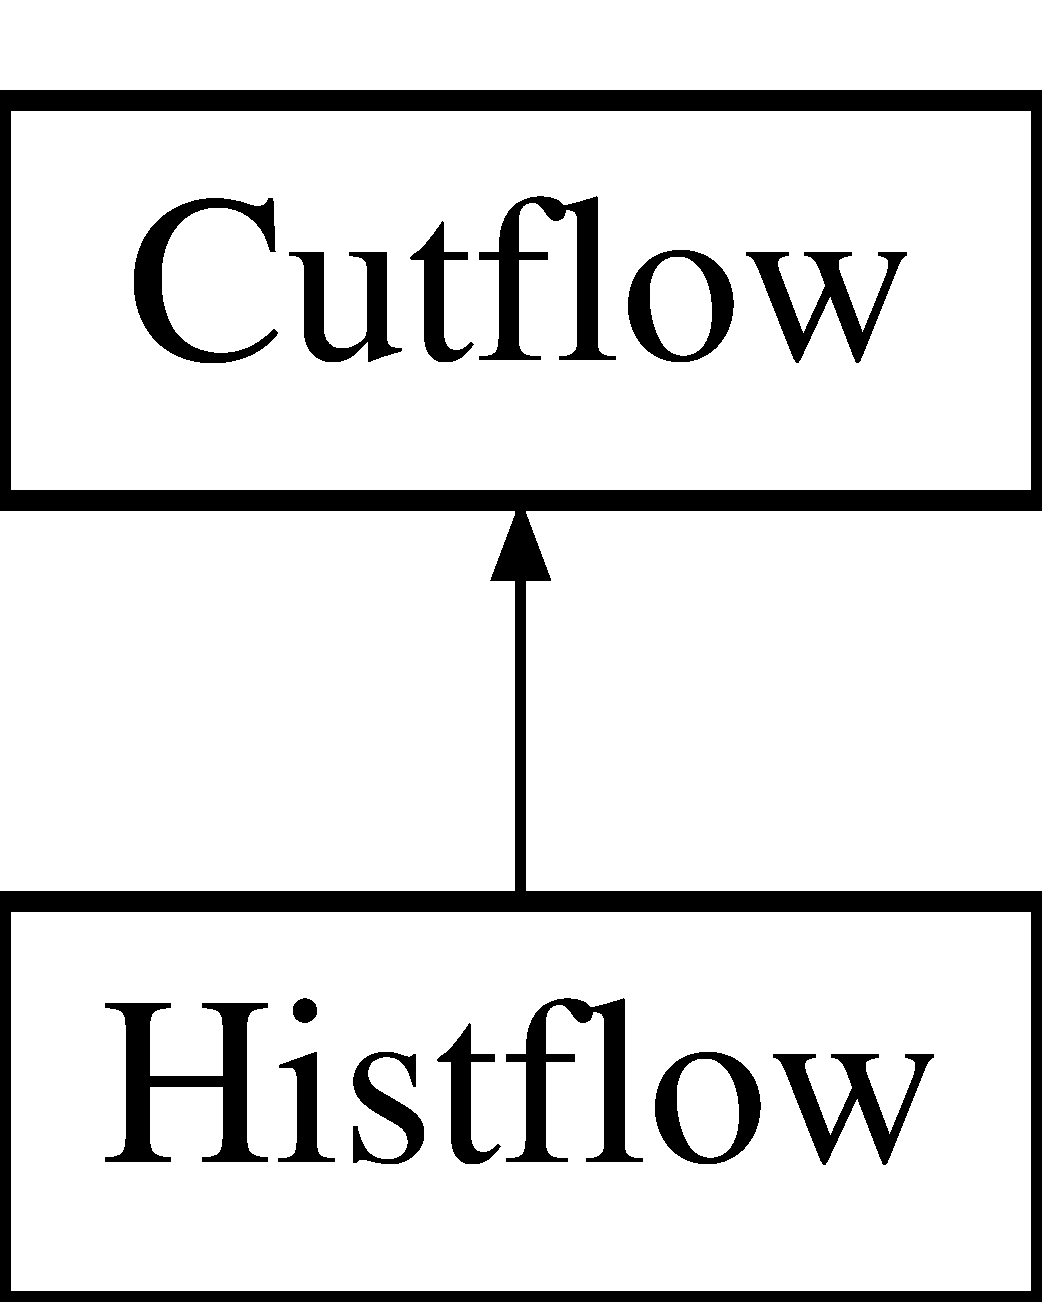
\includegraphics[height=2.000000cm]{classCutflow}
\end{center}
\end{figure}
\doxysubsection*{Public Member Functions}
\begin{DoxyCompactItemize}
\item 
\mbox{\hyperlink{classCutflow_a17811cb40a7906fc65e79ce69e3b21be}{Cutflow}} ()
\item 
\mbox{\hyperlink{classCutflow_a46b6444272c54fe9988e8d328d0644ca}{Cutflow}} (std\+::string new\+\_\+name)
\item 
\mbox{\hyperlink{classCutflow_ae13ef13d8c6cef09bed242855e45aacf}{Cutflow}} (std\+::string new\+\_\+name, \mbox{\hyperlink{classCut}{Cut}} $\ast$new\+\_\+root)
\item 
\mbox{\hyperlink{classCutflow_adb300cd78d57a287934e4d22856a0ffe}{$\sim$\+Cutflow}} ()
\item 
void \mbox{\hyperlink{classCutflow_ad27d37141c3748779a5d81fad919ecbb}{set\+Root}} (\mbox{\hyperlink{classCut}{Cut}} $\ast$new\+\_\+root)
\item 
void \mbox{\hyperlink{classCutflow_a8da46f1053a6b97991489ee0920c29a1}{insert}} (std\+::string target\+\_\+cut\+\_\+name, \mbox{\hyperlink{classCut}{Cut}} $\ast$new\+\_\+cut, Direction direction)
\item 
virtual bool \mbox{\hyperlink{classCutflow_a8fc98b9c006b80db96576c8bdcf6a0a8}{run}} ()
\item 
bool \mbox{\hyperlink{classCutflow_a3b5a6dc6e9490037d190eca691295859}{run\+Until}} (std\+::string target\+\_\+cut\+\_\+name)
\item 
\mbox{\hyperlink{classCut}{Cut}} $\ast$ \mbox{\hyperlink{classCutflow_a11c1116dc01d4c0679945eeff66ff0a4}{find\+Terminus}} (std\+::string starting\+\_\+cut\+\_\+name)
\item 
void \mbox{\hyperlink{classCutflow_a0cb4c8bd6d15ace1f85fe0cfb8d9d828}{print}} ()
\item 
void \mbox{\hyperlink{classCutflow_a43e58326fbce5306e2b3d080c6cd85f0}{write\+CSV}} (std\+::string output\+\_\+dir=\char`\"{}\char`\"{})
\end{DoxyCompactItemize}
\doxysubsection*{Public Attributes}
\begin{DoxyCompactItemize}
\item 
std\+::string \mbox{\hyperlink{classCutflow_a268e204c942ca35895a94f1be7ce111d}{name}}
\item 
\mbox{\hyperlink{classUtilities_1_1Variables}{Utilities\+::\+Variables}} \mbox{\hyperlink{classCutflow_a71390324488ac6ed4a72c41f4a2c1c10}{globals}}
\end{DoxyCompactItemize}
\doxysubsection*{Protected Member Functions}
\begin{DoxyCompactItemize}
\item 
\mbox{\hyperlink{classCut}{Cut}} $\ast$ \mbox{\hyperlink{classCutflow_a20193ee89ee39b0fc58ab4f27e2779db}{get\+Cut}} (std\+::string cut\+\_\+name)
\item 
\mbox{\hyperlink{classCut}{Cut}} $\ast$ \mbox{\hyperlink{classCutflow_a6949f1d9e7d74c6ab8cf0c6f28ac3701}{recursive\+Find\+Terminus}} (\mbox{\hyperlink{classCut}{Cut}} $\ast$cut)
\item 
void \mbox{\hyperlink{classCutflow_a54e6ae7d3e4c9efdb8fd830ab8a0e0e9}{recursive\+Print}} (std\+::string tabs, \mbox{\hyperlink{classCut}{Cut}} $\ast$cut, Direction direction, float weight)
\item 
std\+::pair$<$ \mbox{\hyperlink{classCut}{Cut}} $\ast$, bool $>$ \mbox{\hyperlink{classCutflow_a8298a5ed45d1963271dbe9c7d1f1586f}{recursive\+Evaluate}} (\mbox{\hyperlink{classCut}{Cut}} $\ast$cut)
\item 
void \mbox{\hyperlink{classCutflow_adc7029b27ff8d742d10c75d6f6342dac}{recursive\+Delete}} (\mbox{\hyperlink{classCut}{Cut}} $\ast$cut)
\end{DoxyCompactItemize}
\doxysubsection*{Protected Attributes}
\begin{DoxyCompactItemize}
\item 
\mbox{\hyperlink{classCut}{Cut}} $\ast$ \mbox{\hyperlink{classCutflow_a96f2343bfae77c94f2e87b5f3a128d6d}{root}}
\item 
std\+::map$<$ std\+::string, \mbox{\hyperlink{classCut}{Cut}} $\ast$ $>$ \mbox{\hyperlink{classCutflow_a76f5cbd82750844d379384c7b1243cca}{cut\+\_\+record}}
\end{DoxyCompactItemize}


\doxysubsection{Detailed Description}
An analysis represented as a binary search tree (i.\+e. analysis = tree, cut = node) 

\doxysubsection{Constructor \& Destructor Documentation}
\mbox{\Hypertarget{classCutflow_a17811cb40a7906fc65e79ce69e3b21be}\label{classCutflow_a17811cb40a7906fc65e79ce69e3b21be}} 
\index{Cutflow@{Cutflow}!Cutflow@{Cutflow}}
\index{Cutflow@{Cutflow}!Cutflow@{Cutflow}}
\doxysubsubsection{\texorpdfstring{Cutflow()}{Cutflow()}\hspace{0.1cm}{\footnotesize\ttfamily [1/3]}}
{\footnotesize\ttfamily Cutflow\+::\+Cutflow (\begin{DoxyParamCaption}{ }\end{DoxyParamCaption})}

\mbox{\hyperlink{classCutflow}{Cutflow}} object default constructor \begin{DoxyReturn}{Returns}
none 
\end{DoxyReturn}
\mbox{\Hypertarget{classCutflow_a46b6444272c54fe9988e8d328d0644ca}\label{classCutflow_a46b6444272c54fe9988e8d328d0644ca}} 
\index{Cutflow@{Cutflow}!Cutflow@{Cutflow}}
\index{Cutflow@{Cutflow}!Cutflow@{Cutflow}}
\doxysubsubsection{\texorpdfstring{Cutflow()}{Cutflow()}\hspace{0.1cm}{\footnotesize\ttfamily [2/3]}}
{\footnotesize\ttfamily Cutflow\+::\+Cutflow (\begin{DoxyParamCaption}\item[{std\+::string}]{new\+\_\+name }\end{DoxyParamCaption})}

\mbox{\hyperlink{classCutflow}{Cutflow}} object overload constructor 
\begin{DoxyParams}{Parameters}
{\em new\+\_\+name} & name of cutflow \\
\hline
\end{DoxyParams}
\begin{DoxyReturn}{Returns}
none 
\end{DoxyReturn}
\mbox{\Hypertarget{classCutflow_ae13ef13d8c6cef09bed242855e45aacf}\label{classCutflow_ae13ef13d8c6cef09bed242855e45aacf}} 
\index{Cutflow@{Cutflow}!Cutflow@{Cutflow}}
\index{Cutflow@{Cutflow}!Cutflow@{Cutflow}}
\doxysubsubsection{\texorpdfstring{Cutflow()}{Cutflow()}\hspace{0.1cm}{\footnotesize\ttfamily [3/3]}}
{\footnotesize\ttfamily Cutflow\+::\+Cutflow (\begin{DoxyParamCaption}\item[{std\+::string}]{new\+\_\+name,  }\item[{\mbox{\hyperlink{classCut}{Cut}} $\ast$}]{new\+\_\+root }\end{DoxyParamCaption})}

\mbox{\hyperlink{classCutflow}{Cutflow}} object overload constructor 
\begin{DoxyParams}{Parameters}
{\em new\+\_\+name} & name of cutflow \\
\hline
{\em new\+\_\+root} & pointer to cut object to use as root node \\
\hline
\end{DoxyParams}
\begin{DoxyReturn}{Returns}
none 
\end{DoxyReturn}
\mbox{\Hypertarget{classCutflow_adb300cd78d57a287934e4d22856a0ffe}\label{classCutflow_adb300cd78d57a287934e4d22856a0ffe}} 
\index{Cutflow@{Cutflow}!````~Cutflow@{$\sim$Cutflow}}
\index{````~Cutflow@{$\sim$Cutflow}!Cutflow@{Cutflow}}
\doxysubsubsection{\texorpdfstring{$\sim$Cutflow()}{~Cutflow()}}
{\footnotesize\ttfamily Cutflow\+::$\sim$\+Cutflow (\begin{DoxyParamCaption}{ }\end{DoxyParamCaption})}

\mbox{\hyperlink{classCutflow}{Cutflow}} object destructor \begin{DoxyReturn}{Returns}
none 
\end{DoxyReturn}


\doxysubsection{Member Function Documentation}
\mbox{\Hypertarget{classCutflow_a11c1116dc01d4c0679945eeff66ff0a4}\label{classCutflow_a11c1116dc01d4c0679945eeff66ff0a4}} 
\index{Cutflow@{Cutflow}!findTerminus@{findTerminus}}
\index{findTerminus@{findTerminus}!Cutflow@{Cutflow}}
\doxysubsubsection{\texorpdfstring{findTerminus()}{findTerminus()}}
{\footnotesize\ttfamily \mbox{\hyperlink{classCut}{Cut}} $\ast$ Cutflow\+::find\+Terminus (\begin{DoxyParamCaption}\item[{std\+::string}]{starting\+\_\+cut\+\_\+name }\end{DoxyParamCaption})}

Find the rightmost terminal leaf from a given node 
\begin{DoxyParams}{Parameters}
{\em starting\+\_\+cut\+\_\+name} & cut from which to start search \\
\hline
\end{DoxyParams}
\begin{DoxyReturn}{Returns}
terminal cut 
\end{DoxyReturn}
\mbox{\Hypertarget{classCutflow_a20193ee89ee39b0fc58ab4f27e2779db}\label{classCutflow_a20193ee89ee39b0fc58ab4f27e2779db}} 
\index{Cutflow@{Cutflow}!getCut@{getCut}}
\index{getCut@{getCut}!Cutflow@{Cutflow}}
\doxysubsubsection{\texorpdfstring{getCut()}{getCut()}}
{\footnotesize\ttfamily \mbox{\hyperlink{classCut}{Cut}} $\ast$ Cutflow\+::get\+Cut (\begin{DoxyParamCaption}\item[{std\+::string}]{cut\+\_\+name }\end{DoxyParamCaption})\hspace{0.3cm}{\ttfamily [protected]}}

(PROTECTED) Retrieve cut object from cut record 
\begin{DoxyParams}{Parameters}
{\em cut\+\_\+name} & cut name \\
\hline
\end{DoxyParams}
\begin{DoxyReturn}{Returns}
pointer to cut 
\end{DoxyReturn}
\mbox{\Hypertarget{classCutflow_a8da46f1053a6b97991489ee0920c29a1}\label{classCutflow_a8da46f1053a6b97991489ee0920c29a1}} 
\index{Cutflow@{Cutflow}!insert@{insert}}
\index{insert@{insert}!Cutflow@{Cutflow}}
\doxysubsubsection{\texorpdfstring{insert()}{insert()}}
{\footnotesize\ttfamily void Cutflow\+::insert (\begin{DoxyParamCaption}\item[{std\+::string}]{target\+\_\+cut\+\_\+name,  }\item[{\mbox{\hyperlink{classCut}{Cut}} $\ast$}]{new\+\_\+cut,  }\item[{Direction}]{direction }\end{DoxyParamCaption})}

Insert a new node AFTER a given node 
\begin{DoxyParams}{Parameters}
{\em target\+\_\+cut\+\_\+name} & target node name \\
\hline
{\em new\+\_\+cut} & pointer to new node \\
\hline
{\em direction} & direction (Left/false, Right/true) \\
\hline
\end{DoxyParams}
\begin{DoxyReturn}{Returns}
none 
\end{DoxyReturn}
\mbox{\Hypertarget{classCutflow_a0cb4c8bd6d15ace1f85fe0cfb8d9d828}\label{classCutflow_a0cb4c8bd6d15ace1f85fe0cfb8d9d828}} 
\index{Cutflow@{Cutflow}!print@{print}}
\index{print@{print}!Cutflow@{Cutflow}}
\doxysubsubsection{\texorpdfstring{print()}{print()}}
{\footnotesize\ttfamily void Cutflow\+::print (\begin{DoxyParamCaption}{ }\end{DoxyParamCaption})}

Print cutflow \begin{DoxyReturn}{Returns}
none 
\end{DoxyReturn}
\mbox{\Hypertarget{classCutflow_adc7029b27ff8d742d10c75d6f6342dac}\label{classCutflow_adc7029b27ff8d742d10c75d6f6342dac}} 
\index{Cutflow@{Cutflow}!recursiveDelete@{recursiveDelete}}
\index{recursiveDelete@{recursiveDelete}!Cutflow@{Cutflow}}
\doxysubsubsection{\texorpdfstring{recursiveDelete()}{recursiveDelete()}}
{\footnotesize\ttfamily void Cutflow\+::recursive\+Delete (\begin{DoxyParamCaption}\item[{\mbox{\hyperlink{classCut}{Cut}} $\ast$}]{cut }\end{DoxyParamCaption})\hspace{0.3cm}{\ttfamily [protected]}}

(PROTECTED) Recursively delete cuts in the cutflow 
\begin{DoxyParams}{Parameters}
{\em cut} & pointer to current cut \\
\hline
\end{DoxyParams}
\begin{DoxyReturn}{Returns}
none 
\end{DoxyReturn}
\mbox{\Hypertarget{classCutflow_a8298a5ed45d1963271dbe9c7d1f1586f}\label{classCutflow_a8298a5ed45d1963271dbe9c7d1f1586f}} 
\index{Cutflow@{Cutflow}!recursiveEvaluate@{recursiveEvaluate}}
\index{recursiveEvaluate@{recursiveEvaluate}!Cutflow@{Cutflow}}
\doxysubsubsection{\texorpdfstring{recursiveEvaluate()}{recursiveEvaluate()}}
{\footnotesize\ttfamily std\+::pair$<$ \mbox{\hyperlink{classCut}{Cut}} $\ast$, bool $>$ Cutflow\+::recursive\+Evaluate (\begin{DoxyParamCaption}\item[{\mbox{\hyperlink{classCut}{Cut}} $\ast$}]{cut }\end{DoxyParamCaption})\hspace{0.3cm}{\ttfamily [protected]}}

(PROTECTED) Recursively evaulate cuts in the cutflow 
\begin{DoxyParams}{Parameters}
{\em cut} & pointer to current cut \\
\hline
\end{DoxyParams}
\begin{DoxyReturn}{Returns}
std\+::pair of a pointer to terminal cut and a boolean (true = pass, false = fail) 
\end{DoxyReturn}
\mbox{\Hypertarget{classCutflow_a6949f1d9e7d74c6ab8cf0c6f28ac3701}\label{classCutflow_a6949f1d9e7d74c6ab8cf0c6f28ac3701}} 
\index{Cutflow@{Cutflow}!recursiveFindTerminus@{recursiveFindTerminus}}
\index{recursiveFindTerminus@{recursiveFindTerminus}!Cutflow@{Cutflow}}
\doxysubsubsection{\texorpdfstring{recursiveFindTerminus()}{recursiveFindTerminus()}}
{\footnotesize\ttfamily \mbox{\hyperlink{classCut}{Cut}} $\ast$ Cutflow\+::recursive\+Find\+Terminus (\begin{DoxyParamCaption}\item[{\mbox{\hyperlink{classCut}{Cut}} $\ast$}]{cut }\end{DoxyParamCaption})\hspace{0.3cm}{\ttfamily [protected]}}

(PROTECTED) Recursively search for the rightmost terminal leaf from a given node 
\begin{DoxyParams}{Parameters}
{\em cut} & pointer to current cut \\
\hline
\end{DoxyParams}
\begin{DoxyReturn}{Returns}
terminal cut 
\end{DoxyReturn}
\mbox{\Hypertarget{classCutflow_a54e6ae7d3e4c9efdb8fd830ab8a0e0e9}\label{classCutflow_a54e6ae7d3e4c9efdb8fd830ab8a0e0e9}} 
\index{Cutflow@{Cutflow}!recursivePrint@{recursivePrint}}
\index{recursivePrint@{recursivePrint}!Cutflow@{Cutflow}}
\doxysubsubsection{\texorpdfstring{recursivePrint()}{recursivePrint()}}
{\footnotesize\ttfamily void Cutflow\+::recursive\+Print (\begin{DoxyParamCaption}\item[{std\+::string}]{tabs,  }\item[{\mbox{\hyperlink{classCut}{Cut}} $\ast$}]{cut,  }\item[{Direction}]{direction,  }\item[{float}]{weight }\end{DoxyParamCaption})\hspace{0.3cm}{\ttfamily [protected]}}

(PROTECTED) Recursively print cuts 
\begin{DoxyParams}{Parameters}
{\em tabs} & string with the prefix tabs for current cut \\
\hline
{\em cut} & pointer to current cut \\
\hline
{\em direction} & direction of cut relative to parent \\
\hline
{\em weight} & current event weight \\
\hline
\end{DoxyParams}
\begin{DoxyReturn}{Returns}
none 
\end{DoxyReturn}
\mbox{\Hypertarget{classCutflow_a8fc98b9c006b80db96576c8bdcf6a0a8}\label{classCutflow_a8fc98b9c006b80db96576c8bdcf6a0a8}} 
\index{Cutflow@{Cutflow}!run@{run}}
\index{run@{run}!Cutflow@{Cutflow}}
\doxysubsubsection{\texorpdfstring{run()}{run()}}
{\footnotesize\ttfamily bool Cutflow\+::run (\begin{DoxyParamCaption}{ }\end{DoxyParamCaption})\hspace{0.3cm}{\ttfamily [virtual]}}

Run cutflow until any terminus \begin{DoxyReturn}{Returns}
whether or not the terminal cut in the cutflow passed 
\end{DoxyReturn}


Reimplemented in \mbox{\hyperlink{classHistflow_a675b897276d33e146d1c2707023f1edd}{Histflow}}.

\mbox{\Hypertarget{classCutflow_a3b5a6dc6e9490037d190eca691295859}\label{classCutflow_a3b5a6dc6e9490037d190eca691295859}} 
\index{Cutflow@{Cutflow}!runUntil@{runUntil}}
\index{runUntil@{runUntil}!Cutflow@{Cutflow}}
\doxysubsubsection{\texorpdfstring{runUntil()}{runUntil()}}
{\footnotesize\ttfamily bool Cutflow\+::run\+Until (\begin{DoxyParamCaption}\item[{std\+::string}]{target\+\_\+cut\+\_\+name }\end{DoxyParamCaption})}

Run cutflow until a target terminal cut \begin{DoxySeeAlso}{See also}
\mbox{\hyperlink{classCutflow_a3b5a6dc6e9490037d190eca691295859}{Cutflow\+::run\+Until}} 
\end{DoxySeeAlso}

\begin{DoxyParams}{Parameters}
{\em target\+\_\+cut\+\_\+name} & name of target cut \\
\hline
\end{DoxyParams}
\begin{DoxyReturn}{Returns}
whether or not (true/false) the target cut was reached and passed 
\end{DoxyReturn}
\mbox{\Hypertarget{classCutflow_ad27d37141c3748779a5d81fad919ecbb}\label{classCutflow_ad27d37141c3748779a5d81fad919ecbb}} 
\index{Cutflow@{Cutflow}!setRoot@{setRoot}}
\index{setRoot@{setRoot}!Cutflow@{Cutflow}}
\doxysubsubsection{\texorpdfstring{setRoot()}{setRoot()}}
{\footnotesize\ttfamily void Cutflow\+::set\+Root (\begin{DoxyParamCaption}\item[{\mbox{\hyperlink{classCut}{Cut}} $\ast$}]{new\+\_\+root }\end{DoxyParamCaption})}

Set root node of cutflow object 
\begin{DoxyParams}{Parameters}
{\em new\+\_\+root} & pointer to cut object to use as new root node \\
\hline
\end{DoxyParams}
\begin{DoxyReturn}{Returns}
none 
\end{DoxyReturn}
\mbox{\Hypertarget{classCutflow_a43e58326fbce5306e2b3d080c6cd85f0}\label{classCutflow_a43e58326fbce5306e2b3d080c6cd85f0}} 
\index{Cutflow@{Cutflow}!writeCSV@{writeCSV}}
\index{writeCSV@{writeCSV}!Cutflow@{Cutflow}}
\doxysubsubsection{\texorpdfstring{writeCSV()}{writeCSV()}}
{\footnotesize\ttfamily void Cutflow\+::write\+CSV (\begin{DoxyParamCaption}\item[{std\+::string}]{output\+\_\+dir = {\ttfamily \char`\"{}\char`\"{}} }\end{DoxyParamCaption})}

Print all cutflow paths to separate CSV files \{output\+\_\+dir\}/\{name\}\+\_\+\{terminal\+\_\+cut\}.csv 
\begin{DoxyParams}{Parameters}
{\em output\+\_\+dir} & target directory for output CSV files (optional) \\
\hline
\end{DoxyParams}
\begin{DoxyReturn}{Returns}
none 
\end{DoxyReturn}


\doxysubsection{Member Data Documentation}
\mbox{\Hypertarget{classCutflow_a76f5cbd82750844d379384c7b1243cca}\label{classCutflow_a76f5cbd82750844d379384c7b1243cca}} 
\index{Cutflow@{Cutflow}!cut\_record@{cut\_record}}
\index{cut\_record@{cut\_record}!Cutflow@{Cutflow}}
\doxysubsubsection{\texorpdfstring{cut\_record}{cut\_record}}
{\footnotesize\ttfamily std\+::map$<$std\+::string, \mbox{\hyperlink{classCut}{Cut}}$\ast$$>$ Cutflow\+::cut\+\_\+record\hspace{0.3cm}{\ttfamily [protected]}}

Map (\char`\"{}record\char`\"{}) of all cuts in cutflow \mbox{\Hypertarget{classCutflow_a71390324488ac6ed4a72c41f4a2c1c10}\label{classCutflow_a71390324488ac6ed4a72c41f4a2c1c10}} 
\index{Cutflow@{Cutflow}!globals@{globals}}
\index{globals@{globals}!Cutflow@{Cutflow}}
\doxysubsubsection{\texorpdfstring{globals}{globals}}
{\footnotesize\ttfamily \mbox{\hyperlink{classUtilities_1_1Variables}{Utilities\+::\+Variables}} Cutflow\+::globals}

Dynamic list of variables to track across object scope (i.\+e. psuedo-\/members) \mbox{\Hypertarget{classCutflow_a268e204c942ca35895a94f1be7ce111d}\label{classCutflow_a268e204c942ca35895a94f1be7ce111d}} 
\index{Cutflow@{Cutflow}!name@{name}}
\index{name@{name}!Cutflow@{Cutflow}}
\doxysubsubsection{\texorpdfstring{name}{name}}
{\footnotesize\ttfamily std\+::string Cutflow\+::name}

Name of cutflow \mbox{\Hypertarget{classCutflow_a96f2343bfae77c94f2e87b5f3a128d6d}\label{classCutflow_a96f2343bfae77c94f2e87b5f3a128d6d}} 
\index{Cutflow@{Cutflow}!root@{root}}
\index{root@{root}!Cutflow@{Cutflow}}
\doxysubsubsection{\texorpdfstring{root}{root}}
{\footnotesize\ttfamily \mbox{\hyperlink{classCut}{Cut}}$\ast$ Cutflow\+::root\hspace{0.3cm}{\ttfamily [protected]}}

Pointer to cut that is used as the root node 

The documentation for this class was generated from the following files\+:\begin{DoxyCompactItemize}
\item 
/\+Users/jguiang/\+Projects/rapido/src/cutflow.\+h\item 
/\+Users/jguiang/\+Projects/rapido/src/cutflow.\+cc\end{DoxyCompactItemize}

\hypertarget{classUtilities_1_1Dynamic}{}\doxysection{Utilities\+::Dynamic Class Reference}
\label{classUtilities_1_1Dynamic}\index{Utilities::Dynamic@{Utilities::Dynamic}}


{\ttfamily \#include $<$utilities.\+h$>$}

Inheritance diagram for Utilities\+::Dynamic\+:\begin{figure}[H]
\begin{center}
\leavevmode
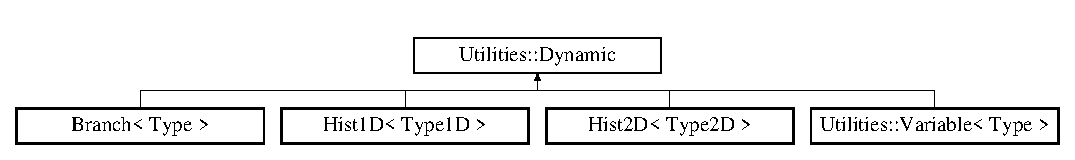
\includegraphics[height=1.696970cm]{classUtilities_1_1Dynamic}
\end{center}
\end{figure}
\doxysubsection*{Public Member Functions}
\begin{DoxyCompactItemize}
\item 
virtual \mbox{\hyperlink{classUtilities_1_1Dynamic_a4d12e083a7d3fceec2d390f47df3b992}{$\sim$\+Dynamic}} ()
\end{DoxyCompactItemize}


\doxysubsection{Detailed Description}
\char`\"{}\+Dynamic\char`\"{} object that serves as a base for templated objects 

\doxysubsection{Constructor \& Destructor Documentation}
\mbox{\Hypertarget{classUtilities_1_1Dynamic_a4d12e083a7d3fceec2d390f47df3b992}\label{classUtilities_1_1Dynamic_a4d12e083a7d3fceec2d390f47df3b992}} 
\index{Utilities::Dynamic@{Utilities::Dynamic}!````~Dynamic@{$\sim$Dynamic}}
\index{````~Dynamic@{$\sim$Dynamic}!Utilities::Dynamic@{Utilities::Dynamic}}
\doxysubsubsection{\texorpdfstring{$\sim$Dynamic()}{~Dynamic()}}
{\footnotesize\ttfamily virtual Utilities\+::\+Dynamic\+::$\sim$\+Dynamic (\begin{DoxyParamCaption}{ }\end{DoxyParamCaption})\hspace{0.3cm}{\ttfamily [virtual]}}

\mbox{\hyperlink{classUtilities_1_1Dynamic}{Dynamic}} object destructor \begin{DoxyReturn}{Returns}
none 
\end{DoxyReturn}


The documentation for this class was generated from the following file\+:\begin{DoxyCompactItemize}
\item 
/\+Users/jguiang/\+Projects/rapido/utilities.\+h\end{DoxyCompactItemize}

\hypertarget{classHEPCLI}{}\doxysection{HEPCLI Class Reference}
\label{classHEPCLI}\index{HEPCLI@{HEPCLI}}


{\ttfamily \#include $<$looper.\+h$>$}

\doxysubsection*{Public Member Functions}
\begin{DoxyCompactItemize}
\item 
\mbox{\hyperlink{classHEPCLI_a59a123c6834e44908e802b8bbeae35fc}{HEPCLI}} ()
\item 
\mbox{\hyperlink{classHEPCLI_a5812761020c8a4401f25e4469b49f6af}{HEPCLI}} (int argc, char $\ast$$\ast$argv)
\end{DoxyCompactItemize}
\doxysubsection*{Public Attributes}
\begin{DoxyCompactItemize}
\item 
bool \mbox{\hyperlink{classHEPCLI_a50592a47a23f3e33a774a747ee32bf00}{verbose}}
\item 
std\+::string \mbox{\hyperlink{classHEPCLI_ad8364ec0fda19a180ccafbdb9866790f}{input\+\_\+ttree}}
\item 
std\+::string \mbox{\hyperlink{classHEPCLI_a2c6e1c6b16b1980527bd660175e77bd8}{output\+\_\+dir}}
\item 
std\+::string \mbox{\hyperlink{classHEPCLI_a9e5f226adebb7d77fb601c93268868dd}{output\+\_\+name}}
\item 
bool \mbox{\hyperlink{classHEPCLI_a1bb98769c5df4317c50d98bff38002c1}{is\+\_\+data}}
\item 
bool \mbox{\hyperlink{classHEPCLI_ae1d563a29c5a238e0469442bad714e6e}{is\+\_\+signal}}
\item 
float \mbox{\hyperlink{classHEPCLI_a027e714e73b6fcdd0cb73eb8445bbfa4}{scale\+\_\+factor}}
\item 
TChain $\ast$ \mbox{\hyperlink{classHEPCLI_a3d4bb4a7c1f1b6d4e008ff76e43bef15}{input\+\_\+tchain}}
\end{DoxyCompactItemize}


\doxysubsection{Detailed Description}
Object for handling HEP CLI input (wraps getopt functionality) 

\doxysubsection{Constructor \& Destructor Documentation}
\mbox{\Hypertarget{classHEPCLI_a59a123c6834e44908e802b8bbeae35fc}\label{classHEPCLI_a59a123c6834e44908e802b8bbeae35fc}} 
\index{HEPCLI@{HEPCLI}!HEPCLI@{HEPCLI}}
\index{HEPCLI@{HEPCLI}!HEPCLI@{HEPCLI}}
\doxysubsubsection{\texorpdfstring{HEPCLI()}{HEPCLI()}\hspace{0.1cm}{\footnotesize\ttfamily [1/2]}}
{\footnotesize\ttfamily HEPCLI\+::\+HEPCLI (\begin{DoxyParamCaption}{ }\end{DoxyParamCaption})}

\mbox{\hyperlink{classHEPCLI}{HEPCLI}} object constructor \begin{DoxyReturn}{Returns}
none 
\end{DoxyReturn}
\mbox{\Hypertarget{classHEPCLI_a5812761020c8a4401f25e4469b49f6af}\label{classHEPCLI_a5812761020c8a4401f25e4469b49f6af}} 
\index{HEPCLI@{HEPCLI}!HEPCLI@{HEPCLI}}
\index{HEPCLI@{HEPCLI}!HEPCLI@{HEPCLI}}
\doxysubsubsection{\texorpdfstring{HEPCLI()}{HEPCLI()}\hspace{0.1cm}{\footnotesize\ttfamily [2/2]}}
{\footnotesize\ttfamily HEPCLI\+::\+HEPCLI (\begin{DoxyParamCaption}\item[{int}]{argc,  }\item[{char $\ast$$\ast$}]{argv }\end{DoxyParamCaption})}

\mbox{\hyperlink{classHEPCLI}{HEPCLI}} object overload constructor 
\begin{DoxyParams}{Parameters}
{\em argc} & argument count \\
\hline
{\em argv} & argument vector \\
\hline
\end{DoxyParams}
\begin{DoxyReturn}{Returns}
none 
\end{DoxyReturn}


\doxysubsection{Member Data Documentation}
\mbox{\Hypertarget{classHEPCLI_a3d4bb4a7c1f1b6d4e008ff76e43bef15}\label{classHEPCLI_a3d4bb4a7c1f1b6d4e008ff76e43bef15}} 
\index{HEPCLI@{HEPCLI}!input\_tchain@{input\_tchain}}
\index{input\_tchain@{input\_tchain}!HEPCLI@{HEPCLI}}
\doxysubsubsection{\texorpdfstring{input\_tchain}{input\_tchain}}
{\footnotesize\ttfamily TChain$\ast$ HEPCLI\+::input\+\_\+tchain}

ROOT TChain with input files \mbox{\Hypertarget{classHEPCLI_ad8364ec0fda19a180ccafbdb9866790f}\label{classHEPCLI_ad8364ec0fda19a180ccafbdb9866790f}} 
\index{HEPCLI@{HEPCLI}!input\_ttree@{input\_ttree}}
\index{input\_ttree@{input\_ttree}!HEPCLI@{HEPCLI}}
\doxysubsubsection{\texorpdfstring{input\_ttree}{input\_ttree}}
{\footnotesize\ttfamily std\+::string HEPCLI\+::input\+\_\+ttree}

Name of TTree in input ROOT file(s) \mbox{\Hypertarget{classHEPCLI_a1bb98769c5df4317c50d98bff38002c1}\label{classHEPCLI_a1bb98769c5df4317c50d98bff38002c1}} 
\index{HEPCLI@{HEPCLI}!is\_data@{is\_data}}
\index{is\_data@{is\_data}!HEPCLI@{HEPCLI}}
\doxysubsubsection{\texorpdfstring{is\_data}{is\_data}}
{\footnotesize\ttfamily bool HEPCLI\+::is\+\_\+data}

Data (as opposed to Monte Carlo) flag \mbox{\Hypertarget{classHEPCLI_ae1d563a29c5a238e0469442bad714e6e}\label{classHEPCLI_ae1d563a29c5a238e0469442bad714e6e}} 
\index{HEPCLI@{HEPCLI}!is\_signal@{is\_signal}}
\index{is\_signal@{is\_signal}!HEPCLI@{HEPCLI}}
\doxysubsubsection{\texorpdfstring{is\_signal}{is\_signal}}
{\footnotesize\ttfamily bool HEPCLI\+::is\+\_\+signal}

Signal (as opposed to background) flag \mbox{\Hypertarget{classHEPCLI_a2c6e1c6b16b1980527bd660175e77bd8}\label{classHEPCLI_a2c6e1c6b16b1980527bd660175e77bd8}} 
\index{HEPCLI@{HEPCLI}!output\_dir@{output\_dir}}
\index{output\_dir@{output\_dir}!HEPCLI@{HEPCLI}}
\doxysubsubsection{\texorpdfstring{output\_dir}{output\_dir}}
{\footnotesize\ttfamily std\+::string HEPCLI\+::output\+\_\+dir}

Target directory for output file(s) \mbox{\Hypertarget{classHEPCLI_a9e5f226adebb7d77fb601c93268868dd}\label{classHEPCLI_a9e5f226adebb7d77fb601c93268868dd}} 
\index{HEPCLI@{HEPCLI}!output\_name@{output\_name}}
\index{output\_name@{output\_name}!HEPCLI@{HEPCLI}}
\doxysubsubsection{\texorpdfstring{output\_name}{output\_name}}
{\footnotesize\ttfamily std\+::string HEPCLI\+::output\+\_\+name}

Short name for output file(s) \mbox{\Hypertarget{classHEPCLI_a027e714e73b6fcdd0cb73eb8445bbfa4}\label{classHEPCLI_a027e714e73b6fcdd0cb73eb8445bbfa4}} 
\index{HEPCLI@{HEPCLI}!scale\_factor@{scale\_factor}}
\index{scale\_factor@{scale\_factor}!HEPCLI@{HEPCLI}}
\doxysubsubsection{\texorpdfstring{scale\_factor}{scale\_factor}}
{\footnotesize\ttfamily float HEPCLI\+::scale\+\_\+factor}

Global event weight \mbox{\Hypertarget{classHEPCLI_a50592a47a23f3e33a774a747ee32bf00}\label{classHEPCLI_a50592a47a23f3e33a774a747ee32bf00}} 
\index{HEPCLI@{HEPCLI}!verbose@{verbose}}
\index{verbose@{verbose}!HEPCLI@{HEPCLI}}
\doxysubsubsection{\texorpdfstring{verbose}{verbose}}
{\footnotesize\ttfamily bool HEPCLI\+::verbose}

Verbosity flag 

The documentation for this class was generated from the following file\+:\begin{DoxyCompactItemize}
\item 
/github/workspace/rapido/src/looper.\+h\end{DoxyCompactItemize}

\hypertarget{classHist1D}{}\doxysection{Hist1D\texorpdfstring{$<$}{<} Type1D \texorpdfstring{$>$}{>} Class Template Reference}
\label{classHist1D}\index{Hist1D$<$ Type1D $>$@{Hist1D$<$ Type1D $>$}}


{\ttfamily \#include $<$histflow.\+h$>$}

Inheritance diagram for Hist1D\texorpdfstring{$<$}{<} Type1D \texorpdfstring{$>$}{>}\+:\begin{figure}[H]
\begin{center}
\leavevmode
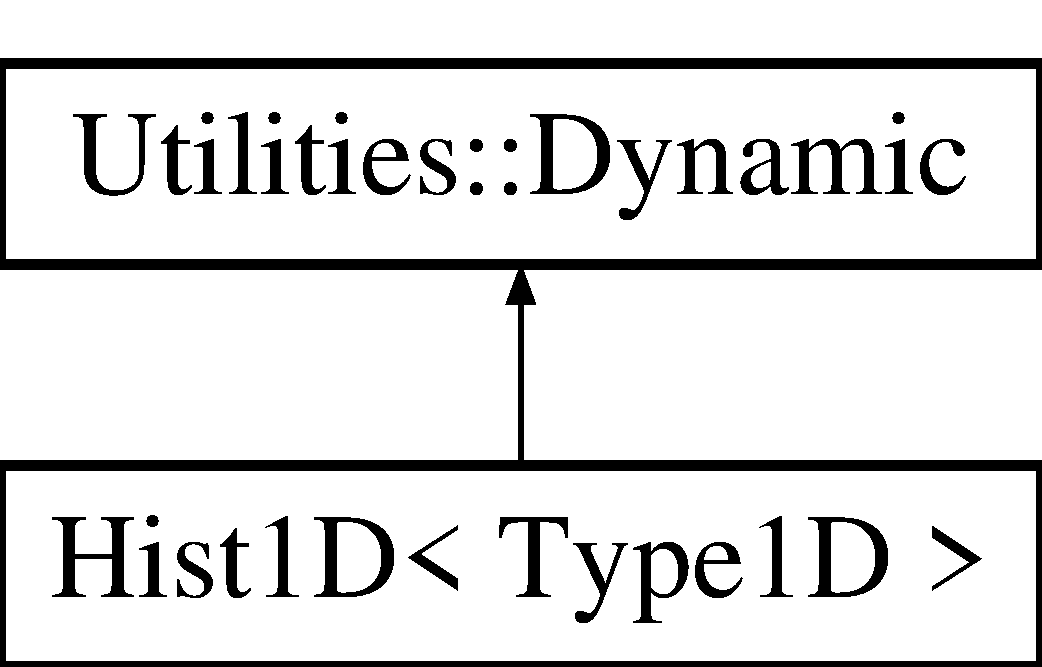
\includegraphics[height=2.000000cm]{classHist1D}
\end{center}
\end{figure}
\doxysubsection*{Public Member Functions}
\begin{DoxyCompactItemize}
\item 
\mbox{\hyperlink{classHist1D_a76378975401f2dcd3635244ca8614664}{Hist1D}} (Type1D $\ast$new\+\_\+hist, Filler1D new\+\_\+filler)
\item 
\mbox{\hyperlink{classHist1D_a26a713a3b0f55a885fd6f110407990ee}{$\sim$\+Hist1D}} ()
\item 
void \mbox{\hyperlink{classHist1D_af9ae5dd7a2aca46be456dde196db8fba}{fill}} (float weight=1.\+0)
\item 
void \mbox{\hyperlink{classHist1D_ae45c2073b4c8f25a10ac534012feb22b}{write}} ()
\item 
\mbox{\hyperlink{classHist1D}{Hist1D}}$<$ Type1D $>$ $\ast$ \mbox{\hyperlink{classHist1D_a68aaeba84e870ae5a117fe49c21f3a7c}{clone}} ()
\end{DoxyCompactItemize}
\doxysubsection*{Public Attributes}
\begin{DoxyCompactItemize}
\item 
TString \mbox{\hyperlink{classHist1D_a28f350f4fd9e13199ef560ea6820d65c}{name}}
\end{DoxyCompactItemize}


\doxysubsection{Detailed Description}
\subsubsection*{template$<$typename Type1D$>$\newline
class Hist1\+D$<$ Type1\+D $>$}
\char`\"{}\+Dynamic\char`\"{} 1D ROOT histogram object 
\begin{DoxyTemplParams}{Template Parameters}
{\em Type1D} & type of 1D ROOT histogram (e.\+g. TH1F) \\
\hline
\end{DoxyTemplParams}


\doxysubsection{Constructor \& Destructor Documentation}
\mbox{\Hypertarget{classHist1D_a76378975401f2dcd3635244ca8614664}\label{classHist1D_a76378975401f2dcd3635244ca8614664}} 
\index{Hist1D$<$ Type1D $>$@{Hist1D$<$ Type1D $>$}!Hist1D@{Hist1D}}
\index{Hist1D@{Hist1D}!Hist1D$<$ Type1D $>$@{Hist1D$<$ Type1D $>$}}
\doxysubsubsection{\texorpdfstring{Hist1D()}{Hist1D()}}
{\footnotesize\ttfamily template$<$typename Type1D $>$ \\
\mbox{\hyperlink{classHist1D}{Hist1D}}$<$ Type1D $>$\mbox{\hyperlink{classHist1D}{\+::\+Hist1D}} (\begin{DoxyParamCaption}\item[{Type1D $\ast$}]{new\+\_\+hist,  }\item[{Filler1D}]{new\+\_\+filler }\end{DoxyParamCaption})}

1D Histogram constructor 
\begin{DoxyParams}{Parameters}
{\em new\+\_\+hist} & pointer to a 1D ROOT histogram \\
\hline
{\em new\+\_\+filler} & lambda function that computes the value used to fill the histogram \\
\hline
\end{DoxyParams}
\begin{DoxyReturn}{Returns}
none 
\end{DoxyReturn}
\mbox{\Hypertarget{classHist1D_a26a713a3b0f55a885fd6f110407990ee}\label{classHist1D_a26a713a3b0f55a885fd6f110407990ee}} 
\index{Hist1D$<$ Type1D $>$@{Hist1D$<$ Type1D $>$}!````~Hist1D@{$\sim$Hist1D}}
\index{````~Hist1D@{$\sim$Hist1D}!Hist1D$<$ Type1D $>$@{Hist1D$<$ Type1D $>$}}
\doxysubsubsection{\texorpdfstring{$\sim$Hist1D()}{~Hist1D()}}
{\footnotesize\ttfamily template$<$typename Type1D $>$ \\
\mbox{\hyperlink{classHist1D}{Hist1D}}$<$ Type1D $>$\+::$\sim$\mbox{\hyperlink{classHist1D}{Hist1D}} (\begin{DoxyParamCaption}{ }\end{DoxyParamCaption})}

1D Histogram destructor \begin{DoxyReturn}{Returns}
none 
\end{DoxyReturn}


\doxysubsection{Member Function Documentation}
\mbox{\Hypertarget{classHist1D_a68aaeba84e870ae5a117fe49c21f3a7c}\label{classHist1D_a68aaeba84e870ae5a117fe49c21f3a7c}} 
\index{Hist1D$<$ Type1D $>$@{Hist1D$<$ Type1D $>$}!clone@{clone}}
\index{clone@{clone}!Hist1D$<$ Type1D $>$@{Hist1D$<$ Type1D $>$}}
\doxysubsubsection{\texorpdfstring{clone()}{clone()}}
{\footnotesize\ttfamily template$<$typename Type1D $>$ \\
\mbox{\hyperlink{classHist1D}{Hist1D}}$<$ Type1D $>$ $\ast$ \mbox{\hyperlink{classHist1D}{Hist1D}}$<$ Type1D $>$\+::clone (\begin{DoxyParamCaption}{ }\end{DoxyParamCaption})}

Clone this \char`\"{}dynamic\char`\"{} histogram object \begin{DoxyReturn}{Returns}
none 
\end{DoxyReturn}
\mbox{\Hypertarget{classHist1D_af9ae5dd7a2aca46be456dde196db8fba}\label{classHist1D_af9ae5dd7a2aca46be456dde196db8fba}} 
\index{Hist1D$<$ Type1D $>$@{Hist1D$<$ Type1D $>$}!fill@{fill}}
\index{fill@{fill}!Hist1D$<$ Type1D $>$@{Hist1D$<$ Type1D $>$}}
\doxysubsubsection{\texorpdfstring{fill()}{fill()}}
{\footnotesize\ttfamily template$<$typename Type1D $>$ \\
void \mbox{\hyperlink{classHist1D}{Hist1D}}$<$ Type1D $>$\+::fill (\begin{DoxyParamCaption}\item[{float}]{weight = {\ttfamily 1.0} }\end{DoxyParamCaption})}

Call filler to fill histogram with an optional weight 
\begin{DoxyParams}{Parameters}
{\em weight} & float to weigh new histogram entry (optional) \\
\hline
\end{DoxyParams}
\begin{DoxyReturn}{Returns}
none 
\end{DoxyReturn}
\mbox{\Hypertarget{classHist1D_ae45c2073b4c8f25a10ac534012feb22b}\label{classHist1D_ae45c2073b4c8f25a10ac534012feb22b}} 
\index{Hist1D$<$ Type1D $>$@{Hist1D$<$ Type1D $>$}!write@{write}}
\index{write@{write}!Hist1D$<$ Type1D $>$@{Hist1D$<$ Type1D $>$}}
\doxysubsubsection{\texorpdfstring{write()}{write()}}
{\footnotesize\ttfamily template$<$typename Type1D $>$ \\
void \mbox{\hyperlink{classHist1D}{Hist1D}}$<$ Type1D $>$\+::write (\begin{DoxyParamCaption}{ }\end{DoxyParamCaption})}

Write ROOT histogram to currently opened TFile \begin{DoxyReturn}{Returns}
none 
\end{DoxyReturn}


\doxysubsection{Member Data Documentation}
\mbox{\Hypertarget{classHist1D_a28f350f4fd9e13199ef560ea6820d65c}\label{classHist1D_a28f350f4fd9e13199ef560ea6820d65c}} 
\index{Hist1D$<$ Type1D $>$@{Hist1D$<$ Type1D $>$}!name@{name}}
\index{name@{name}!Hist1D$<$ Type1D $>$@{Hist1D$<$ Type1D $>$}}
\doxysubsubsection{\texorpdfstring{name}{name}}
{\footnotesize\ttfamily template$<$typename Type1D $>$ \\
TString \mbox{\hyperlink{classHist1D}{Hist1D}}$<$ Type1D $>$\+::name}

Name of histogram 

The documentation for this class was generated from the following file\+:\begin{DoxyCompactItemize}
\item 
/\+Users/jguiang/\+Projects/rapido/src/histflow.\+h\end{DoxyCompactItemize}

\hypertarget{classHist2D}{}\doxysection{Hist2D\texorpdfstring{$<$}{<} Type2D \texorpdfstring{$>$}{>} Class Template Reference}
\label{classHist2D}\index{Hist2D$<$ Type2D $>$@{Hist2D$<$ Type2D $>$}}


{\ttfamily \#include $<$histflow.\+h$>$}

Inheritance diagram for Hist2D\texorpdfstring{$<$}{<} Type2D \texorpdfstring{$>$}{>}\+:\begin{figure}[H]
\begin{center}
\leavevmode
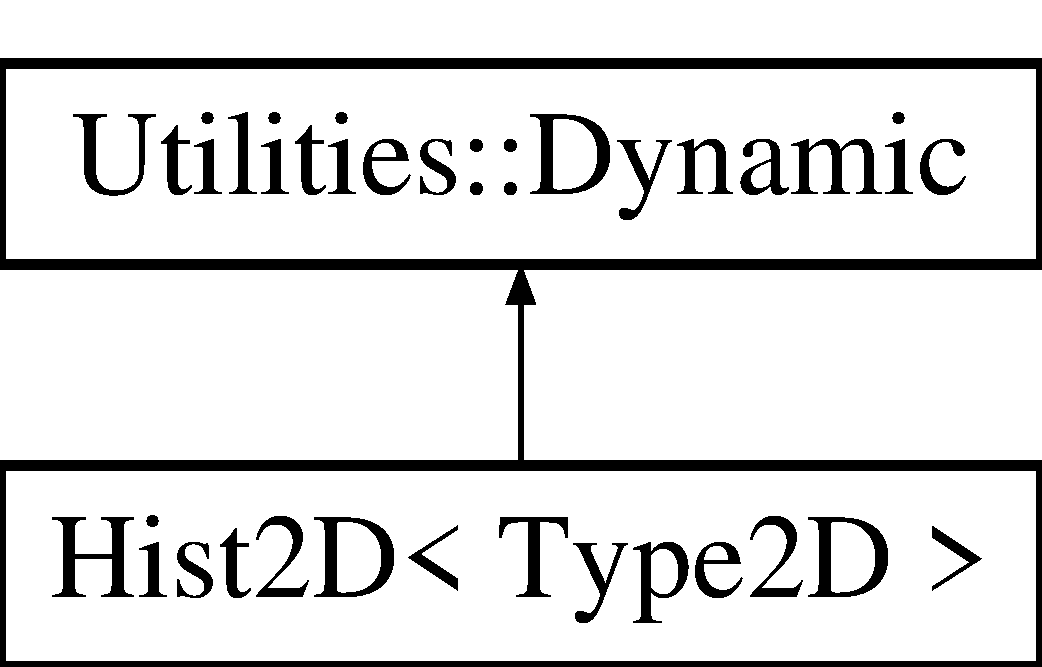
\includegraphics[height=2.000000cm]{classHist2D}
\end{center}
\end{figure}
\doxysubsection*{Public Member Functions}
\begin{DoxyCompactItemize}
\item 
\mbox{\hyperlink{classHist2D_a85a6f8b45d8752b1c50a3ea1c1436860}{Hist2D}} (Type2D $\ast$new\+\_\+hist, Filler2D new\+\_\+filler)
\item 
\mbox{\hyperlink{classHist2D_ae100dde5b1716fc0033102f3db6dece1}{$\sim$\+Hist2D}} ()
\item 
void \mbox{\hyperlink{classHist2D_a851f1d896300cb1962e5ac87a176cb08}{fill}} (float weight=1.\+0)
\item 
void \mbox{\hyperlink{classHist2D_aea99923e54c6b1af26c2b399cf648231}{write}} ()
\item 
\mbox{\hyperlink{classHist2D}{Hist2D}} $\ast$ \mbox{\hyperlink{classHist2D_aba7e37236e77fcefb39c839c39261c73}{clone}} ()
\end{DoxyCompactItemize}
\doxysubsection*{Public Attributes}
\begin{DoxyCompactItemize}
\item 
TString \mbox{\hyperlink{classHist2D_ac84b99dc72ad3d9f85a46f7620ce1740}{name}}
\end{DoxyCompactItemize}


\doxysubsection{Detailed Description}
\subsubsection*{template$<$typename Type2D$>$\newline
class Hist2\+D$<$ Type2\+D $>$}
\char`\"{}\+Dynamic\char`\"{} 2D ROOT histogram object 
\begin{DoxyTemplParams}{Template Parameters}
{\em Type2D} & type of 2D ROOT histogram (e.\+g. TH2F) \\
\hline
\end{DoxyTemplParams}


\doxysubsection{Constructor \& Destructor Documentation}
\mbox{\Hypertarget{classHist2D_a85a6f8b45d8752b1c50a3ea1c1436860}\label{classHist2D_a85a6f8b45d8752b1c50a3ea1c1436860}} 
\index{Hist2D$<$ Type2D $>$@{Hist2D$<$ Type2D $>$}!Hist2D@{Hist2D}}
\index{Hist2D@{Hist2D}!Hist2D$<$ Type2D $>$@{Hist2D$<$ Type2D $>$}}
\doxysubsubsection{\texorpdfstring{Hist2D()}{Hist2D()}}
{\footnotesize\ttfamily template$<$typename Type2D $>$ \\
\mbox{\hyperlink{classHist2D}{Hist2D}}$<$ Type2D $>$\mbox{\hyperlink{classHist2D}{\+::\+Hist2D}} (\begin{DoxyParamCaption}\item[{Type2D $\ast$}]{new\+\_\+hist,  }\item[{Filler2D}]{new\+\_\+filler }\end{DoxyParamCaption})}

2D Histogram constructor 
\begin{DoxyParams}{Parameters}
{\em new\+\_\+hist} & pointer to a 2D ROOT histogram \\
\hline
{\em new\+\_\+filler} & lambda function that computes the value used to fill the histogram \\
\hline
\end{DoxyParams}
\begin{DoxyReturn}{Returns}
none 
\end{DoxyReturn}
\mbox{\Hypertarget{classHist2D_ae100dde5b1716fc0033102f3db6dece1}\label{classHist2D_ae100dde5b1716fc0033102f3db6dece1}} 
\index{Hist2D$<$ Type2D $>$@{Hist2D$<$ Type2D $>$}!````~Hist2D@{$\sim$Hist2D}}
\index{````~Hist2D@{$\sim$Hist2D}!Hist2D$<$ Type2D $>$@{Hist2D$<$ Type2D $>$}}
\doxysubsubsection{\texorpdfstring{$\sim$Hist2D()}{~Hist2D()}}
{\footnotesize\ttfamily template$<$typename Type2D $>$ \\
\mbox{\hyperlink{classHist2D}{Hist2D}}$<$ Type2D $>$\+::$\sim$\mbox{\hyperlink{classHist2D}{Hist2D}} (\begin{DoxyParamCaption}{ }\end{DoxyParamCaption})}

2D Histogram destructor \begin{DoxyReturn}{Returns}
none 
\end{DoxyReturn}


\doxysubsection{Member Function Documentation}
\mbox{\Hypertarget{classHist2D_aba7e37236e77fcefb39c839c39261c73}\label{classHist2D_aba7e37236e77fcefb39c839c39261c73}} 
\index{Hist2D$<$ Type2D $>$@{Hist2D$<$ Type2D $>$}!clone@{clone}}
\index{clone@{clone}!Hist2D$<$ Type2D $>$@{Hist2D$<$ Type2D $>$}}
\doxysubsubsection{\texorpdfstring{clone()}{clone()}}
{\footnotesize\ttfamily template$<$typename Type2D $>$ \\
\mbox{\hyperlink{classHist2D}{Hist2D}} $\ast$ \mbox{\hyperlink{classHist2D}{Hist2D}}$<$ Type2D $>$\+::clone (\begin{DoxyParamCaption}{ }\end{DoxyParamCaption})}

Clone this \char`\"{}dynamic\char`\"{} histogram object \begin{DoxyReturn}{Returns}
none 
\end{DoxyReturn}
\mbox{\Hypertarget{classHist2D_a851f1d896300cb1962e5ac87a176cb08}\label{classHist2D_a851f1d896300cb1962e5ac87a176cb08}} 
\index{Hist2D$<$ Type2D $>$@{Hist2D$<$ Type2D $>$}!fill@{fill}}
\index{fill@{fill}!Hist2D$<$ Type2D $>$@{Hist2D$<$ Type2D $>$}}
\doxysubsubsection{\texorpdfstring{fill()}{fill()}}
{\footnotesize\ttfamily template$<$typename Type2D $>$ \\
void \mbox{\hyperlink{classHist2D}{Hist2D}}$<$ Type2D $>$\+::fill (\begin{DoxyParamCaption}\item[{float}]{weight = {\ttfamily 1.0} }\end{DoxyParamCaption})}

Call filler to fill histogram with an optional weight 
\begin{DoxyParams}{Parameters}
{\em weight} & float to weigh new histogram entry (optional) \\
\hline
\end{DoxyParams}
\begin{DoxyReturn}{Returns}
none 
\end{DoxyReturn}
\mbox{\Hypertarget{classHist2D_aea99923e54c6b1af26c2b399cf648231}\label{classHist2D_aea99923e54c6b1af26c2b399cf648231}} 
\index{Hist2D$<$ Type2D $>$@{Hist2D$<$ Type2D $>$}!write@{write}}
\index{write@{write}!Hist2D$<$ Type2D $>$@{Hist2D$<$ Type2D $>$}}
\doxysubsubsection{\texorpdfstring{write()}{write()}}
{\footnotesize\ttfamily template$<$typename Type2D $>$ \\
void \mbox{\hyperlink{classHist2D}{Hist2D}}$<$ Type2D $>$\+::write (\begin{DoxyParamCaption}{ }\end{DoxyParamCaption})}

Write ROOT histogram to currently opened TFile \begin{DoxyReturn}{Returns}
none 
\end{DoxyReturn}


\doxysubsection{Member Data Documentation}
\mbox{\Hypertarget{classHist2D_ac84b99dc72ad3d9f85a46f7620ce1740}\label{classHist2D_ac84b99dc72ad3d9f85a46f7620ce1740}} 
\index{Hist2D$<$ Type2D $>$@{Hist2D$<$ Type2D $>$}!name@{name}}
\index{name@{name}!Hist2D$<$ Type2D $>$@{Hist2D$<$ Type2D $>$}}
\doxysubsubsection{\texorpdfstring{name}{name}}
{\footnotesize\ttfamily template$<$typename Type2D $>$ \\
TString \mbox{\hyperlink{classHist2D}{Hist2D}}$<$ Type2D $>$\+::name}

Name of histogram 

The documentation for this class was generated from the following file\+:\begin{DoxyCompactItemize}
\item 
/\+Users/jguiang/\+Projects/rapido/histflow.\+h\end{DoxyCompactItemize}

\hypertarget{classHistflow}{}\doxysection{Histflow Class Reference}
\label{classHistflow}\index{Histflow@{Histflow}}


{\ttfamily \#include $<$histflow.\+h$>$}

Inheritance diagram for Histflow\+:\begin{figure}[H]
\begin{center}
\leavevmode
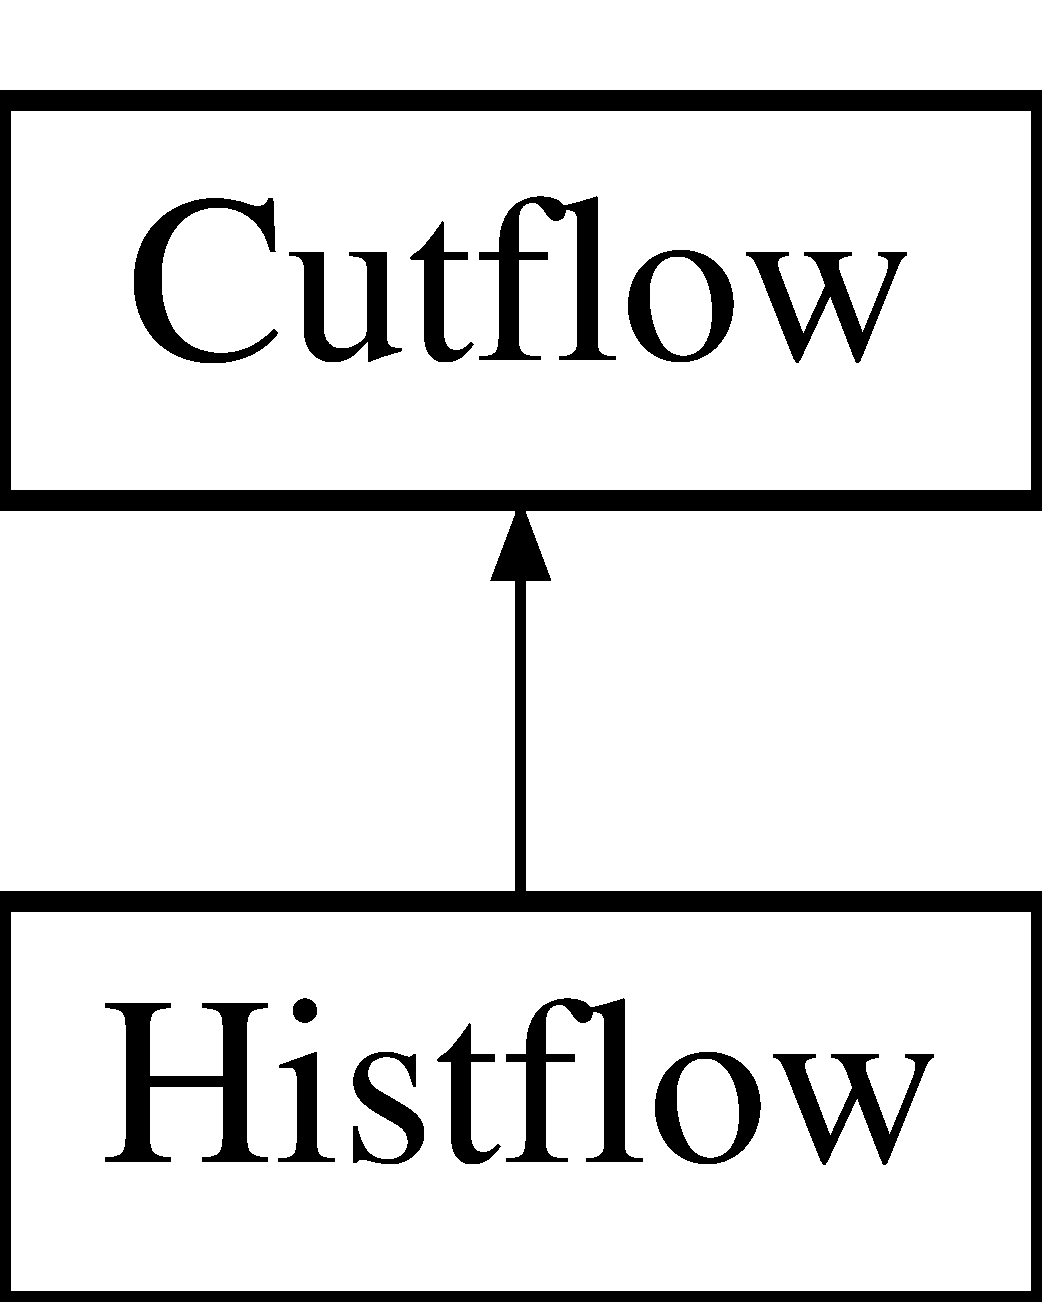
\includegraphics[height=2.000000cm]{classHistflow}
\end{center}
\end{figure}
\doxysubsection*{Public Member Functions}
\begin{DoxyCompactItemize}
\item 
\mbox{\hyperlink{classHistflow_ae4c76353f6d545eca787fc0abf1a433e}{Histflow}} ()
\item 
\mbox{\hyperlink{classHistflow_aa1adf4cd5e253c51f4e9febf97e11da1}{$\sim$\+Histflow}} ()
\item 
{\footnotesize template$<$typename Type1D $>$ }\\void \mbox{\hyperlink{classHistflow_a0fc41c86984acdd1b2a271be83ecf69d}{book\+Hist1D}} (std\+::string target\+\_\+cut\+\_\+name, \mbox{\hyperlink{classHist1D}{Hist1D}}$<$ Type1D $>$ $\ast$hist)
\item 
{\footnotesize template$<$typename Type2D $>$ }\\void \mbox{\hyperlink{classHistflow_a16858deb3566f6b64c4ac21c309d0a2c}{book\+Hist2D}} (std\+::string target\+\_\+cut\+\_\+name, \mbox{\hyperlink{classHist2D}{Hist2D}}$<$ Type2D $>$ $\ast$hist)
\item 
{\footnotesize template$<$typename Type1D $>$ }\\void \mbox{\hyperlink{classHistflow_a07a698624a6376ebdcef8ef9b025ef33}{book\+Hist1D}} (std\+::string target\+\_\+cut\+\_\+name, Type1D $\ast$hist, Filler1D filler)
\item 
{\footnotesize template$<$typename Type2D $>$ }\\void \mbox{\hyperlink{classHistflow_a425698092efa7ec2389b9fb83d26dc84}{book\+Hist2D}} (std\+::string target\+\_\+cut\+\_\+name, Type2D $\ast$hist, Filler2D filler)
\item 
void \mbox{\hyperlink{classHistflow_a06a2e1683cdc7ac2731b4608abe15eb7}{write\+Hists}} (TFile $\ast$tfile)
\item 
\mbox{\hyperlink{classCut}{Cut}} $\ast$ \mbox{\hyperlink{classHistflow_a675b897276d33e146d1c2707023f1edd}{run}} () override
\end{DoxyCompactItemize}
\doxysubsection*{Protected Member Functions}
\begin{DoxyCompactItemize}
\item 
\mbox{\hyperlink{classCut}{Cut}} $\ast$ \mbox{\hyperlink{classHistflow_a5f82e40b32a417161fbcfa0daaf1f8e0}{recursive\+Evaluate}} (\mbox{\hyperlink{classCut}{Cut}} $\ast$cut, float weight=1.\+0)
\end{DoxyCompactItemize}
\doxysubsection*{Protected Attributes}
\begin{DoxyCompactItemize}
\item 
std\+::map$<$ std\+::string, std\+::vector$<$ std\+::function$<$ void(float)$>$ $>$ $>$ \mbox{\hyperlink{classHistflow_a8440049297c1fc5d0c0f71602a940850}{fill\+\_\+schedule}}
\item 
std\+::map$<$ TString, std\+::function$<$ void()$>$ $>$ \mbox{\hyperlink{classHistflow_ab0e1c8893b1afe8b77c886f6c7c043f4}{hist\+\_\+writers}}
\end{DoxyCompactItemize}
\doxysubsection*{Additional Inherited Members}


\doxysubsection{Detailed Description}
Modified \mbox{\hyperlink{classCutflow}{Cutflow}} object that fills booked histograms after passing a given set of cuts 

\doxysubsection{Constructor \& Destructor Documentation}
\mbox{\Hypertarget{classHistflow_ae4c76353f6d545eca787fc0abf1a433e}\label{classHistflow_ae4c76353f6d545eca787fc0abf1a433e}} 
\index{Histflow@{Histflow}!Histflow@{Histflow}}
\index{Histflow@{Histflow}!Histflow@{Histflow}}
\doxysubsubsection{\texorpdfstring{Histflow()}{Histflow()}}
{\footnotesize\ttfamily Histflow\+::\+Histflow (\begin{DoxyParamCaption}{ }\end{DoxyParamCaption})}

\mbox{\hyperlink{classHistflow}{Histflow}} constructor \begin{DoxyReturn}{Returns}
none 
\end{DoxyReturn}
\mbox{\Hypertarget{classHistflow_aa1adf4cd5e253c51f4e9febf97e11da1}\label{classHistflow_aa1adf4cd5e253c51f4e9febf97e11da1}} 
\index{Histflow@{Histflow}!````~Histflow@{$\sim$Histflow}}
\index{````~Histflow@{$\sim$Histflow}!Histflow@{Histflow}}
\doxysubsubsection{\texorpdfstring{$\sim$Histflow()}{~Histflow()}}
{\footnotesize\ttfamily Histflow\+::$\sim$\+Histflow (\begin{DoxyParamCaption}{ }\end{DoxyParamCaption})}

\mbox{\hyperlink{classHistflow}{Histflow}} destructor \begin{DoxyReturn}{Returns}
none 
\end{DoxyReturn}


\doxysubsection{Member Function Documentation}
\mbox{\Hypertarget{classHistflow_a0fc41c86984acdd1b2a271be83ecf69d}\label{classHistflow_a0fc41c86984acdd1b2a271be83ecf69d}} 
\index{Histflow@{Histflow}!bookHist1D@{bookHist1D}}
\index{bookHist1D@{bookHist1D}!Histflow@{Histflow}}
\doxysubsubsection{\texorpdfstring{bookHist1D()}{bookHist1D()}\hspace{0.1cm}{\footnotesize\ttfamily [1/2]}}
{\footnotesize\ttfamily template$<$typename Type1D $>$ \\
void Histflow\+::book\+Hist1D (\begin{DoxyParamCaption}\item[{std\+::string}]{target\+\_\+cut\+\_\+name,  }\item[{\mbox{\hyperlink{classHist1D}{Hist1D}}$<$ Type1D $>$ $\ast$}]{hist }\end{DoxyParamCaption})}

Schedule a \char`\"{}dynamic\char`\"{} 1D histogram object for a given cut 
\begin{DoxyParams}{Parameters}
{\em target\+\_\+cut\+\_\+name} & target node name \\
\hline
{\em hist} & pointer to \char`\"{}dynamic\char`\"{} 1D histogram object to schedule \\
\hline
\end{DoxyParams}
\begin{DoxyReturn}{Returns}
none 
\end{DoxyReturn}
\mbox{\Hypertarget{classHistflow_a07a698624a6376ebdcef8ef9b025ef33}\label{classHistflow_a07a698624a6376ebdcef8ef9b025ef33}} 
\index{Histflow@{Histflow}!bookHist1D@{bookHist1D}}
\index{bookHist1D@{bookHist1D}!Histflow@{Histflow}}
\doxysubsubsection{\texorpdfstring{bookHist1D()}{bookHist1D()}\hspace{0.1cm}{\footnotesize\ttfamily [2/2]}}
{\footnotesize\ttfamily template$<$typename Type1D $>$ \\
void Histflow\+::book\+Hist1D (\begin{DoxyParamCaption}\item[{std\+::string}]{target\+\_\+cut\+\_\+name,  }\item[{Type1D $\ast$}]{hist,  }\item[{Filler1D}]{filler }\end{DoxyParamCaption})}

Schedule a 1D ROOT histogram for a given cut 
\begin{DoxyParams}{Parameters}
{\em target\+\_\+cut\+\_\+name} & target node name \\
\hline
{\em hist} & pointer to 1D ROOT histogram to schedule \\
\hline
{\em filler} & lambda function that computes the value used to fill the histogram \\
\hline
\end{DoxyParams}
\begin{DoxyReturn}{Returns}
none 
\end{DoxyReturn}
\mbox{\Hypertarget{classHistflow_a16858deb3566f6b64c4ac21c309d0a2c}\label{classHistflow_a16858deb3566f6b64c4ac21c309d0a2c}} 
\index{Histflow@{Histflow}!bookHist2D@{bookHist2D}}
\index{bookHist2D@{bookHist2D}!Histflow@{Histflow}}
\doxysubsubsection{\texorpdfstring{bookHist2D()}{bookHist2D()}\hspace{0.1cm}{\footnotesize\ttfamily [1/2]}}
{\footnotesize\ttfamily template$<$typename Type2D $>$ \\
void Histflow\+::book\+Hist2D (\begin{DoxyParamCaption}\item[{std\+::string}]{target\+\_\+cut\+\_\+name,  }\item[{\mbox{\hyperlink{classHist2D}{Hist2D}}$<$ Type2D $>$ $\ast$}]{hist }\end{DoxyParamCaption})}

Schedule a \char`\"{}dynamic\char`\"{} 2D histogram object for a given cut 
\begin{DoxyParams}{Parameters}
{\em target\+\_\+cut\+\_\+name} & target node name \\
\hline
{\em hist} & pointer to \char`\"{}dynamic\char`\"{} 2D histogram object to schedule \\
\hline
\end{DoxyParams}
\begin{DoxyReturn}{Returns}
none 
\end{DoxyReturn}
\mbox{\Hypertarget{classHistflow_a425698092efa7ec2389b9fb83d26dc84}\label{classHistflow_a425698092efa7ec2389b9fb83d26dc84}} 
\index{Histflow@{Histflow}!bookHist2D@{bookHist2D}}
\index{bookHist2D@{bookHist2D}!Histflow@{Histflow}}
\doxysubsubsection{\texorpdfstring{bookHist2D()}{bookHist2D()}\hspace{0.1cm}{\footnotesize\ttfamily [2/2]}}
{\footnotesize\ttfamily template$<$typename Type2D $>$ \\
void Histflow\+::book\+Hist2D (\begin{DoxyParamCaption}\item[{std\+::string}]{target\+\_\+cut\+\_\+name,  }\item[{Type2D $\ast$}]{hist,  }\item[{Filler2D}]{filler }\end{DoxyParamCaption})}

Schedule a 2D ROOT histogram for a given cut 
\begin{DoxyParams}{Parameters}
{\em target\+\_\+cut\+\_\+name} & target node name \\
\hline
{\em hist} & pointer to 2D ROOT histogram to schedule \\
\hline
{\em filler} & lambda function that computes the value used to fill the histogram \\
\hline
\end{DoxyParams}
\begin{DoxyReturn}{Returns}
none 
\end{DoxyReturn}
\mbox{\Hypertarget{classHistflow_a5f82e40b32a417161fbcfa0daaf1f8e0}\label{classHistflow_a5f82e40b32a417161fbcfa0daaf1f8e0}} 
\index{Histflow@{Histflow}!recursiveEvaluate@{recursiveEvaluate}}
\index{recursiveEvaluate@{recursiveEvaluate}!Histflow@{Histflow}}
\doxysubsubsection{\texorpdfstring{recursiveEvaluate()}{recursiveEvaluate()}}
{\footnotesize\ttfamily \mbox{\hyperlink{classCut}{Cut}} $\ast$ Histflow\+::recursive\+Evaluate (\begin{DoxyParamCaption}\item[{\mbox{\hyperlink{classCut}{Cut}} $\ast$}]{cut,  }\item[{float}]{weight = {\ttfamily 1.0} }\end{DoxyParamCaption})\hspace{0.3cm}{\ttfamily [protected]}}

(PROTECTED) Additional definition that recursively evaluates cuts in cutflow and fills scheduled histograms when appropriate cuts are passed 
\begin{DoxyParams}{Parameters}
{\em cut} & pointer to current cut \\
\hline
{\em weight} & current event weight (optional) \\
\hline
\end{DoxyParams}
\begin{DoxyReturn}{Returns}
none 
\end{DoxyReturn}
\mbox{\Hypertarget{classHistflow_a675b897276d33e146d1c2707023f1edd}\label{classHistflow_a675b897276d33e146d1c2707023f1edd}} 
\index{Histflow@{Histflow}!run@{run}}
\index{run@{run}!Histflow@{Histflow}}
\doxysubsubsection{\texorpdfstring{run()}{run()}}
{\footnotesize\ttfamily \mbox{\hyperlink{classCut}{Cut}} $\ast$ Histflow\+::run (\begin{DoxyParamCaption}{ }\end{DoxyParamCaption})\hspace{0.3cm}{\ttfamily [override]}, {\ttfamily [virtual]}}

Overriding definition that runs cutflow with \mbox{\hyperlink{classHistflow_a5f82e40b32a417161fbcfa0daaf1f8e0}{Histflow\+::recursive\+Evaluate}} \begin{DoxyReturn}{Returns}
pointer to terminal cut (final leaf of tree reached) 
\end{DoxyReturn}


Reimplemented from \mbox{\hyperlink{classCutflow_a8fc98b9c006b80db96576c8bdcf6a0a8}{Cutflow}}.

\mbox{\Hypertarget{classHistflow_a06a2e1683cdc7ac2731b4608abe15eb7}\label{classHistflow_a06a2e1683cdc7ac2731b4608abe15eb7}} 
\index{Histflow@{Histflow}!writeHists@{writeHists}}
\index{writeHists@{writeHists}!Histflow@{Histflow}}
\doxysubsubsection{\texorpdfstring{writeHists()}{writeHists()}}
{\footnotesize\ttfamily void Histflow\+::write\+Hists (\begin{DoxyParamCaption}\item[{TFile $\ast$}]{tfile }\end{DoxyParamCaption})}

Write all histograms to a given TFile 
\begin{DoxyParams}{Parameters}
{\em tfile} & pointer to ROOT TFile to write histograms to \\
\hline
\end{DoxyParams}
\begin{DoxyReturn}{Returns}
none 
\end{DoxyReturn}


\doxysubsection{Member Data Documentation}
\mbox{\Hypertarget{classHistflow_a8440049297c1fc5d0c0f71602a940850}\label{classHistflow_a8440049297c1fc5d0c0f71602a940850}} 
\index{Histflow@{Histflow}!fill\_schedule@{fill\_schedule}}
\index{fill\_schedule@{fill\_schedule}!Histflow@{Histflow}}
\doxysubsubsection{\texorpdfstring{fill\_schedule}{fill\_schedule}}
{\footnotesize\ttfamily std\+::map$<$std\+::string, std\+::vector$<$std\+::function$<$void(float)$>$ $>$ $>$ Histflow\+::fill\+\_\+schedule\hspace{0.3cm}{\ttfamily [protected]}}

\char`\"{}\+Schedule\char`\"{} dictating when to fill certain histograms \mbox{\Hypertarget{classHistflow_ab0e1c8893b1afe8b77c886f6c7c043f4}\label{classHistflow_ab0e1c8893b1afe8b77c886f6c7c043f4}} 
\index{Histflow@{Histflow}!hist\_writers@{hist\_writers}}
\index{hist\_writers@{hist\_writers}!Histflow@{Histflow}}
\doxysubsubsection{\texorpdfstring{hist\_writers}{hist\_writers}}
{\footnotesize\ttfamily std\+::map$<$TString, std\+::function$<$void()$>$ $>$ Histflow\+::hist\+\_\+writers\hspace{0.3cm}{\ttfamily [protected]}}

Collection of functions that write histograms to opened TFile 

The documentation for this class was generated from the following file\+:\begin{DoxyCompactItemize}
\item 
/github/workspace/rapido/src/histflow.\+h\end{DoxyCompactItemize}

\hypertarget{classLooper}{}\doxysection{Looper Class Reference}
\label{classLooper}\index{Looper@{Looper}}


{\ttfamily \#include $<$looper.\+h$>$}

\doxysubsection*{Public Member Functions}
\begin{DoxyCompactItemize}
\item 
\mbox{\hyperlink{classLooper_a916868e8a7a8bf73274a82bf47df22f4}{Looper}} (TChain $\ast$new\+\_\+tchain)
\item 
virtual \mbox{\hyperlink{classLooper_a23ff9511f1d99ca1f3753e59a1b3a22b}{$\sim$\+Looper}} ()
\item 
void \mbox{\hyperlink{classLooper_a8b259a7ad0c2aa45ae49d1ec08d37af0}{run}} (std\+::function$<$ void(TTree $\ast$ttree)$>$ init, std\+::function$<$ void(int entry)$>$ eval)
\end{DoxyCompactItemize}
\doxysubsection*{Public Attributes}
\begin{DoxyCompactItemize}
\item 
TChain $\ast$ \mbox{\hyperlink{classLooper_ae804a8c01aea03c415a0277099b7a2a0}{tchain}}
\item 
TString \mbox{\hyperlink{classLooper_aa42e5d8d2e16cf7768ea5d582a17868c}{ttree\+\_\+name}}
\item 
unsigned int \mbox{\hyperlink{classLooper_ab368e58278fc91c4814e579cb9080d4f}{current\+\_\+entry}}
\item 
unsigned int \mbox{\hyperlink{classLooper_abbf626538aced372130172ac86958265}{n\+\_\+events\+\_\+processed}}
\item 
unsigned int \mbox{\hyperlink{classLooper_a6251eeff0d36df11886ac1a50521a1db}{n\+\_\+events\+\_\+to\+\_\+process}}
\end{DoxyCompactItemize}


\doxysubsection{Detailed Description}
Object to handle looping over ROOT files 

\doxysubsection{Constructor \& Destructor Documentation}
\mbox{\Hypertarget{classLooper_a916868e8a7a8bf73274a82bf47df22f4}\label{classLooper_a916868e8a7a8bf73274a82bf47df22f4}} 
\index{Looper@{Looper}!Looper@{Looper}}
\index{Looper@{Looper}!Looper@{Looper}}
\doxysubsubsection{\texorpdfstring{Looper()}{Looper()}}
{\footnotesize\ttfamily Looper\+::\+Looper (\begin{DoxyParamCaption}\item[{TChain $\ast$}]{new\+\_\+tchain }\end{DoxyParamCaption})}

\mbox{\hyperlink{classLooper}{Looper}} object constructor 
\begin{DoxyParams}{Parameters}
{\em new\+\_\+tchain} & pointer to ROOT TChain of files to loop over \\
\hline
\end{DoxyParams}
\begin{DoxyReturn}{Returns}
none 
\end{DoxyReturn}
\mbox{\Hypertarget{classLooper_a23ff9511f1d99ca1f3753e59a1b3a22b}\label{classLooper_a23ff9511f1d99ca1f3753e59a1b3a22b}} 
\index{Looper@{Looper}!````~Looper@{$\sim$Looper}}
\index{````~Looper@{$\sim$Looper}!Looper@{Looper}}
\doxysubsubsection{\texorpdfstring{$\sim$Looper()}{~Looper()}}
{\footnotesize\ttfamily virtual Looper\+::$\sim$\+Looper (\begin{DoxyParamCaption}{ }\end{DoxyParamCaption})\hspace{0.3cm}{\ttfamily [virtual]}}

\mbox{\hyperlink{classLooper}{Looper}} object destructor \begin{DoxyReturn}{Returns}
none 
\end{DoxyReturn}


\doxysubsection{Member Function Documentation}
\mbox{\Hypertarget{classLooper_a8b259a7ad0c2aa45ae49d1ec08d37af0}\label{classLooper_a8b259a7ad0c2aa45ae49d1ec08d37af0}} 
\index{Looper@{Looper}!run@{run}}
\index{run@{run}!Looper@{Looper}}
\doxysubsubsection{\texorpdfstring{run()}{run()}}
{\footnotesize\ttfamily void Looper\+::run (\begin{DoxyParamCaption}\item[{std\+::function$<$ void(TTree $\ast$ttree)$>$}]{init,  }\item[{std\+::function$<$ void(int entry)$>$}]{eval }\end{DoxyParamCaption})}

Run looper with file-\/ and event-\/processing logic captured in void lambda functions.

The following example uses a class named \char`\"{}\+Selector\char`\"{} generated by ROOT\+::\+Make\+Selector; this class requires certain file-\/ and event-\/processing initialization steps\+: 
\begin{DoxyCode}{0}
\DoxyCodeLine{\textcolor{keywordtype}{int} main()}
\DoxyCodeLine{\{}
\DoxyCodeLine{    TChain* \mbox{\hyperlink{classLooper_ae804a8c01aea03c415a0277099b7a2a0}{tchain}} = \textcolor{keyword}{new} TChain(\textcolor{stringliteral}{"{}Events"{}});}
\DoxyCodeLine{    \mbox{\hyperlink{classLooper_ae804a8c01aea03c415a0277099b7a2a0}{tchain}}-\/>Add(\textcolor{stringliteral}{"{}/path/to/file.root"{}});}
\DoxyCodeLine{    selector = Selector(); \textcolor{comment}{// generated by ROOT::MakeSelector}}
\DoxyCodeLine{    looper = \mbox{\hyperlink{classLooper_a916868e8a7a8bf73274a82bf47df22f4}{Looper}}(\mbox{\hyperlink{classLooper_ae804a8c01aea03c415a0277099b7a2a0}{tchain}}, \textcolor{stringliteral}{"{}Events"{}});}
\DoxyCodeLine{    looper.run(}
\DoxyCodeLine{        [\&](TTree* ttree) \{ selector.Init(ttree); \},}
\DoxyCodeLine{        [\&](\textcolor{keywordtype}{int} entry) }
\DoxyCodeLine{        \{}
\DoxyCodeLine{            selector.GetEntry(entry);}
\DoxyCodeLine{            selector.Process(entry);}
\DoxyCodeLine{            \textcolor{comment}{// -\/> insert your favorite cutflow here <-\/-\/}}
\DoxyCodeLine{        \}}
\DoxyCodeLine{    );}
\DoxyCodeLine{\}}

\end{DoxyCode}
 
\begin{DoxyParams}{Parameters}
{\em init} & file-\/level initialization steps captured in a void lambda function \\
\hline
{\em eval} & event-\/level logic captured in a void lambda function \\
\hline
\end{DoxyParams}
\begin{DoxyReturn}{Returns}
none 
\end{DoxyReturn}


\doxysubsection{Member Data Documentation}
\mbox{\Hypertarget{classLooper_ab368e58278fc91c4814e579cb9080d4f}\label{classLooper_ab368e58278fc91c4814e579cb9080d4f}} 
\index{Looper@{Looper}!current\_entry@{current\_entry}}
\index{current\_entry@{current\_entry}!Looper@{Looper}}
\doxysubsubsection{\texorpdfstring{current\_entry}{current\_entry}}
{\footnotesize\ttfamily unsigned int Looper\+::current\+\_\+entry}

Current entry in TTree (i.\+e. current index of event loop) \mbox{\Hypertarget{classLooper_abbf626538aced372130172ac86958265}\label{classLooper_abbf626538aced372130172ac86958265}} 
\index{Looper@{Looper}!n\_events\_processed@{n\_events\_processed}}
\index{n\_events\_processed@{n\_events\_processed}!Looper@{Looper}}
\doxysubsubsection{\texorpdfstring{n\_events\_processed}{n\_events\_processed}}
{\footnotesize\ttfamily unsigned int Looper\+::n\+\_\+events\+\_\+processed}

Number of events that have been processed \mbox{\Hypertarget{classLooper_a6251eeff0d36df11886ac1a50521a1db}\label{classLooper_a6251eeff0d36df11886ac1a50521a1db}} 
\index{Looper@{Looper}!n\_events\_to\_process@{n\_events\_to\_process}}
\index{n\_events\_to\_process@{n\_events\_to\_process}!Looper@{Looper}}
\doxysubsubsection{\texorpdfstring{n\_events\_to\_process}{n\_events\_to\_process}}
{\footnotesize\ttfamily unsigned int Looper\+::n\+\_\+events\+\_\+to\+\_\+process}

Number of events in the TChain \mbox{\Hypertarget{classLooper_ae804a8c01aea03c415a0277099b7a2a0}\label{classLooper_ae804a8c01aea03c415a0277099b7a2a0}} 
\index{Looper@{Looper}!tchain@{tchain}}
\index{tchain@{tchain}!Looper@{Looper}}
\doxysubsubsection{\texorpdfstring{tchain}{tchain}}
{\footnotesize\ttfamily TChain$\ast$ Looper\+::tchain}

ROOT TChain of files to loop over \mbox{\Hypertarget{classLooper_aa42e5d8d2e16cf7768ea5d582a17868c}\label{classLooper_aa42e5d8d2e16cf7768ea5d582a17868c}} 
\index{Looper@{Looper}!ttree\_name@{ttree\_name}}
\index{ttree\_name@{ttree\_name}!Looper@{Looper}}
\doxysubsubsection{\texorpdfstring{ttree\_name}{ttree\_name}}
{\footnotesize\ttfamily TString Looper\+::ttree\+\_\+name}

ROOT TTree name 

The documentation for this class was generated from the following file\+:\begin{DoxyCompactItemize}
\item 
/github/workspace/rapido/src/looper.\+h\end{DoxyCompactItemize}

\hypertarget{classUtilities_1_1Variable}{}\section{Utilities\+:\+:Variable$<$ Type $>$ Class Template Reference}
\label{classUtilities_1_1Variable}\index{Utilities\+::\+Variable$<$ Type $>$@{Utilities\+::\+Variable$<$ Type $>$}}
Inheritance diagram for Utilities\+:\+:Variable$<$ Type $>$\+:\begin{figure}[H]
\begin{center}
\leavevmode
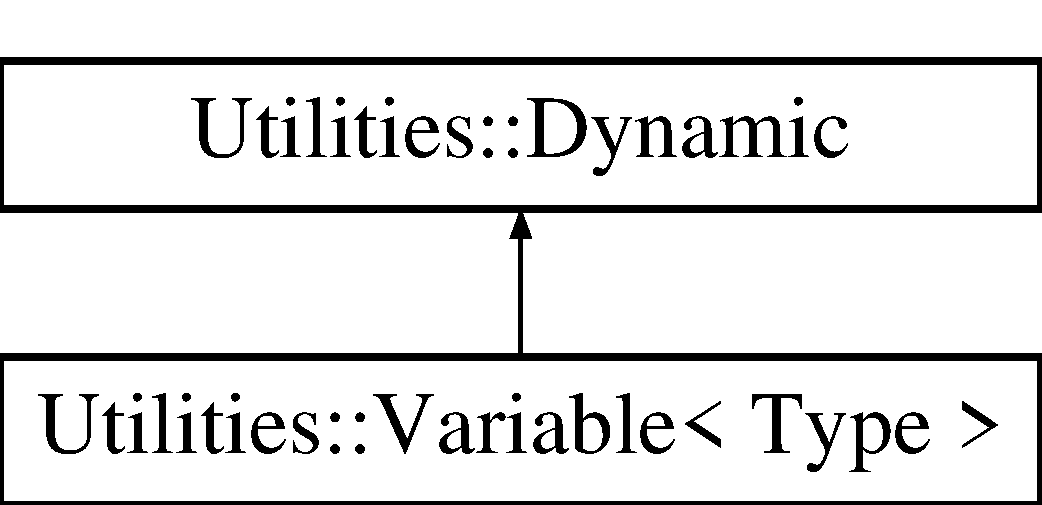
\includegraphics[height=2.000000cm]{classUtilities_1_1Variable}
\end{center}
\end{figure}
\subsection*{Public Member Functions}
\begin{DoxyCompactItemize}
\item 
\hyperlink{classUtilities_1_1Variable_af6f55d5d5c2472b25212828c66b730bc}{Variable} (Type new\+\_\+value)
\item 
virtual \hyperlink{classUtilities_1_1Variable_a4d2bce0bd082e8464b9f193d1e908e0a}{$\sim$\+Variable} ()
\item 
Type \hyperlink{classUtilities_1_1Variable_a2531a59e087062fab302cf487b6bdfa2}{get\+Value} ()
\item 
Type \& \hyperlink{classUtilities_1_1Variable_aec9b6becdc76afca1635280ab81ac41d}{get\+Reference} ()
\item 
void \hyperlink{classUtilities_1_1Variable_af218f1c4f50cbb2f69cc66e8150e05b3}{set\+Value} (Type new\+\_\+value)
\end{DoxyCompactItemize}
\subsection*{Protected Attributes}
\begin{DoxyCompactItemize}
\item 
Type \hyperlink{classUtilities_1_1Variable_ab91417296eea0614f336941a2ecc2944}{value}
\end{DoxyCompactItemize}


\subsection{Constructor \& Destructor Documentation}
\index{Utilities\+::\+Variable@{Utilities\+::\+Variable}!Variable@{Variable}}
\index{Variable@{Variable}!Utilities\+::\+Variable@{Utilities\+::\+Variable}}
\subsubsection[{\texorpdfstring{Variable(\+Type new\+\_\+value)}{Variable(Type new_value)}}]{\setlength{\rightskip}{0pt plus 5cm}template$<$typename Type$>$ {\bf Utilities\+::\+Variable}$<$ Type $>$\+::{\bf Variable} (
\begin{DoxyParamCaption}
\item[{Type}]{new\+\_\+value}
\end{DoxyParamCaption}
)}\hypertarget{classUtilities_1_1Variable_af6f55d5d5c2472b25212828c66b730bc}{}\label{classUtilities_1_1Variable_af6f55d5d5c2472b25212828c66b730bc}
\hyperlink{classUtilities_1_1Variable}{Variable} object constructor 
\begin{DoxyTemplParams}{Template Parameters}
{\em Type} & type of variable \\
\hline
\end{DoxyTemplParams}

\begin{DoxyParams}{Parameters}
{\em new\+\_\+value} & value of new variable \\
\hline
\end{DoxyParams}
\begin{DoxyReturn}{Returns}
none 
\end{DoxyReturn}
\index{Utilities\+::\+Variable@{Utilities\+::\+Variable}!````~Variable@{$\sim$\+Variable}}
\index{````~Variable@{$\sim$\+Variable}!Utilities\+::\+Variable@{Utilities\+::\+Variable}}
\subsubsection[{\texorpdfstring{$\sim$\+Variable()}{~Variable()}}]{\setlength{\rightskip}{0pt plus 5cm}template$<$typename Type$>$ virtual {\bf Utilities\+::\+Variable}$<$ Type $>$\+::$\sim${\bf Variable} (
\begin{DoxyParamCaption}
{}
\end{DoxyParamCaption}
)\hspace{0.3cm}{\ttfamily [virtual]}}\hypertarget{classUtilities_1_1Variable_a4d2bce0bd082e8464b9f193d1e908e0a}{}\label{classUtilities_1_1Variable_a4d2bce0bd082e8464b9f193d1e908e0a}
\hyperlink{classUtilities_1_1Variable}{Variable} object destructor 
\begin{DoxyTemplParams}{Template Parameters}
{\em Type} & type of variable \\
\hline
\end{DoxyTemplParams}
\begin{DoxyReturn}{Returns}
none 
\end{DoxyReturn}


\subsection{Member Function Documentation}
\index{Utilities\+::\+Variable@{Utilities\+::\+Variable}!get\+Reference@{get\+Reference}}
\index{get\+Reference@{get\+Reference}!Utilities\+::\+Variable@{Utilities\+::\+Variable}}
\subsubsection[{\texorpdfstring{get\+Reference()}{getReference()}}]{\setlength{\rightskip}{0pt plus 5cm}template$<$typename Type$>$ Type\& {\bf Utilities\+::\+Variable}$<$ Type $>$\+::get\+Reference (
\begin{DoxyParamCaption}
{}
\end{DoxyParamCaption}
)}\hypertarget{classUtilities_1_1Variable_aec9b6becdc76afca1635280ab81ac41d}{}\label{classUtilities_1_1Variable_aec9b6becdc76afca1635280ab81ac41d}
Get current value by reference 
\begin{DoxyTemplParams}{Template Parameters}
{\em Type} & type of variable \\
\hline
\end{DoxyTemplParams}
\begin{DoxyReturn}{Returns}
value of current leaf 
\end{DoxyReturn}
\index{Utilities\+::\+Variable@{Utilities\+::\+Variable}!get\+Value@{get\+Value}}
\index{get\+Value@{get\+Value}!Utilities\+::\+Variable@{Utilities\+::\+Variable}}
\subsubsection[{\texorpdfstring{get\+Value()}{getValue()}}]{\setlength{\rightskip}{0pt plus 5cm}template$<$typename Type$>$ Type {\bf Utilities\+::\+Variable}$<$ Type $>$\+::get\+Value (
\begin{DoxyParamCaption}
{}
\end{DoxyParamCaption}
)}\hypertarget{classUtilities_1_1Variable_a2531a59e087062fab302cf487b6bdfa2}{}\label{classUtilities_1_1Variable_a2531a59e087062fab302cf487b6bdfa2}
Get current value 
\begin{DoxyTemplParams}{Template Parameters}
{\em Type} & type of variable \\
\hline
\end{DoxyTemplParams}
\begin{DoxyReturn}{Returns}
value of current leaf 
\end{DoxyReturn}
\index{Utilities\+::\+Variable@{Utilities\+::\+Variable}!set\+Value@{set\+Value}}
\index{set\+Value@{set\+Value}!Utilities\+::\+Variable@{Utilities\+::\+Variable}}
\subsubsection[{\texorpdfstring{set\+Value(\+Type new\+\_\+value)}{setValue(Type new_value)}}]{\setlength{\rightskip}{0pt plus 5cm}template$<$typename Type$>$ void {\bf Utilities\+::\+Variable}$<$ Type $>$\+::set\+Value (
\begin{DoxyParamCaption}
\item[{Type}]{new\+\_\+value}
\end{DoxyParamCaption}
)}\hypertarget{classUtilities_1_1Variable_af218f1c4f50cbb2f69cc66e8150e05b3}{}\label{classUtilities_1_1Variable_af218f1c4f50cbb2f69cc66e8150e05b3}
Set value of variable 
\begin{DoxyTemplParams}{Template Parameters}
{\em Type} & type of variable \\
\hline
\end{DoxyTemplParams}

\begin{DoxyParams}{Parameters}
{\em new\+\_\+value} & new value \\
\hline
\end{DoxyParams}
\begin{DoxyReturn}{Returns}
none 
\end{DoxyReturn}


\subsection{Member Data Documentation}
\index{Utilities\+::\+Variable@{Utilities\+::\+Variable}!value@{value}}
\index{value@{value}!Utilities\+::\+Variable@{Utilities\+::\+Variable}}
\subsubsection[{\texorpdfstring{value}{value}}]{\setlength{\rightskip}{0pt plus 5cm}template$<$typename Type$>$ Type {\bf Utilities\+::\+Variable}$<$ Type $>$\+::value\hspace{0.3cm}{\ttfamily [protected]}}\hypertarget{classUtilities_1_1Variable_ab91417296eea0614f336941a2ecc2944}{}\label{classUtilities_1_1Variable_ab91417296eea0614f336941a2ecc2944}
\char`\"{}\+Dynamic\char`\"{} variable 

The documentation for this class was generated from the following file\+:\begin{DoxyCompactItemize}
\item 
utilities.\+h\end{DoxyCompactItemize}

\hypertarget{classUtilities_1_1Variables}{}\doxysection{Utilities\+::Variables Class Reference}
\label{classUtilities_1_1Variables}\index{Utilities::Variables@{Utilities::Variables}}


{\ttfamily \#include $<$utilities.\+h$>$}

\doxysubsection*{Public Member Functions}
\begin{DoxyCompactItemize}
\item 
\mbox{\hyperlink{classUtilities_1_1Variables_a60ebf236218fbefc48cb35e6dcabb2d6}{Variables}} ()
\item 
virtual \mbox{\hyperlink{classUtilities_1_1Variables_a4a67d0d360d70d7a928be6fe48c6753b}{$\sim$\+Variables}} ()
\item 
{\footnotesize template$<$typename Type $>$ }\\void \mbox{\hyperlink{classUtilities_1_1Variables_a7763fc000f45ef3956d61fdf2f783130}{new\+Var}} (std\+::string new\+\_\+name)
\item 
{\footnotesize template$<$typename Type $>$ }\\void \mbox{\hyperlink{classUtilities_1_1Variables_a67029a527f5810a298fc6538b6a634d2}{new\+Var}} (std\+::string new\+\_\+name, Type new\+\_\+value)
\item 
{\footnotesize template$<$typename Type $>$ }\\Type \mbox{\hyperlink{classUtilities_1_1Variables_adff493c2ea6249294a35204fd6b3f852}{get\+Var}} (std\+::string name)
\item 
{\footnotesize template$<$typename Type $>$ }\\Type \& \mbox{\hyperlink{classUtilities_1_1Variables_a58011fc344bd7d5eeb70eaa794f8bb78}{get\+Ref}} (std\+::string name)
\item 
{\footnotesize template$<$typename Type $>$ }\\Type \mbox{\hyperlink{classUtilities_1_1Variables_ad5f59cff15b008435763a81bdac8bcf3}{set\+Var}} (std\+::string name, Type new\+\_\+value)
\end{DoxyCompactItemize}
\doxysubsection*{Protected Member Functions}
\begin{DoxyCompactItemize}
\item 
{\footnotesize template$<$typename Type $>$ }\\\mbox{\hyperlink{classUtilities_1_1Variable}{Variable}}$<$ Type $>$ $\ast$ \mbox{\hyperlink{classUtilities_1_1Variables_a609f89b273fec84499bf782a6109e8f2}{get\+Variable}} (std\+::string name)
\end{DoxyCompactItemize}
\doxysubsection*{Protected Attributes}
\begin{DoxyCompactItemize}
\item 
std\+::map$<$ std\+::string, \mbox{\hyperlink{classUtilities_1_1Dynamic}{Dynamic}} $\ast$ $>$ \mbox{\hyperlink{classUtilities_1_1Variables_acd0a2a9ec3135923b460cdf4e571d478}{variables}}
\end{DoxyCompactItemize}


\doxysubsection{Detailed Description}
A group of \char`\"{}dynamic\char`\"{} variables 

\doxysubsection{Constructor \& Destructor Documentation}
\mbox{\Hypertarget{classUtilities_1_1Variables_a60ebf236218fbefc48cb35e6dcabb2d6}\label{classUtilities_1_1Variables_a60ebf236218fbefc48cb35e6dcabb2d6}} 
\index{Utilities::Variables@{Utilities::Variables}!Variables@{Variables}}
\index{Variables@{Variables}!Utilities::Variables@{Utilities::Variables}}
\doxysubsubsection{\texorpdfstring{Variables()}{Variables()}}
{\footnotesize\ttfamily Utilities\+::\+Variables\+::\+Variables (\begin{DoxyParamCaption}{ }\end{DoxyParamCaption})}

\mbox{\hyperlink{classUtilities_1_1Variables}{Variables}} object constructor \begin{DoxyReturn}{Returns}
none 
\end{DoxyReturn}
\mbox{\Hypertarget{classUtilities_1_1Variables_a4a67d0d360d70d7a928be6fe48c6753b}\label{classUtilities_1_1Variables_a4a67d0d360d70d7a928be6fe48c6753b}} 
\index{Utilities::Variables@{Utilities::Variables}!````~Variables@{$\sim$Variables}}
\index{````~Variables@{$\sim$Variables}!Utilities::Variables@{Utilities::Variables}}
\doxysubsubsection{\texorpdfstring{$\sim$Variables()}{~Variables()}}
{\footnotesize\ttfamily virtual Utilities\+::\+Variables\+::$\sim$\+Variables (\begin{DoxyParamCaption}{ }\end{DoxyParamCaption})\hspace{0.3cm}{\ttfamily [virtual]}}

\mbox{\hyperlink{classUtilities_1_1Variables}{Variables}} object destructor \begin{DoxyReturn}{Returns}
none 
\end{DoxyReturn}


\doxysubsection{Member Function Documentation}
\mbox{\Hypertarget{classUtilities_1_1Variables_a58011fc344bd7d5eeb70eaa794f8bb78}\label{classUtilities_1_1Variables_a58011fc344bd7d5eeb70eaa794f8bb78}} 
\index{Utilities::Variables@{Utilities::Variables}!getRef@{getRef}}
\index{getRef@{getRef}!Utilities::Variables@{Utilities::Variables}}
\doxysubsubsection{\texorpdfstring{getRef()}{getRef()}}
{\footnotesize\ttfamily template$<$typename Type $>$ \\
Type \& Utilities\+::\+Variables\+::get\+Ref (\begin{DoxyParamCaption}\item[{std\+::string}]{name }\end{DoxyParamCaption})}

Get variable in map by reference if it exists 
\begin{DoxyTemplParams}{Template Parameters}
{\em Type} & type of variable \\
\hline
\end{DoxyTemplParams}

\begin{DoxyParams}{Parameters}
{\em name} & name of variable \\
\hline
\end{DoxyParams}
\begin{DoxyReturn}{Returns}
none 
\end{DoxyReturn}
\mbox{\Hypertarget{classUtilities_1_1Variables_adff493c2ea6249294a35204fd6b3f852}\label{classUtilities_1_1Variables_adff493c2ea6249294a35204fd6b3f852}} 
\index{Utilities::Variables@{Utilities::Variables}!getVar@{getVar}}
\index{getVar@{getVar}!Utilities::Variables@{Utilities::Variables}}
\doxysubsubsection{\texorpdfstring{getVar()}{getVar()}}
{\footnotesize\ttfamily template$<$typename Type $>$ \\
Type Utilities\+::\+Variables\+::get\+Var (\begin{DoxyParamCaption}\item[{std\+::string}]{name }\end{DoxyParamCaption})}

Get value of a variable in map if it exists 
\begin{DoxyTemplParams}{Template Parameters}
{\em Type} & type of variable \\
\hline
\end{DoxyTemplParams}

\begin{DoxyParams}{Parameters}
{\em name} & name of variable \\
\hline
\end{DoxyParams}
\begin{DoxyReturn}{Returns}
none 
\end{DoxyReturn}
\mbox{\Hypertarget{classUtilities_1_1Variables_a609f89b273fec84499bf782a6109e8f2}\label{classUtilities_1_1Variables_a609f89b273fec84499bf782a6109e8f2}} 
\index{Utilities::Variables@{Utilities::Variables}!getVariable@{getVariable}}
\index{getVariable@{getVariable}!Utilities::Variables@{Utilities::Variables}}
\doxysubsubsection{\texorpdfstring{getVariable()}{getVariable()}}
{\footnotesize\ttfamily template$<$typename Type $>$ \\
\mbox{\hyperlink{classUtilities_1_1Variable}{Variable}}$<$ Type $>$ $\ast$ Utilities\+::\+Variables\+::get\+Variable (\begin{DoxyParamCaption}\item[{std\+::string}]{name }\end{DoxyParamCaption})\hspace{0.3cm}{\ttfamily [protected]}}

(PROTECTED) Retrieve variable object from map if it exists 
\begin{DoxyTemplParams}{Template Parameters}
{\em Type} & type of variable \\
\hline
\end{DoxyTemplParams}

\begin{DoxyParams}{Parameters}
{\em name} & name of variable \\
\hline
\end{DoxyParams}
\begin{DoxyReturn}{Returns}
none 
\end{DoxyReturn}
\mbox{\Hypertarget{classUtilities_1_1Variables_a7763fc000f45ef3956d61fdf2f783130}\label{classUtilities_1_1Variables_a7763fc000f45ef3956d61fdf2f783130}} 
\index{Utilities::Variables@{Utilities::Variables}!newVar@{newVar}}
\index{newVar@{newVar}!Utilities::Variables@{Utilities::Variables}}
\doxysubsubsection{\texorpdfstring{newVar()}{newVar()}\hspace{0.1cm}{\footnotesize\ttfamily [1/2]}}
{\footnotesize\ttfamily template$<$typename Type $>$ \\
void Utilities\+::\+Variables\+::new\+Var (\begin{DoxyParamCaption}\item[{std\+::string}]{new\+\_\+name }\end{DoxyParamCaption})}

Add blank variable to map 
\begin{DoxyTemplParams}{Template Parameters}
{\em Type} & type of new variable \\
\hline
\end{DoxyTemplParams}

\begin{DoxyParams}{Parameters}
{\em new\+\_\+name} & name of new variable \\
\hline
\end{DoxyParams}
\begin{DoxyReturn}{Returns}
none 
\end{DoxyReturn}
\mbox{\Hypertarget{classUtilities_1_1Variables_a67029a527f5810a298fc6538b6a634d2}\label{classUtilities_1_1Variables_a67029a527f5810a298fc6538b6a634d2}} 
\index{Utilities::Variables@{Utilities::Variables}!newVar@{newVar}}
\index{newVar@{newVar}!Utilities::Variables@{Utilities::Variables}}
\doxysubsubsection{\texorpdfstring{newVar()}{newVar()}\hspace{0.1cm}{\footnotesize\ttfamily [2/2]}}
{\footnotesize\ttfamily template$<$typename Type $>$ \\
void Utilities\+::\+Variables\+::new\+Var (\begin{DoxyParamCaption}\item[{std\+::string}]{new\+\_\+name,  }\item[{Type}]{new\+\_\+value }\end{DoxyParamCaption})}

Add new variable to map 
\begin{DoxyTemplParams}{Template Parameters}
{\em Type} & type of new variable \\
\hline
\end{DoxyTemplParams}

\begin{DoxyParams}{Parameters}
{\em new\+\_\+name} & name of new variable \\
\hline
{\em new\+\_\+value} & value of new variable \\
\hline
\end{DoxyParams}
\begin{DoxyReturn}{Returns}
none 
\end{DoxyReturn}
\mbox{\Hypertarget{classUtilities_1_1Variables_ad5f59cff15b008435763a81bdac8bcf3}\label{classUtilities_1_1Variables_ad5f59cff15b008435763a81bdac8bcf3}} 
\index{Utilities::Variables@{Utilities::Variables}!setVar@{setVar}}
\index{setVar@{setVar}!Utilities::Variables@{Utilities::Variables}}
\doxysubsubsection{\texorpdfstring{setVar()}{setVar()}}
{\footnotesize\ttfamily template$<$typename Type $>$ \\
Type Utilities\+::\+Variables\+::set\+Var (\begin{DoxyParamCaption}\item[{std\+::string}]{name,  }\item[{Type}]{new\+\_\+value }\end{DoxyParamCaption})}

Set value of a variable in map if it exists 
\begin{DoxyTemplParams}{Template Parameters}
{\em Type} & type of variable \\
\hline
\end{DoxyTemplParams}

\begin{DoxyParams}{Parameters}
{\em name} & name of variable \\
\hline
{\em new\+\_\+value} & new value for variable \\
\hline
\end{DoxyParams}
\begin{DoxyReturn}{Returns}
none 
\end{DoxyReturn}


\doxysubsection{Member Data Documentation}
\mbox{\Hypertarget{classUtilities_1_1Variables_acd0a2a9ec3135923b460cdf4e571d478}\label{classUtilities_1_1Variables_acd0a2a9ec3135923b460cdf4e571d478}} 
\index{Utilities::Variables@{Utilities::Variables}!variables@{variables}}
\index{variables@{variables}!Utilities::Variables@{Utilities::Variables}}
\doxysubsubsection{\texorpdfstring{variables}{variables}}
{\footnotesize\ttfamily std\+::map$<$std\+::string, \mbox{\hyperlink{classUtilities_1_1Dynamic}{Dynamic}}$\ast$$>$ Utilities\+::\+Variables\+::variables\hspace{0.3cm}{\ttfamily [protected]}}

Map of dynamic variables 

The documentation for this class was generated from the following file\+:\begin{DoxyCompactItemize}
\item 
/\+Users/jguiang/\+Projects/rapido/utilities.\+h\end{DoxyCompactItemize}

%--- End generated contents ---

% Index
\backmatter
\newpage
\phantomsection
\clearemptydoublepage
\addcontentsline{toc}{chapter}{Index}
\printindex

\end{document}
